\documentclass[cn,11pt,chinese]{elegantbook}
\usepackage{minted}

\title{尚硅谷Flink教程}
\subtitle{理论与实践}

\author{左元}
\institute{尚硅谷大数据组}
\date{April 12, 2020}
\version{3.11}
\bioinfo{自定义}{信息}

\extrainfo{温柔正确的人总是难以生存，因为这世界既不温柔，也不正确。—— 比企谷八幡}

\logo{logo-blue.png}
\cover{cover.jpg}

% 本文档命令
\usepackage{array}
\newcommand{\ccr}[1]{\makecell{{\color{#1}\rule{1cm}{1cm}}}}

\begin{document}

\maketitle
\frontmatter

\chapter*{特别声明}
\markboth{Introduction}{前言}

在过去的 2019 年，\href{https://elegantlatex.org/}{Elegant\LaTeX{}} 系列模板均逐步上线 \href{https://github.com/ElegantLaTeX}{GitHub}、\href{https://ctan.org/pkg/elegantbook}{CTAN}、\href{https://www.overleaf.com/latex/templates/elegantbook-template/zpsrbmdsxrgy}{Overleaf} 以及 \href{https://gitee.com/ElegantLaTeX/ElegantBook}{Gitee} 上。截止到 2019 年底，ElegantNote、ElegantBook、ElegantPaper 三个模板在 GitHub 上的收藏数达到了 194、333 和 220，从 2019 年 5 月开启捐赠之后收到了用户 33 笔合计超过 1500 元的捐赠，用户群人数也超过了 400 人。这些数字的背后，反映出 Elegant\LaTeX{} 越来越受用户的喜爱，在此非常感谢大家。

但是，我想声明的是：

\begin{center}
  由于某些原因，Elegant\LaTeX{} 项目 \underline{不再接受}\textbf{任何}非我本人预约的提交。
\end{center}

我是一个理想主义者，关于这个模板，我有自己的想法。我所关心的是，我周围的人能方便使用 \LaTeX{} 以及此模板，我自己会为自己的东西感到开心。如果维护模板让我不开心，那我就不会再维护了。诚然这个模板并不是完美的，但是相比 2.x 好很多了，这些改进离不开大家的反馈、China\TeX{} 和逐鹿人的鼓励以及支援人员的帮助！

\underline{如果你无法认同我的想法，建议直接删除本模板。}

\vskip 1.5cm

\begin{flushright}
Ethan Deng\\
February 10, 2020
\end{flushright}

\tableofcontents
%\listofchanges

\mainmatter

\chapter{有状态的流式处理}

Apache Flink是一个分布式流处理器，具有直观和富有表现力的API，可实现有状态的流处理应用程序。它以容错的方式有效地大规模运行这些应用程序。 Flink于2014年4月加入Apache软件基金会作为孵化项目，并于2015年1月成为顶级项目。从一开始，Flink就拥有一个非常活跃且不断增长的用户和贡献者社区。到目前为止，已有超过五百人为Flink做出贡献，并且它已经发展成为最复杂的开源流处理引擎之一，并得到了广泛采用的证明。 Flink为不同行业和全球的许多公司和企业提供大规模的商业关键应用。

流处理技术在大大小小的公司中越来越受欢迎，因为它为许多已建立的用例（如数据分析，ETL和事务应用程序）提供了卓越的解决方案，同时也促进了新颖的应用程序，软件架构和商机。接下来我们将讨论，为什么有状态流处理变得如此受欢迎并评估其潜力。我们首先回顾传统的数据应用程序架构并指出它们的局限性。接下来，我们介绍基于状态流处理的应用程序设计 与传统方法相比，它具有许多有趣的特征最后，我们简要讨论开源流处理器的发展，并在本地Flink实例上运行流应用程序。

\section{传统数据处理架构}

数十年来，数据和数据处理在企业中无处不在。多年来，数据的收集和使用一直在增长，公司已经设计并构建了基础架构来管理数据。大多数企业实施的传统架构区分了两种类型的数据处理：事务处理（OLTP）和分析处理（OLAP）。

\subsection{事务处理}

公司将各种应用程序用于日常业务活动，例如企业资源规划（ERP）系统，客户关系管理（CRM）软件和基于Web的应用程序。这些系统通常设计有单独的层，用于数据处理（应用程序本身）和数据存储（事务数据库系统），如图所示。

\begin{figure}[htbp]
  \centering
  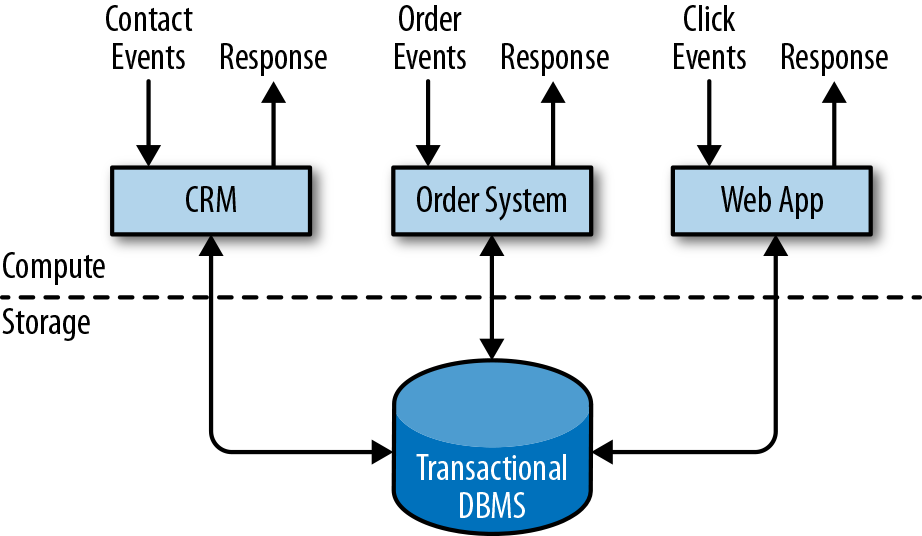
\includegraphics[width=0.7\textwidth]{images/spaf_0101.png}
  \caption{事务处理}
\end{figure}

应用程序通常连接到外部服务或直接面向用户，并持续处理传入的事件，如网站上的订单，电子邮件或点击。处理事件时，应用程序将会读取远程数据库的状态，或者通过运行事务来更新它。通常，一个数据库系统可以服务于多个应用程序，它们有时会访问相同的数据库或表。

当应用程序需要扩展时，这样的设计可能会导致问题。由于多个应用程序可能会同时用到相同的数据表示，或者共享相同的基础设施，因此想要更改表的结构或扩展数据库，就需要仔细的规划和大量的工作。克服紧耦合应用程序的最新方法是微服务设计模式。微服务被设计为小型、完备且独立的应用程序。他们遵循UNIX的理念，即“只做一件事并且把它做好”。通过将几个微服务相互连接来构建更复杂的应用程序，这些微服务仅通过标准化接口（例如RESTful HTTP连接）进行通信。由于微服务严格地彼此分离并且仅通过明确定义的接口进行通信，因此每个微服务都可以用不同技术栈来实现，包括编程语言、类库和数据存储。微服务和所有必需的软件和服务通常捆绑在一起并部署在独立的容器中。下图描绘了一种微服务架构。

\begin{figure}[htbp]
  \centering
  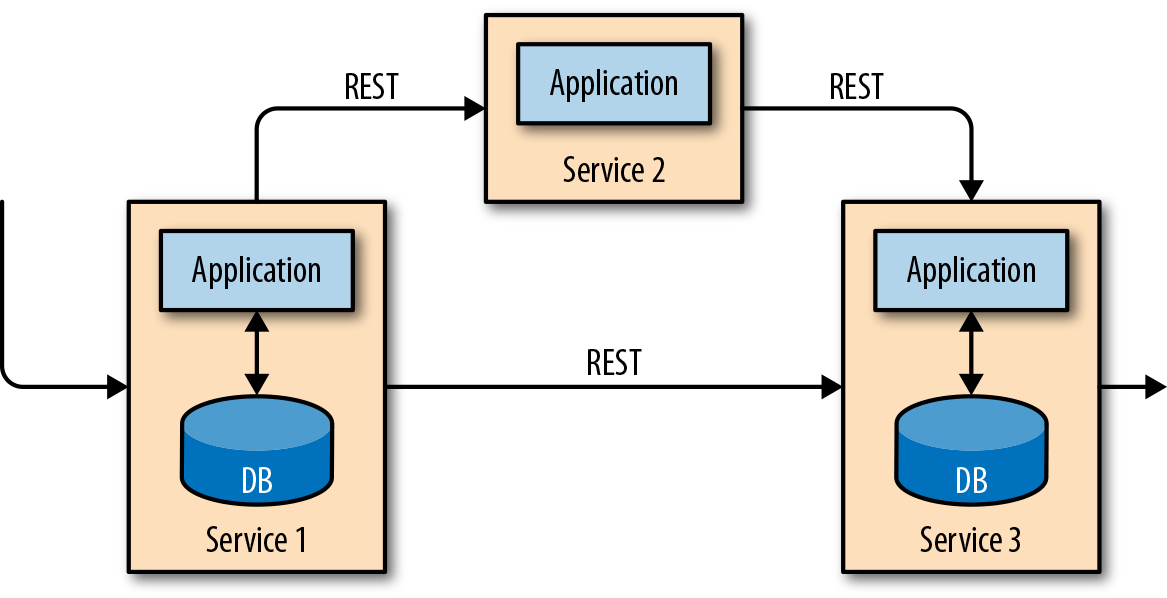
\includegraphics[width=0.7\textwidth]{images/spaf_0102.png}
  \caption{事务处理}
\end{figure}

\subsection{分析处理}

大量数据存储在公司的各种事务数据库系统中，它们可以为公司业务运营提供宝贵的参考意见。例如，分析订单处理系统的数据，可以获得销量随时间的增长曲线；可以识别延迟发货的原因；还可以预测未来的销量以便提前调整库存。但是，事务数据通常分布在多个数据库中，它们往往汇总起来联合分析时更有价值。而且，数据通常需要转换为通用格式。

所以我们一般不会直接在事务数据库上运行分析查询，而是复制数据到数据仓库。数据仓库是对工作负载进行分析和查询的专用数据存储。为了填充数据仓库，需要将事务数据库系统管理的数据复制过来。将数据复制到数据仓库的过程称为extract-transform-load（ETL）。 ETL过程从事务数据库中提取数据，将其转换为某种通用的结构表示，可能包括验证，值的规范化，编码，重复数据删除（去重）和模式转换，最后将其加载到分析数据库中。 ETL过程可能非常复杂，并且通常需要技术复杂的解决方案来满足性能要求。 ETL过程需要定期运行以保持数据仓库中的数据同步。

将数据导入数据仓库后，可以查询和分析数据。通常，在数据仓库上执行两类查询。第一种类型是定期报告查询，用于计算与业务相关的统计信息，比如收入、用户增长或者输出的产量。这些指标汇总到报告中，帮助管理层评估业务的整体健康状况。第二种类型是即席查询，旨在提供特定问题的答案并支持关键业务决策，例如收集统计在投放商业广告上的花费，和获取的相应收入，以评估营销活动的有效性。两种查询由批处理方式由数据仓库执行，如图所示。

\begin{figure}[htbp]
  \centering
  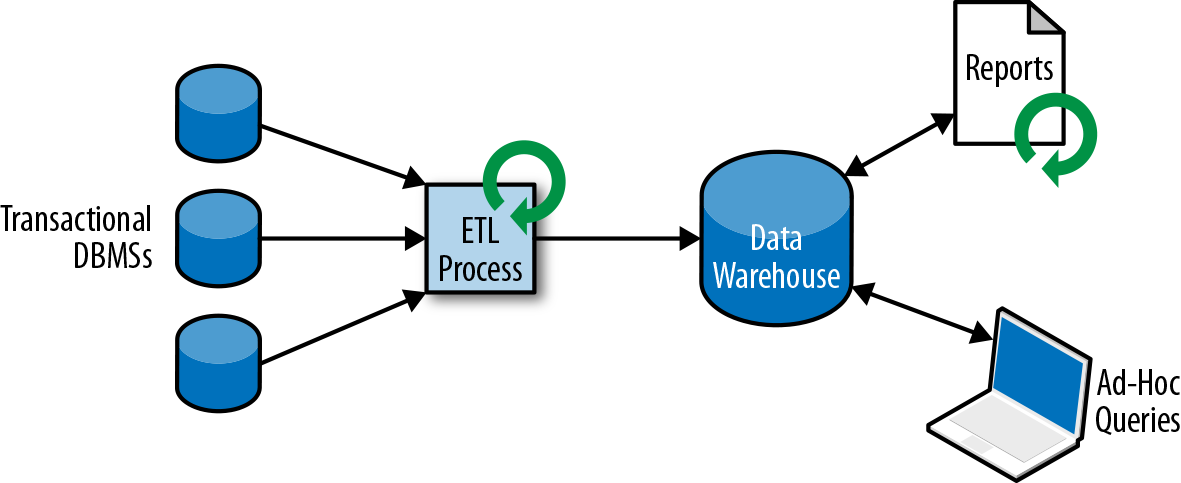
\includegraphics[width=0.7\textwidth]{images/spaf_0103.png}
  \caption{事务处理}
\end{figure}

如今，Apache Hadoop生态系统的组件，已经是许多企业IT基础架构中不可或缺的组成部分。现在的做法不是直接将所有数据都插入关系数据库系统，而是将大量数据（如日志文件，社交媒体或Web点击日志）写入Hadoop的分布式文件系统（HDFS）、S3或其他批量数据存储库，如Apache HBase，以较低的成本提供大容量存储容量。驻留在此类存储系统中的数据可以通过SQL-on-Hadoop引擎查询和处理，例如Apache Hive，Apache Drill或Apache Impala。但是，基础结构与传统数据仓库架构基本相同。

\section{有状态的流式处理}

日常生活中，所有数据都是作为连续的事件流创建的。比如网站或者移动应用中的用户交互动作，订单的提交，服务器日志或传感器测量数据：所有这些都是事件流。实际上，很少有应用场景，能一次性地生成所需要的完整（有限）数据集。实际应用中更多的是无限事件流。有状态的流处理就是用于处理这种无限事件流的应用程序设计模式，在公司的IT基础设施中有广泛的应用场景。在我们讨论其用例之前，我们将简要介绍有状态流处理的工作原理。

如果我们想要无限处理事件流，并且不愿意繁琐地每收到一个事件就记录一次，那这样的应用程序就需要是有状态的，也就是说能够存储和访问中间数据。当应用程序收到一个新事件时，它可以从状态中读取数据，或者向该状态写入数据，总之可以执行任何计算。原则上讲，我们可以在各种不同的地方存储和访问状态，包括程序变量（内存）、本地文件，还有嵌入式或外部数据库。

Apache Flink将应用程序状态，存储在内存或者嵌入式数据库中。由于Flink是一个分布式系统，因此需要保护本地状态以防止在应用程序或计算机故障时数据丢失。 Flink通过定期将应用程序状态的一致性检查点（check point）写入远程且持久的存储，来保证这一点。状态、状态一致性和Flink的检查点将在后面的章节中更详细地讨论，但是，现在，下图显示了有状态的流式Flink应用程序。

\begin{figure}[htbp]
  \centering
  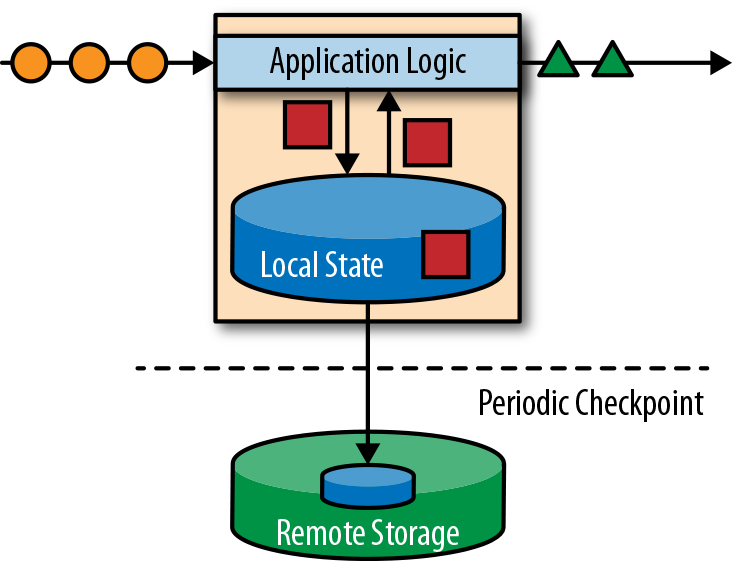
\includegraphics[width=0.7\textwidth]{images/spaf_0104.png}
  \caption{有状态的流式处理}
\end{figure}

有状态的流处理应用程序，通常从事件日志中提取输入事件。事件日志就用来存储和分发事件流。事件被写入持久的仅添加（append-only）日志，这意味着无法更改写入事件的顺序。写入事件日志的流，可以被相同或不同的消费者多次读取。由于日志的仅附加（append-only）属性，事件始终以完全相同的顺序发布给所有消费者。现在已有几种事件日志系统，其中Apache Kafka是最受欢迎的，可以作为开源软件使用，或者是云计算提供商提供的集成服务。

在Flink上运行的有状态的流处理应用程序，是很有意思的一件事。在这个架构中，事件日志会按顺序保留输入事件，并且可以按确定的顺序重播它们。如果发生故障，Flink将从先前的检查点（check point）恢复其状态，并重置事件日志上的读取位置，这样就可以恢复整个应用。应用程序将重放（并快进）事件日志中的输入事件，直到它到达流的尾部。此技术一般用于从故障中恢复，但也可用于更新应用程序、修复bug或者修复以前发出的结果，另外还可以用于将应用程序迁移到其他群集，或使用不同的应用程序版本执行A / B测试。

如前所述，有状态的流处理是一种通用且灵活的设计架构，可用于许多不同的场景。在下文中，我们提出了三类通常使用有状态流处理实现的应用程序：（1）事件驱动应用程序，（2）数据管道应用程序，以及（3）数据分析应用程序。

我们将应用程序分类描述，是为了强调有状态流处理适用于多种业务场景；而实际的应用中，往往会具有以上多种情况的特征。

\subsection{事件驱动应用程序}

事件驱动的应用程序是有状态的流应用程序，它们使用特定的业务逻辑来提取事件流并处理事件。根据业务逻辑，事件驱动的应用程序可以触发诸如发送警报、或电子邮件之类的操作，或者将事件写入向外发送的事件流以供另一个应用程序使用。

事件驱动应用程序的典型场景包括：

\begin{itemize}
    \item 实时推荐（例如，在客户浏览零售商网站时推荐产品）
    \item 行为模式检测或复杂事件处理（例如，用于信用卡交易中的欺诈检测）
    \item 异常检测（例如，检测侵入计算机网络的尝试）
\end{itemize}

事件驱动应用程序是微服务的演变。它们通过事件日志而不是REST调用进行通信，并将应用程序数据保存为本地状态，而不是将其写入外部数据存储区（例如关系数据库或键值数据库）。下图显示了由事件驱动的流应用程序组成的服务架构。

\begin{figure}[htbp]
  \centering
  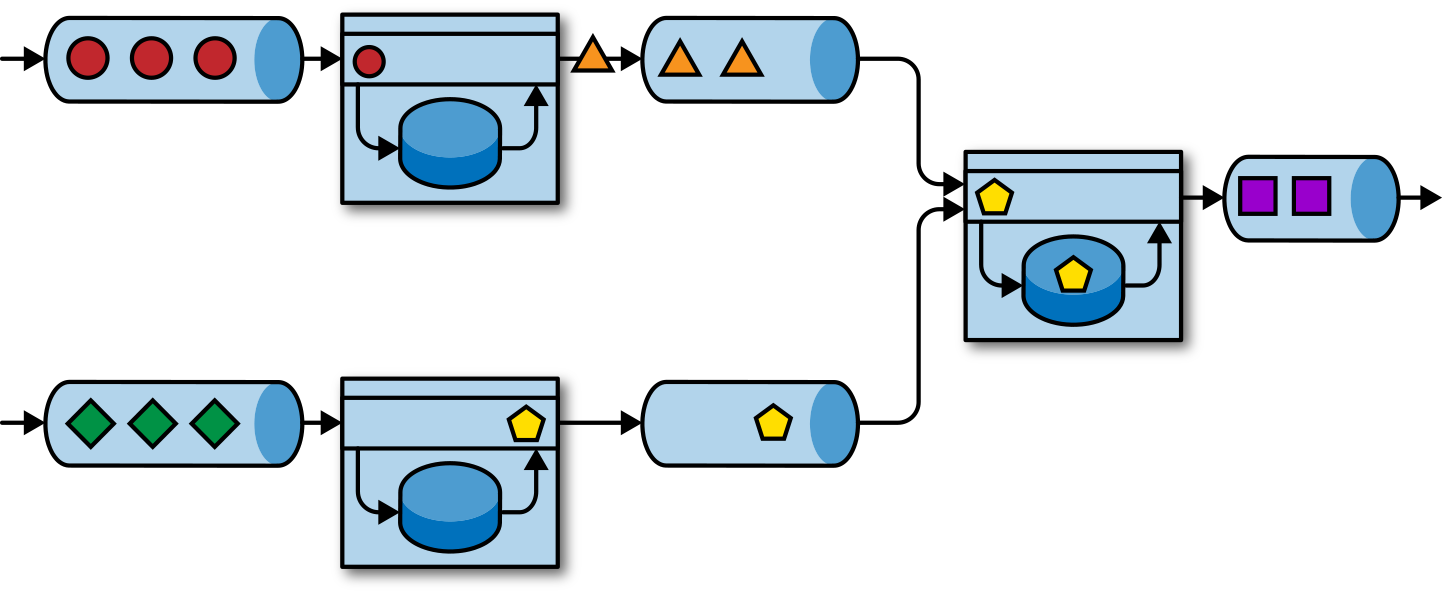
\includegraphics[width=0.7\textwidth]{images/spaf_0105.png}
  \caption{事件驱动}
\end{figure}

上图中的应用程序通过事件日志连接。一个应用程序将其输出发送到事件日志通道（kafka），另一个应用程序使用其他应用程序发出的事件。事件日志通道将发送者和接收者分离，并提供异步、非阻塞的事件传输。每个应用程序都可以是有状态的，并且可以本地管理自己的状态而无需访问外部数据存储。应用程序也可以单独处理和扩展。

与事务性应用程序或微服务相比，事件驱动的应用程序具有多种优势。与读写远程数据库相比，本地状态访问提供了非常好的性能。扩展性和容错性都由流处理器来保证，并且以事件日志作为输入源，应用程序的整个输入数据可以可靠地存储，并且可以确定性地重放。此外，Flink可以将应用程序的状态重置为先前的保存点（save point），从而可以在不丢失状态的情况下更新或重新扩展应用程序。

事件驱动的应用程序对运行它们的流处理器有很高的要求，并不是所有流处理器都适合运行事件驱动的应用程序。 API的表现力，以及对状态处理和事件时间支持的程度，决定了可以实现和执行的业务逻辑。这方面取决于流处理器的API，主要看它能提供什么样的状态类型，以及它对事件时间处理的支持程度。此外，精确一次（exactly-once）的状态一致性和扩展应用程序的能力是事件驱动应用程序的基本要求。 Apache Flink符合所有的这些要求，是运行此类应用程序的一个非常好的选择。

\subsection{数据管道}

当今的IT架构包括许多不同的数据存储，例如关系型数据库和专用数据库系统、事件日志、分布式文件系统，内存中的缓存和搜索索引。所有这些系统都以不同的格式和数据结构存储数据，为其特定的访问模式提供最佳性能。公司通常将相同的数据存储在多个不同的系统中，以提高数据访问的性能。例如，网上商店中提供的产品的信息，可以存储在交易数据库中，同时也存储在缓存（如redis）和搜索索引（如ES）中。由于数据的这种复制，数据存储必须保持同步。

在不同存储系统中同步数据的传统方法是定期ETL作业。但是，它们不能满足当今许多场景的延迟要求。另一种方法是使用事件日志（event log）来发布更新。更新将写入事件日志并由事件日志分发。日志的消费者获取到更新之后，将更新合并到受影响的数据存储中。根据使用情况，传输的数据可能需要标准化、使用外部数据进行扩展，或者在目标数据存储提取之前进行聚合。

以较低的延迟，来提取、转换和插入数据是有状态流处理应用程序的另一个常见应用场景。这种类型的应用程序称为数据管道（data pipeline）。数据管道必须能够在短时间内处理大量数据。操作数据管道的流处理器还应具有许多源（source）和接收器（sink）的连接器，以便从各种存储系统读取数据并将数据写入各种存储系统。当然，同样地，Flink完成了所有这些功能。

\subsection{流分析}

ETL作业定期将数据导入数据存储区，数据的处理是由即席查询（用户自定义查询）或设定好的通常查询来做的。无论架构是基于数据仓库还是基于Hadoop生态系统的组件，这都是批处理。多年来最好的处理方式就是，定期将数据加载到数据分析系统中，但它给分析管道带了的延迟相当大，而且无法避免。

根据设定好的时间间隔，可能需要数小时或数天才能将数据点包含在报告中。我们前面已经提到，数据管道可以实现低延迟的ETL，所以在某种程度上，可以通过使用数据管道将数据导入存储区来减少延迟。但是，即使持续不停地进行ETL操作，在用查询来处理事件之前总会有延迟。虽然这种延迟在过去可能是可以接受的，但是今天的应用程序，往往要求必须能够实时收集数据，并立即对其进行操作（例如，在手机游戏中去适应不断变化的条件，或者在电商网站中提供个性化的用户体验）。

流式分析应用程序不是等待定期触发，而是连续地提取事件流，并且通过纳入最新事件来更新其计算结果，这个过程是低延迟的。这有些类似于数据库中用于更新视图（views）的技术。通常，流应用程序将其结果存储在支持更新的外部数据存储中，例如数据库或键值（key-value）存储。流分析应用程序的实时更新结果可用于驱动监控仪表板（dashboard）应用程序，如下图所示。

\begin{figure}[htbp]
  \centering
  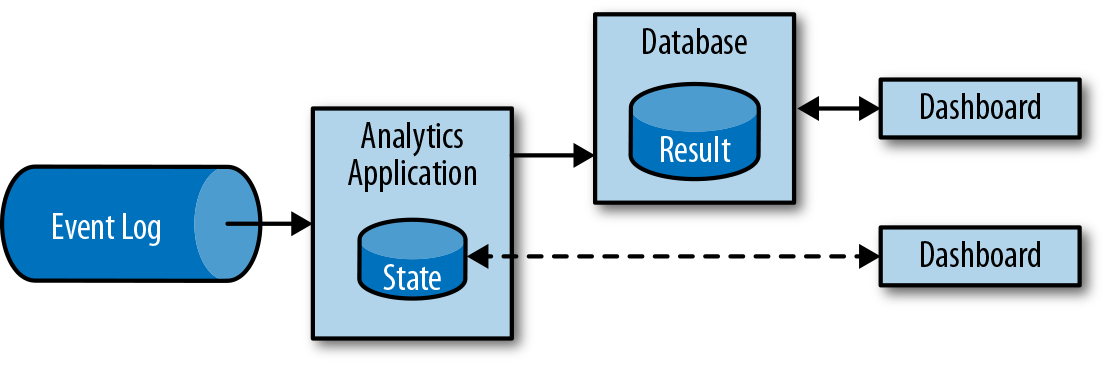
\includegraphics[width=0.7\textwidth]{images/spaf_0106.png}
  \caption{流分析}
\end{figure}

流分析应用程序最大的优势就是，将每个事件纳入到分析结果所需的时间短得多。除此之外，流分析应用程序还有另一个不太明显的优势。传统的分析管道由几个独立的组件组成，例如ETL过程、存储系统、对于基于Hadoop的环境，还包括用于触发任务（jobs）的数据处理和调度程序。相比之下，如果我们运行一个有状态流应用程序，那么流处理器就会负责所有这些处理步骤，包括事件提取、带有状态维护的连续计算以及更新结果。此外，流处理器可以从故障中恢复，并且具有精确一次（exactly-once）的状态一致性保证，还可以调整应用程序的计算资源。像Flink这样的流处理器还支持事件时间（event-time）处理，这可以保证产生正确和确定的结果，并且能够在很短的时间内处理大量数据。

流分析应用程序通常用于：

\begin{itemize}
    \item 监控手机网络的质量分析
    \item 移动应用中的用户行为
    \item 实时数据的即席分析
\end{itemize}

虽然我们不在此处介绍，但Flink还提供对流上的分析SQL查询的支持。

\section{开源流处理的演进}

数据流处理并不是一项新技术。一些最初的研究原型和商业产品可以追溯到20世纪90年代（1990s）。然而，在很大程度上，过去采用的流处理技术是由成熟的开源流处理器驱动的。如今，分布式开源流处理器在不同行业的许多企业中，处理着核心业务应用，比如电商、社交媒体、电信、游戏和银行等。开源软件是这一趋势的主要驱动力，主要原因有两个：

\begin{itemize}
    \item 开源流处理软件是大家每一个人都可以评估和使用的产品。
    \item 由于许多开源社区的努力，可扩展流处理技术正在迅速成熟和发展。
\end{itemize}

仅仅一个Apache软件基金会就支持了十几个与流处理相关的项目。新的分布式流处理项目不断进入开源阶段，并不断增加新的特性和功能。开源社区不断改进其项目的功能，并正在推动流处理的技术边界。我们将简要介绍一下过去，看看开源流处理的起源和今天的状态。

第一代分布式开源流处理器（2011）专注于具有毫秒延迟的事件处理，并提供了在发生故障时防止事件丢失的保证。这些系统具有相当低级的API，并且对于流应用程序的准确性和结果的一致性，不提供内置支持，因为结果会取决于到达事件的时间和顺序。另外，即使事件没有丢失，也可能不止一次地处理它们。与批处理器相比，第一代开源流处理器牺牲了结果准确性，用来获得更低的延迟。为了让当时的数据处理系统，可以同时提供快速和准确的结果，人们设计了所谓的lambda架构，如图所示。

\begin{figure}[htbp]
  \centering
  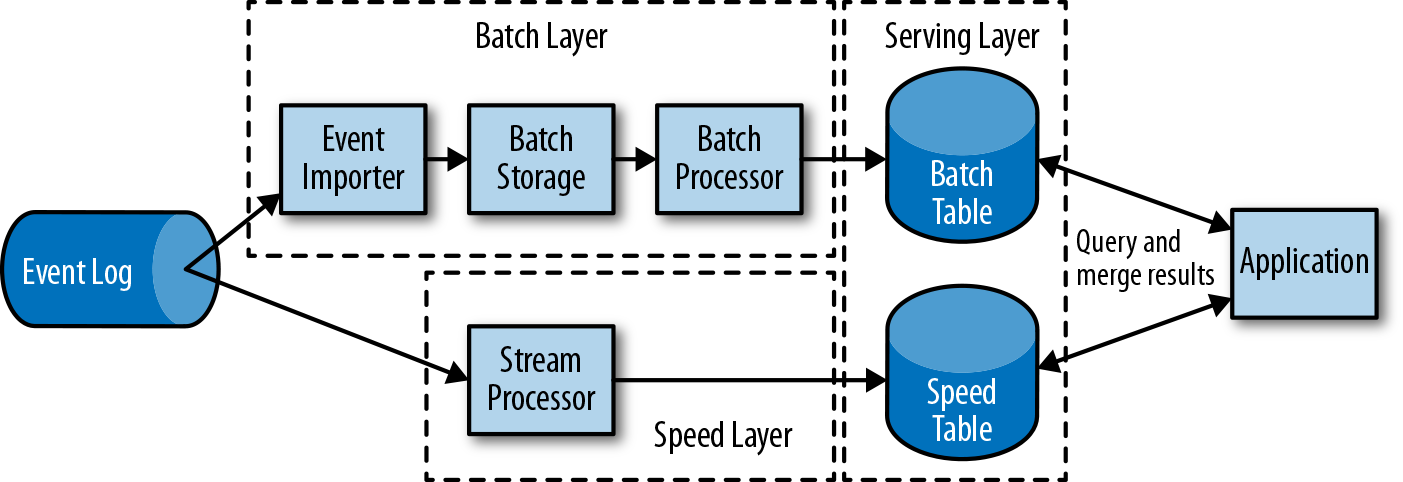
\includegraphics[width=0.7\textwidth]{images/spaf_0107.png}
  \caption{lambda架构}
\end{figure}

lambda架构增强了传统的批处理架构，其“快速层”（speed layer）由低延迟的流处理器来支持。数据到达之后由流处理器提取出来，并写入批处理存储。流处理器近乎实时地计算近似结果并将它们写入“快速表”（speed table）。批处理器定期处理批量存储中的数据，将准确的结果写入批处理表，并从速度表中删除相应的不准确结果。应用程序会合并快速表中的近似结果和批处理表中的准确结果，然后消费最终的结果。

lambda架构现在已经不再是最先进的，但仍在许多地方使用。该体系结构的最初目标是改善原始批处理分析体系结构的高延迟。但是，它有一些明显的缺点。首先，它需要对一个应用程序，做出两个语义上等效的逻辑实现，用于两个独立的、具有不同API的处理系统。其次，流处理器计算的结果只是近似的。第三，lambda架构很难建立和维护。

通过在第一代基础上进行改进，下一代分布式开源流处理器（2013）提供了更好的故障保证，并确保在发生故障时，每个输入记录仅对结果产生一次影响（exactly -once）。此外，编程API从相当低级的操作符接口演变为高级API。但是，一些改进（例如更高的吞吐量和更好的故障保证）是以将处理延迟从毫秒增加到几秒为代价的。此外，结果仍然取决于到达事件的时间和顺序。

第三代分布式开源流处理器（2015）解决了结果对到达事件的时间和顺序的依赖性。结合精确一次（exactly-once）的故障语义，这一代系统是第一个具有计算一致性和准确结果的开源流处理器。通过基于实际数据来计算结果（“重演”数据），这些系统还能够以与“实时”数据相同的方式处理历史数据。另一个改进是解决了延迟/吞吐量无法同时保证的问题。先前的流处理器仅能提供高吞吐量或者低延迟（其中之一），而第三代系统能够同时提供这两个特性。这一代的流处理器使得lambda架构过时了。当然，这一代流处理以flink为代表。

除了目前讨论的特性，例如容错、性能和结果准确性之外，流处理器还不断添加新的操作功能，例如高可用性设置，与资源管理器（如YARN或Kubernetes）的紧密集成，以及能够动态扩展流应用程序。其他功能包括：支持升级应用程序代码，或将作业迁移到其他群集或新版本的流处理器，而不会丢失当前状态。

\section{Flink简介}

Apache Flink是第三代分布式流处理器，它拥有极富竞争力的功能。它提供准确的大规模流处理，具有高吞吐量和低延迟。特别的是，以下功能使Flink脱颖而出：

\begin{itemize}
    \item 事件时间（event-time）和处理时间（processing-tme）语义。即使对于无序事件流，事件时间（event-time）语义仍然能提供一致且准确的结果。而处理时间（processing-time）语义可用于具有极低延迟要求的应用程序。
    \item 精确一次（exactly-once）的状态一致性保证。
    \item 每秒处理数百万个事件，毫秒级延迟。 Flink应用程序可以扩展为在数千个核（cores）上运行。
    \item 分层API，具有不同的权衡表现力和易用性。本书介绍了DataStream API和过程函数（process function），为常见的流处理操作提供原语，如窗口和异步操作，以及精确控制状态和时间的接口。本书不讨论Flink的关系API，SQL和LINQ风格的Table API。
    \item 连接到最常用的存储系统，如Apache Kafka，Apache Cassandra，Elasticsearch，JDBC，Kinesis和（分布式）文件系统，如HDFS和S3。
    \item 由于其高可用的设置（无单点故障），以及与Kubernetes，YARN和Apache Mesos的紧密集成，再加上从故障中快速恢复和动态扩展任务的能力，Flink能够以极少的停机时间7*24全天候运行流应用程序。
    \item 能够更新应用程序代码并将作业（jobs）迁移到不同的Flink集群，而不会丢失应用程序的状态。
    \item 详细且可自定义的系统和应用程序指标集合，以提前识别问题并对其做出反应。
    \item 最后但同样重要的是，Flink也是一个成熟的批处理器。
\end{itemize}

除了这些功能之外，Flink还是一个非常易于开发的框架，因为它易于使用的API。嵌入式执行模式，可以在单个JVM进程中启动应用程序和整个Flink系统，这种模式一般用于在IDE中运行和调试Flink作业。在开发和测试Flink应用程序时，此功能非常有用。

\section{编写第一个Flink程序}

\subsection{在IDEA中编写Flink程序}

\begin{enumerate}
\item 使用Intellij IDEA创建一个Maven新项目
\item 勾选Create from archetype，然后点击Add Archetype按钮
\item GroupId中输入org.apache.flink，ArtifactId中输入flink-quickstart-java，Version中输入Flink的版本号，然后点击OK
\item 点击向右箭头，出现下拉列表，选中flink-quickstart-java:版本号，点击Next
\item Name中输入FlinkTutorial，GroupId中输入com.atguigu，ArtifactId中输入FlinkTutorial，点击Next
\item 最好使用IDEA默认的Maven工具：Bundled（Maven 3），点击Finish，等待一会儿，项目就创建好了
\end{enumerate}

编写\texttt{WordCount.java}程序

\begin{minted}[linenos,breaklines,fontsize=\footnotesize]{java}
public class WordCount {

    public static void main(String[] args) throws Exception {
        final StreamExecutionEnvironment env = StreamExecutionEnvironment.getExecutionEnvironment();
        env.setParallelism(1);

        DataStream<String> stream = env.fromElements("Hello World", "Hello World");

        stream
                .flatMap(new Tokenizer())
                .keyBy(r -> r.f0)
                .sum(1)
                .print();

        env.execute("单词计数");
    }

    public static class Tokenizer implements FlatMapFunction<String, Tuple2<String, Integer>> {
        @Override
        public void flatMap(String value, Collector<Tuple2<String, Integer>> out) throws Exception {
            String[] stringList = value.split("\\s");
            for (String s : stringList) {
                out.collect(Tuple2.of(s, 1));
            }
        }
    }
}
\end{minted}

\subsection{下载Flink运行时环境，提交Jar包的运行方式}

先下载压缩包，然后进行解压。然后进入文件夹。

\begin{minted}[linenos,breaklines,fontsize=\footnotesize]{bash}
$ ./bin/start-cluster.sh
\end{minted}

可以打开Flink WebUI查看集群状态：http://localhost:8081

在IDEA中使用maven package打包。

提交打包好的JAR包：

\begin{minted}[linenos,breaklines,fontsize=\footnotesize]{bash}
$ ./bin/flink run 打包好的JAR包的绝对路径
\end{minted}

停止Flink集群

\begin{minted}[linenos,breaklines,fontsize=\footnotesize]{bash}
$ ./bin/stop-cluster.sh
\end{minted}

查看标准输出日志的位置，在log文件夹中。

\begin{minted}[linenos,breaklines,fontsize=\footnotesize]{bash}
$ cd log/
\end{minted}

\chapter{流处理基础}

\section{数据流编程}

在我们深入研究流处理的基础知识之前，让我们来看看在数据流程编程的背景和使用的术语。

\subsection{数据流图}

顾名思义，数据流程序描述了数据如何在算子之间流动。数据流程序通常表示为有向图，其中节点称为算子，用来表示计算，边表示数据之间的依赖性。算子是数据流程序的基本功能单元。他们从输入消耗数据，对它们执行计算，并生成数据输出用于进一步处理。一个数据流图必须至少有一个数据源和一个数据接收器。

\begin{figure}[htbp]
  \centering
  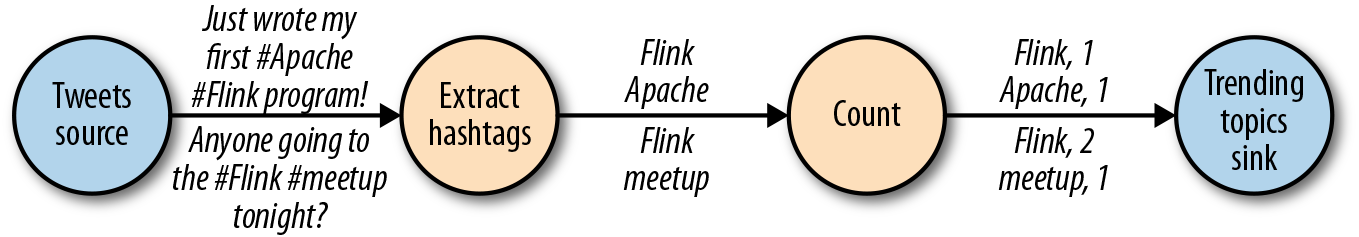
\includegraphics[width=0.7\textwidth]{images/spaf_0201.png}
  \caption{lambda架构}
\end{figure}

像上图中的数据流图被称为逻辑流图，因为它们表示了计算逻辑的高级视图。为了执行一个数据流程序，Flink会将逻辑流图转换为物理数据流图，详细说明程序的执行方式。例如，如果我们使用分布式处理引擎，每个算子在不同的物理机器可能有几个并行的任务运行。图2-2显示了图2-1逻辑图的物理数据流图。而在逻辑数据流图中节点表示算子，在物理数据流图中，节点是任务。“Extract hashtags”和“Count”算子有两个并行算子任务，每个算子任务对输入数据的子集执行计算。

\begin{figure}[htbp]
  \centering
  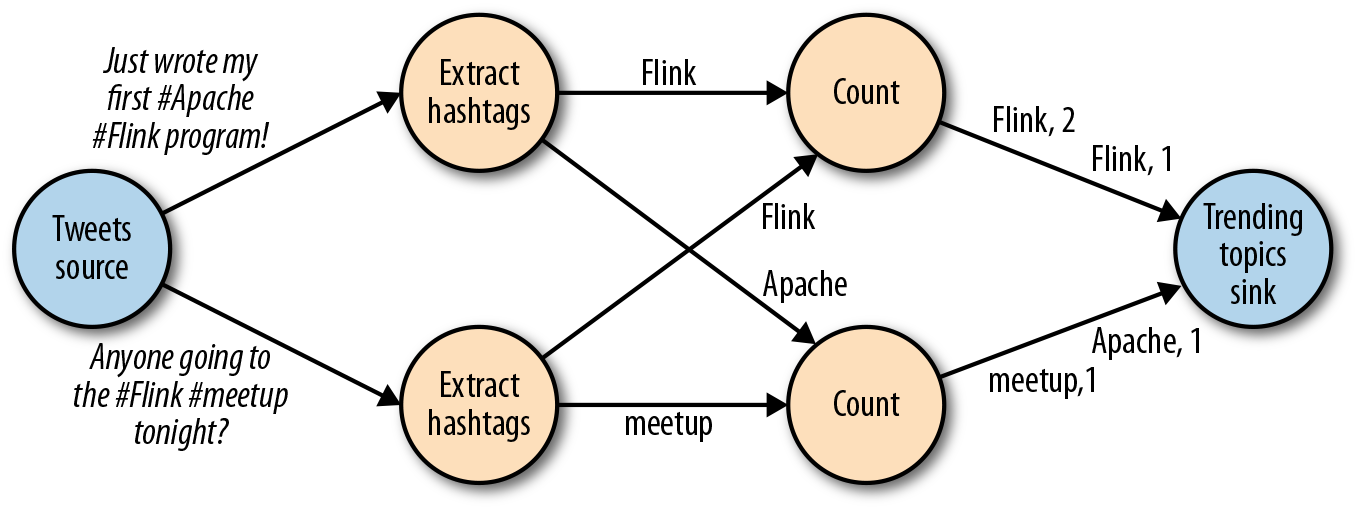
\includegraphics[width=0.7\textwidth]{images/spaf_0202.png}
  \caption{lambda架构}
\end{figure}

\subsection{数据并行和任务并行}

我们可以以不同方式利用数据流图中的并行性。第一，我们可以对输入数据进行分区，并在数据的子集上并行执行具有相同算子的任务并行。这种类型的并行性被称为数据并行性。数据并行是有用的，因为它允许处理大量数据，并将计算分散到不同的计算节点上。第二，我们可以将不同的算子在相同或不同的数据上并行执行。这种并行性称为任务并行性。使用任务并行性，我们可以更好地利用计算资源。

\subsection{数据交换策略}

数据交换策略定义了在物理执行流图中如何将数据分配给任务。数据交换策略可以由执行引擎自动选择，具体取决于算子的语义或我们明确指定的语义。在这里，我们简要回顾一些常见的数据交换策略，如图2-3所示。

\begin{figure}[htbp]
  \centering
  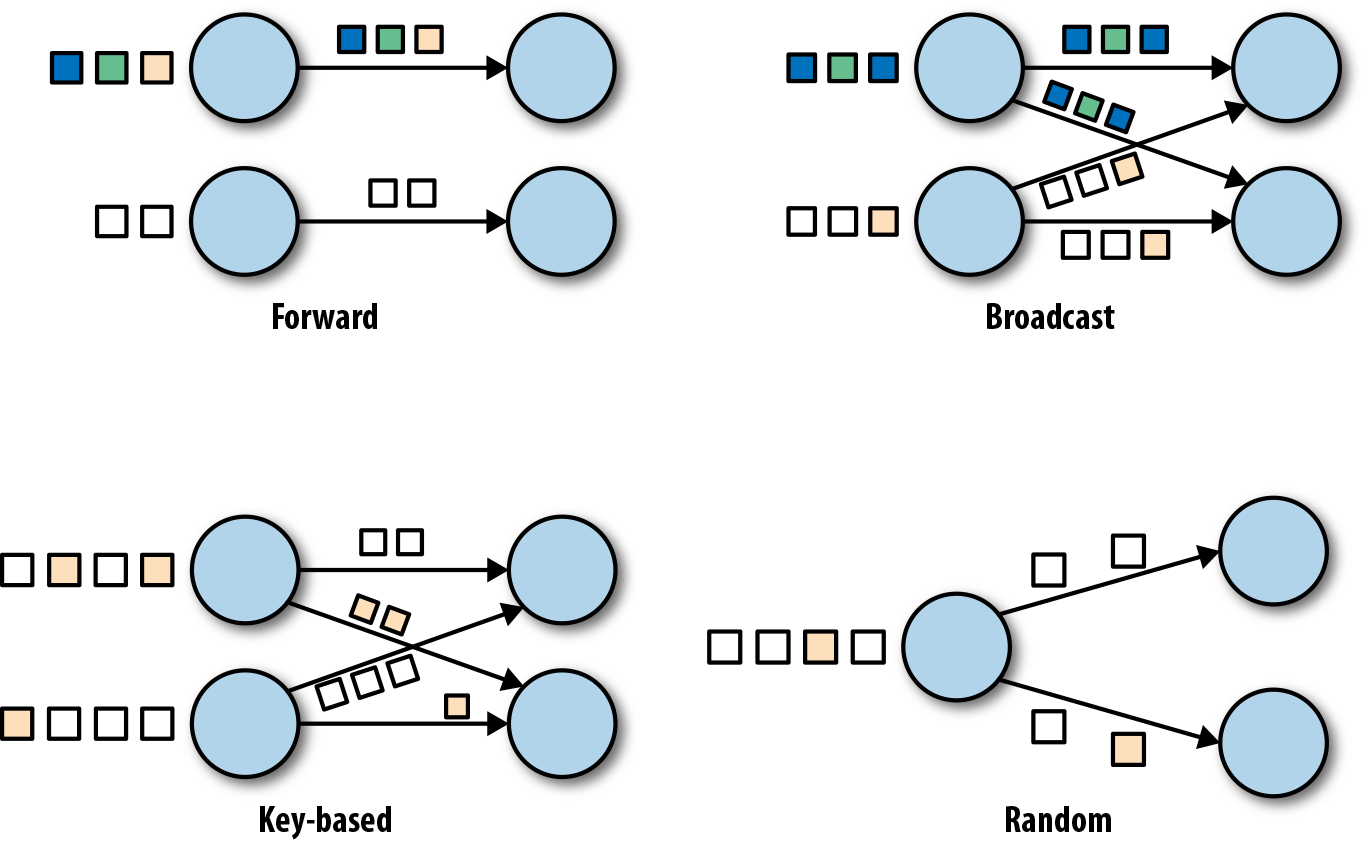
\includegraphics[width=0.7\textwidth]{images/spaf_0203.png}
  \caption{lambda架构}
\end{figure}

\begin{itemize}
    \item 前向策略将数据从一个任务发送到接收任务。如果两个任务都位于同一台物理计算机上（这通常由任务调度器确保），这种交换策略可以避免网络通信。
    \item 广播策略将所有数据发送到算子的所有的并行任务上面去。因为这种策略会复制数据和涉及网络通信，所以代价相当昂贵。
    \item 基于键控的策略通过Key值(键)对数据进行分区保证具有相同Key的数据将由同一任务处理。在图2-2中，输出“Extract hashtags”算子使用键来分区（hashtag），以便count算子的任务可以正确计算每个\#标签的出现次数。
    \item 随机策略统一将数据分配到算子的任务中去，以便均匀地将负载分配到不同的计算任务。
\end{itemize}

\section{并行处理流数据}

既然我们熟悉了数据流编程的基础知识，现在是时候看看这些概念如何应用于并行的处理数据流了。但首先，让我们定义术语数据流：数据流是一个可能无限的事件序列。

数据流中的事件可以表示监控数据，传感器测量数据，信用卡交易数据，气象站观测数据，在线用户交互数据，网络搜索数据等。在本节中，我们将学习如何并行处理无限流，使用数据流编程范式。

\subsection{延迟和吞吐量}

流处理程序不同与批处理程序。在评估性能时，要求也有所不同。对于批处理程序，我们通常关心一个作业的总的执行时间，或我们的处理引擎读取输入所需的时间，执行计算，并回写结果。由于流处理程序是连续运行的，输入可能是无界的，所以数据流处理中没有总执行时间的概念。 相反，流处理程序必须尽可能快的提供输入数据的计算结果。我们使用延迟和吞吐量来表征流处理的性能要求。

\subsection{延迟}

延迟表示处理事件所需的时间。它是接收事件和看到在输出中处理此事件的效果之间的时间间隔。要直观的理解延迟，考虑去咖啡店买咖啡。当你进入咖啡店时，可能还有其他顾客在里面。因此，你排队等候直到轮到你下订单。收银员收到你的付款并通知准备饮料的咖啡师。一旦你的咖啡准备好了，咖啡师会叫你的名字，你可以到柜台拿你的咖啡。服务延迟是从你进入咖啡店的那一刻起，直到你喝上第一口咖啡之间的时间间隔。

在数据流中，延迟是以时间为单位测量的，例如毫秒。根据应用程序，我们可能会关心平均延迟，最大延迟或百分位延迟。例如，平均延迟值为10ms意味着处理事件的平均时间在10毫秒内。或者，延迟值为95\%，10ms表示95\%的事件在10ms内处理完毕。平均值隐藏了处理延迟的真实分布，可能会让人难以发现问题。如果咖啡师在准备卡布奇诺之前用完了牛奶，你必须等到他们从供应室带来一些。虽然你可能会因为这么长时间的延迟而生气，但大多数其他客户仍然会感到高兴。

确保低延迟对于许多流应用程序来说至关重要，例如欺诈检测，系统警报，网络监控和提供具有严格服务水平协议的服务。低延迟是流处理的关键特性，它实现了我们所谓的实时应用程序。像Apache Flink这样的现代流处理器可以提供低至几毫秒的延迟。相比之下，传统批处理程序延迟通常从几分钟到几个小时不等。在批处理中，首先需要收集事件批次，然后才能处理它们。因此，延迟是受每个批次中最后一个事件的到达时间的限制。所以自然而然取决于批的大小。真正的流处理不会引入这样的人为延迟，因此可以实现真正的低延迟。真的流模型，事件一进入系统就可以得到处理。延迟更密切地反映了在每个事件上必须进行的实际工作。

\subsection{吞吐量}

吞吐量是衡量系统处理能力的指标，也就是处理速率。也就是说，吞吐量告诉我们每个时间单位系统可以处理多少事件。重温咖啡店的例子，如果商店营业时间为早上7点至晚上7点。当天为600个客户提供了服务，它的平均吞吐量将是每小时50个客户。虽然我们希望延迟尽可能低，但我们通常也需要吞吐量尽可能高。

吞吐量以每个时间单位系统所能处理的事件数量或操作数量来衡量。值得注意的是，事件处理速率取决于事件到达的速率，低吞吐量并不一定表示性能不佳。 在流式系统中，我们通常希望确保我们的系统可以处理最大的预期事件到达的速率。也就是说，我们主要的关注点在于确定的峰值吞吐量是多少，当系统处于最大负载时性能怎么样。为了更好地理解峰值吞吐量的概念，让我们考虑一个流处理 程序没有收到任何输入的数据，因此没有消耗任何系统资源。当第一个事件进来时，它会尽可能以最小延迟立即处理。例如，如果你是第一个出现在咖啡店的顾客，在早上开门后，你将立即获得服务。理想情况下，您希望此延迟保持不变 ，并且独立于传入事件的速率。但是，一旦我们达到使系统资源被完全使用的事件传入速率，我们将不得不开始缓冲事件。在咖啡店里 ，午餐后会看到这种情况发生。许多人出现在同一时间，必须排队等候。在此刻，咖啡店系统已达到其峰值吞吐量，进一步增加 事件传入的速率只会导致更糟糕的延迟。如果系统继续以可以处理的速率接收数据，缓冲区可能变为不可用，数据可能会丢失。这种情况是众所周知的 作为背压，有不同的策略来处理它。

\subsection{延迟与吞吐量的对比}

此时，应该清楚延迟和吞吐量不是独立指标。如果事件需要在处理流水线中待上很长时间，我们不能轻易确保高吞吐量。同样，如果系统容量很小，事件将被缓冲，而且必须等待才能得到处理。

让我们重温一下咖啡店的例子来阐明一下延迟和吞吐量如何相互影响。首先，应该清楚存在没有负载时的最佳延迟。也就是说，如果你是咖啡店的唯一客户，会很快得到咖啡。然而，在繁忙时期，客户将不得不排队等待，并且会有延迟增加。另一个影响延迟和吞吐量的因素是处理事件所花费的时间或为每个客户提供服务所花费的时间。想象一下，期间圣诞节假期，咖啡师不得不为每杯咖啡画圣诞老人。这意味着准备一杯咖啡需要的时间会增加，导致每个人花费 更多的时间在等待咖啡师画圣诞老人，从而降低整体吞吐量。

那么，你可以同时获得低延迟和高吞吐量吗？或者这是一个无望的努力？我们可以降低得到咖啡的延迟 ，方法是：聘请一位更熟练的咖啡师来准备咖啡。在高负载时，这种变化也会增加吞吐量，因为会在相同的时间内为更多的客户提供服务。 实现相同结果的另一种方法是雇用第二个咖啡师来利用并行性。这里的主要想法是降低延迟来增加吞吐量。当然，如果系统可以更快的执行操作，它可以在相同的时间内执行更多操作。 事实上，在流中利用并行性时也会发生这种情况。通过并行处理多个流，在同时处理更多事件的同时降低延迟。

\section{数据流上的操作}

流处理引擎通常提供一组内置操作：摄取(ingest)，转换(transform)和输出流(output)。这些操作可以 结合到数据流图中来实现逻辑流处理程序。在本节中，我们描述最常见的流处理操作。

操作可以是无状态的或有状态的。无状态操作不保持任何内部状态。也就是说，事件的处理不依赖于过去看到的任何事件，也没有保留历史。 无状态操作很容易并行化，因为事件可以彼此独立地处理，也独立于事件到达的顺序(和事件到达顺序没有关系)。 而且，在失败的情况下，无状态操作可以是简单的重新启动并从中断处继续处理。相反， 有状态操作可能会维护之前收到的事件的信息。此状态可以通过传入事件更新，也可以用于未来事件的处理逻辑。有状态的流 处理应用程序更难以并行化和以容错的方式来运行，因为状态需要有效的进行分区和在发生故障的情况下可靠地恢复。

\subsection{数据摄入和数据吞吐量}

数据摄取和数据出口操作允许流处理程序与外部系统通信。数据摄取是操作从外部源获取原始数据并将其转换为其他格式(ETL)。实现数据提取逻辑的运算符被称为数据源。数据源可以从TCP Socket，文件，Kafka Topic或传感器数据接口中提取数据。数据出口是以适合消费的形式产出到外部系统。执行数据出口的运算符称为数据接收器，包括文件，数据库，消息队列和监控接口。

\subsection{转换算子}

\begin{figure}[htbp]
  \centering
  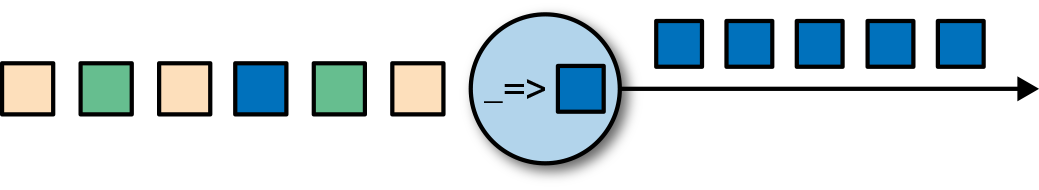
\includegraphics[width=0.7\textwidth]{images/spaf_0204.png}
  \caption{lambda架构}
\end{figure}

转换算子是单遍处理算子，碰到一个事件处理一个事件。这些操作在使用后会消费一个事件，然后对事件数据做一些转换，产生一个新的输出流。转换逻辑可以集成在 操作符中或由UDF函数提供，如图所示图2-4。程序员编写实现自定义计算逻辑。

操作符可以接受多个输入流并产生多个输出流。他们还可以通过修改数据流图的结构要么将流分成多个流，要么将流合并为一条流。

\subsection{滚动聚合}

滚动聚合是一种聚合，例如sum，minimum和maximum，为每个输入事件不断更新。 聚合操作是有状态的，并将当前状态与传入事件一起计算以产生更新的聚合值。请注意能够有效地将当前状态与事件相结合 产生单个值，聚合函数必须是关联的和可交换的。否则，操作符必须存储完整的流数据历史。图2-5显示了最小滚动 聚合。操作符保持当前的最小值和相应地为每个传入的事件来更新最小值。

\begin{figure}[htbp]
  \centering
  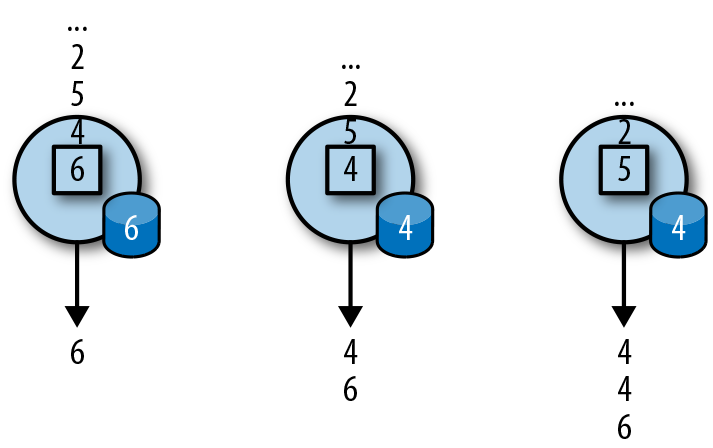
\includegraphics[width=0.7\textwidth]{images/spaf_0205.png}
  \caption{lambda架构}
\end{figure}

\subsection{窗口操作符}

转换和滚动聚合一次处理一个事件产生输出事件并可能更新状态。但是，有些操作必须收集并缓冲数据以计算其结果。 例如，考虑不同流之间的连接或整体聚合这样的操作，例如中值函数。为了在无界流上高效运行这些操作符，我们需要限制 这些操作维护的数据量。在本节中，我们将讨论窗口操作，提供此服务。

窗口还可以在语义上实现关于流的比较复杂的查询。我们已经看到了滚动聚合的方式，以聚合值编码整个流的历史数据来为每个事件提供低延迟的结果。 但如果我们只对最近的数据感兴趣的话会怎样？考虑给司机提供实时交通信息的应用程序。这个程序可以使他们避免拥挤的路线。在这种场景下，你想知道某个位置在最近几分钟内是否有事故发生。 另一方面，了解所有发生过的事故在这个应用场景下并没有什么卵用。更重要的是，通过将流历史缩减为单一聚合值，我们将丢失这段时间内数据的变化。例如，我们可能想知道每5分钟有多少车辆穿过 某个路口。

窗口操作不断从无限事件流中创建有限的事件集，好让我们执行有限集的计算。通常会基于数据属性或基于时间的窗口来分配事件。 要正确定义窗口运算符语义，我们需要确定如何给窗口分配事件以及对窗口中的元素进行求值的频率是什么样的。 窗口的行为由一组策略定义。窗口策略决定何时创建新的窗口以及要分配的事件属于哪个窗口，以及何时对窗口中的元素进行求值。 而窗口的求值基于触发条件。一旦触发条件得到满足，窗口的内容将会被发送到求值函数，求值函数会将计算逻辑应用于窗口中的元素。 求值函数可以是sum或minimal或自定义的聚合函数。 求值策略可以根据时间或者数据属性计算(例如，在过去五秒内收到的事件或者最近的一百个事件等等)。 接下来，我们描述常见窗口类型的语义。

\begin{itemize}
    \item 滚动窗口是将事件分配到固定大小的不重叠的窗口中。当通过窗口的结尾时，全部事件被发送到求值函数进行处理。基于计数的滚动窗口定义了在触发求值之前需要收集多少事件。图2-6显示了一个基于计数的翻滚窗口，每四个元素一个窗口。基于时间的滚动窗口定义一个时间间隔，包含在此时间间隔内的事件。图2-7显示了基于时间的滚动窗口，将事件收集到窗口中每10分钟触发一次计算。
        \begin{figure}[htbp]
          \centering
          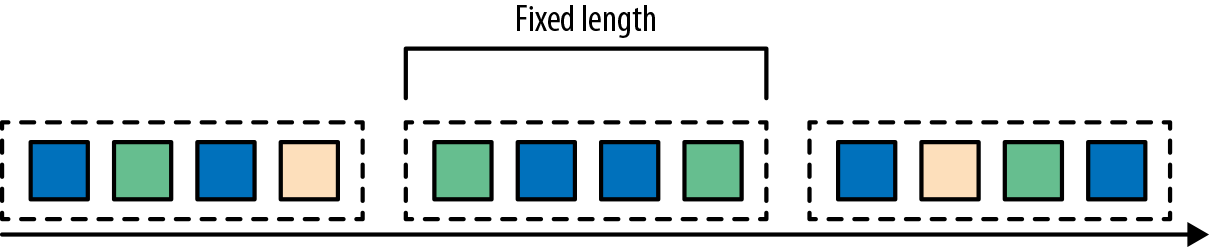
\includegraphics[width=0.7\textwidth]{images/spaf_0206.png}
          \caption{lambda架构}
        \end{figure}
        \begin{figure}[htbp]
          \centering
          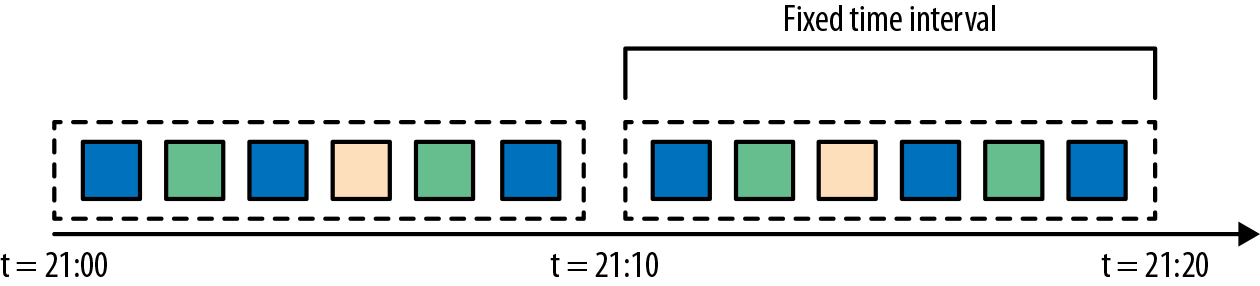
\includegraphics[width=0.7\textwidth]{images/spaf_0207.png}
          \caption{lambda架构}
        \end{figure}
    \item 滑动窗口将事件分配到固定大小的重叠的窗口中去。因此，事件可能属于多个桶。我们通过提供窗口的长度和滑动距离来定义滑动窗口。滑动距离定义了创建新窗口的间隔。基于滑动计数的窗口，图2-8的长度为四个事件，三个为滑动距离。
        \begin{figure}[htbp]
          \centering
          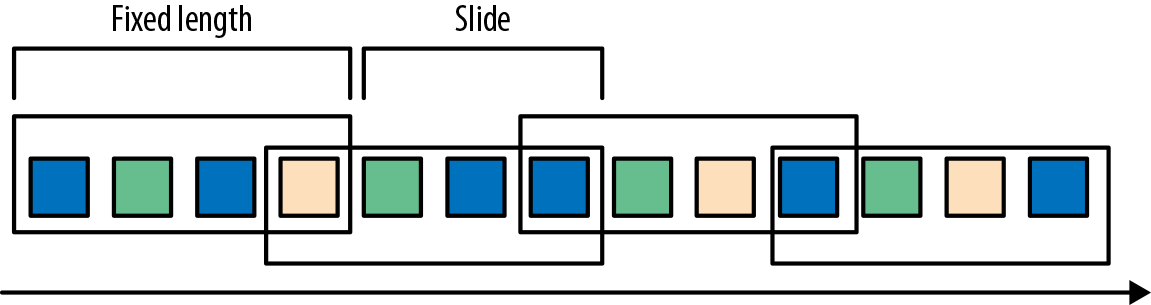
\includegraphics[width=0.7\textwidth]{images/spaf_0208.png}
          \caption{lambda架构}
        \end{figure}
    \item 会话窗口在常见的真实场景中很有用，一些场景既不能使用滚动窗口也不能使用滑动窗口。考虑一个分析在线用户行为的应用程序。在应用程序里，我们想把源自同一时期的用户活动或会话事件分组在一起。会话由一系列相邻时间发生的事件组成，接下来有一段时间没有活动。例如，用户在App上浏览一系列的新闻，然后关掉App，那么浏览新闻这段时间的浏览事件就是一个会话。会话窗口事先没有定义窗口的长度，而是取决于数据的实际情况，滚动窗口和滑动窗口无法应用于这个场景。相反，我们需要将同一会话中的事件分配到同一个窗口中去，而不同的会话可能窗口长度不一样。会话窗口会定义一个间隙值来区分不同的会话。间隙值的意思是：用户一段时间内不活动，就认为用户的会话结束了。图2-9显示了一个会话窗口。
        \begin{figure}[htbp]
          \centering
          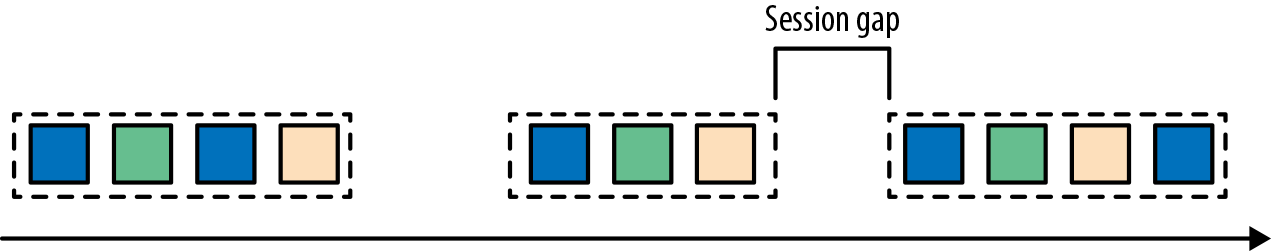
\includegraphics[width=0.7\textwidth]{images/spaf_0209.png}
          \caption{lambda架构}
        \end{figure}
\end{itemize}

到目前为止，所有窗口类型都是在整条流上去做窗口操作。但实际上你可能想要将一条流分流成多个逻辑流并定义并行窗口。 例如，如果我们正在接收来自不同传感器的测量结果，那么可能想要在做窗口计算之前按传感器ID对流进行分流操作。 在并行窗口中，每条流都独立于其他流，然后应用了窗口逻辑。图2-10显示了一个基于计数的长度为2的并行滚动窗口，根据事件颜色分流。

\begin{figure}[htbp]
    \centering
    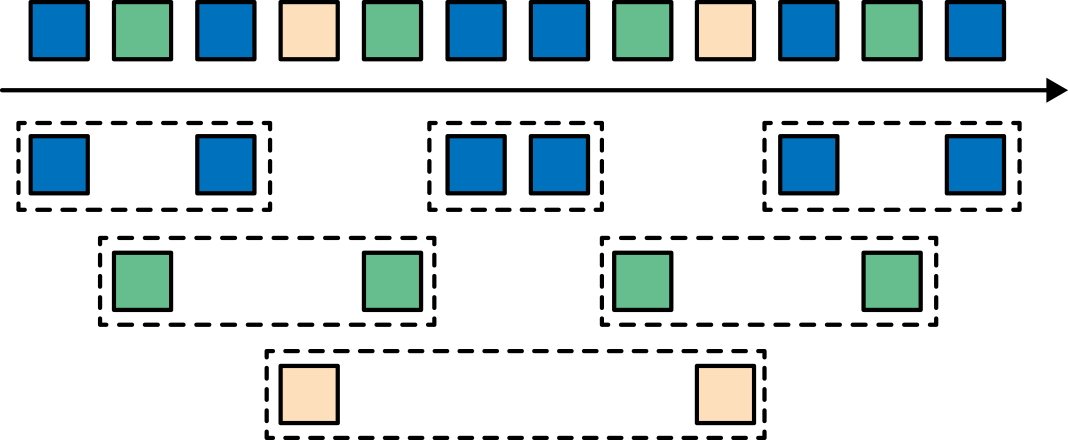
\includegraphics[width=0.7\textwidth]{images/spaf_0210.png}
    \caption{lambda架构}
\end{figure}

在流处理中，窗口操作与两个主要概念密切相关：时间语义和状态管理。时间也许是流处理最重要的方面。即使低延迟是流处理的一个有吸引力的特性，它的真正价值不仅仅是快速分析。真实世界的系统，网络和通信渠道远非完美，流数据经常被推迟或无序(乱序)到达。理解如何在这种条件下提供准确和确定的结果是至关重要的。 更重要的是，流处理程序可以按原样处理事件制作的也应该能够处理相同的历史事件方式，从而实现离线分析甚至时间旅行分析。 当然，前提是我们的系统可以保存状态，因为可能有故障发生。到目前为止，我们看到的所有窗口类型在产生结果前都需要保存之前的数据。实际上，如果我们想计算任何指标，即使是简单的计数，我们也需要保存状态。考虑到流处理程序可能会运行几天，几个月甚至几年，我们需要确保状态可以在发生故障的情况下可靠地恢复。 并且即使程序崩溃，我们的系统也能保证计算出准确的结果。本章，我们将在流处理应用可能发生故障的语境下，深入探讨时间和状态的概念。

\section{时间语义}

在本节中，我们将介绍时间语义，并描述流中不同的时间概念。我们将讨论流处理器在乱序事件流的情况下如何提供准确的计算结果，以及我们如何处理历史事件流，如何在流中进行时间旅行。

\subsection{在流处理中一分钟代表什么？}

在处理可能是无限的事件流（包含了连续到达的事件），时间成为流处理程序的核心方面。假设我们想要连续的计算结果，可能每分钟就要计算一次。在我们的流处理程序上下文中，一分钟的意思是什么？

考虑一个程序需要分析一款移动端的在线游戏的用户所产生的事件流。游戏中的用户分了组，而应用程序将收集每个小组的活动数据，基于小组中的成员多快达到了游戏设定的目标，然后在游戏中提供奖励。例如额外的生命和用户升级。例如，如果一个小组中的所有用户在一分钟之内都弹出了500个泡泡，他们将升一级。Alice是一个勤奋的玩家，她在每天早晨的通勤时间玩游戏。问题在于Alice住在柏林，并且乘地铁去上班。而柏林的地铁手机信号很差。我们设想一个这样的场景，Alice当她的手机连上网时，开始弹泡泡，然后游戏会将数据发送到我们编写的应用程序中，这时地铁突然进入了隧道，她的手机也断网了。Alice还在玩这个游戏，而产生的事件将会缓存在手机中。当地铁离开隧道，Alice的手机又在线了，而手机中缓存的游戏事件将发送到应用程序。我们的应用程序应该如何处理这些数据？在这个场景中一分钟的意思是什么？这个一分钟应该包含Alice离线的那段时间吗？下图展示了这个问题。

\begin{figure}[htbp]
    \centering
    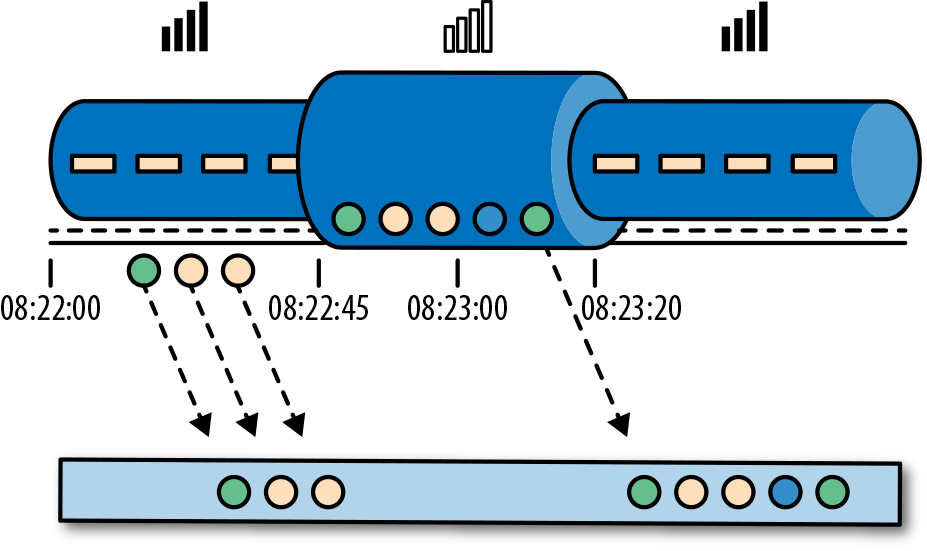
\includegraphics[width=0.7\textwidth]{images/spaf_0211.png}
    \caption{lambda架构}
\end{figure}

在线手游是一个简单的场景，展示了应用程序的运算应该取决于事件实际发生的时间，而不是应用程序收到事件的时间。如果我们按照应用程序收到事件的时间来进行处理的话，最糟糕的后果就是，Alice和她的朋友们再也不玩这个游戏了。但是还有很多时间语义非常关键的应用程序，我们需要保证时间语义的正确性。如果我们只考虑我们在一分钟之内收到了多少数据，我们的结果会变化，因为结果取决于网络连接的速度或处理的速度。相反，定义一分钟之内的事件数量，这个一分钟应该是数据本身的时间。

在Alice的这个例子中，流处理程序可能会碰到两个不同的时间概念：处理时间和事件时间。我们将在接下来的部分，讨论这两个概念。

\subsection{处理时间}

处理时间是处理流的应用程序的机器的本地时钟的时间（墙上时钟）。处理时间的窗口包含了一个时间段内来到机器的所有事件。这个时间段指的是机器的墙上时钟。如下图所示，在Alice的这个例子中，处理时间窗口在Alice的手机离线的情况下，时间将会继续行走。但这个处理时间窗口将不会收集Alice的手机离线时产生的事件。

\begin{figure}[htbp]
    \centering
    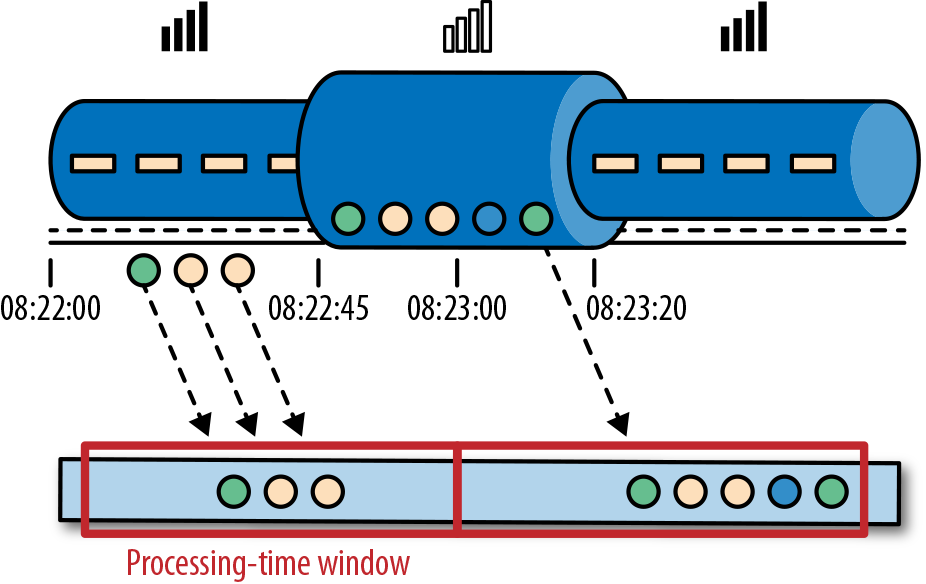
\includegraphics[width=0.7\textwidth]{images/spaf_0212.png}
    \caption{lambda架构}
\end{figure}

\subsection{事件时间}

事件时间是流中的事件实际发生的时间。事件时间基于流中的事件所包含的时间戳。通常情况下，在事件进入流处理程序前，事件数据就已经包含了时间戳。下图展示了事件时间窗口将会正确的将事件分发到窗口中去。可以如实反应事情是怎么发生的。即使事件可能存在延迟。

\begin{figure}[htbp]
    \centering
    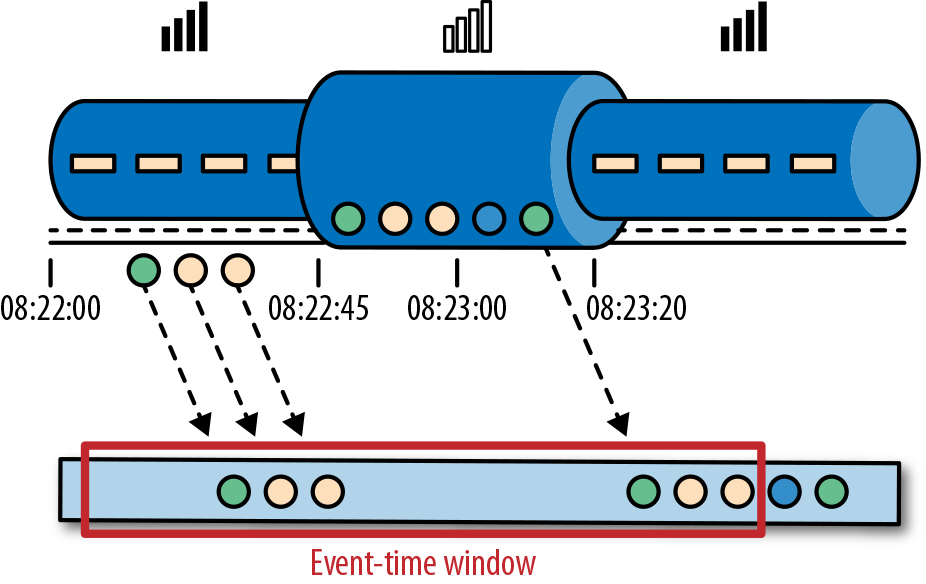
\includegraphics[width=0.7\textwidth]{images/spaf_0213.png}
    \caption{lambda架构}
\end{figure}

事件时间使得计算结果的过程不需要依赖处理数据的速度。基于事件时间的操作是可以预测的，而计算结果也是确定的。无论流处理程序处理流数据的速度快或是慢，无论事件到达流处理程序的速度快或是慢，事件时间窗口的计算结果都是一样的。

可以处理迟到的事件只是我们使用事件时间所克服的一个挑战而已。普遍存在的事件乱序问题可以使用事件时间得到解决。考虑和Alice玩同样游戏的Bob，他恰好和Alice在同一趟地铁上。Alice和Bob虽然玩的游戏一样，但他们的手机信号是不同的运营商提供的。当Alice的手机没信号时，Bob的手机依然有信号，游戏数据可以正常发送出去。

如果使用事件时间，即使碰到了事件乱序到达的情况，我们也可以保证结果的正确性。还有，当我们在处理可以重播的流数据时，由于时间戳的确定性，我们可以快进过去。也就是说，我们可以重播一条流，然后分析历史数据，就好像流中的事件是实时发生一样。另外，我们可以快进历史数据来使我们的应用程序追上现在的事件，然后应用程序仍然是一个实时处理程序，而且业务逻辑不需要改变。

\subsection{水位线}

在我们对事件时间窗口的讨论中，我们忽略了一个很重要的方面：我们应该怎样去决定何时触发事件时间窗口的计算？也就是说，在我们可以确定一个时间点之前的所有事件都已经到达之前，我们需要等待多久？我们如何知道事件是迟到的？在分布式系统无法准确预测行为的现实条件下，以及外部组件所引发的事件的延迟，以上问题并没有准确的答案。在本小节中，我们将会看到如何使用水位线来设置事件时间窗口的行为。

水位线是全局进度的度量标准。系统可以确信在一个时间点之后，不会有早于这个时间点发生的事件到来了。本质上，水位线提供了一个逻辑时钟，这个逻辑时钟告诉系统当前的事件时间。当一个运算符接收到含有时间T的水位线时，这个运算符会认为早于时间T的发生的事件已经全部都到达了。对于事件时间窗口和乱序事件的处理，水位线非常重要。运算符一旦接收到水位线，运算符会认为一段时间内发生的所有事件都已经观察到，可以触发针对这段时间内所有事件的计算了。

水位线提供了一种结果可信度和延时之间的妥协。激进的水位线设置可以保证低延迟，但结果的准确性不够。在这种情况下，迟到的事件有可能晚于水位线到达，我们需要编写一些代码来处理迟到事件。另一方面，如果水位线设置的过于宽松，计算的结果准确性会很高，但可能会增加流处理程序不必要的延时。

在很多真实世界的场景里面，系统无法获得足够的知识来完美的确定水位线。在手游这个场景中，我们无法得知一个用户离线时间会有多长，他们可能正在穿越一条隧道，可能正在乘飞机，可能永远不会再玩儿了。水位线无论是用户自定义的或者是自动生成的，在一个分布式系统中追踪全局的时间进度都不是很容易。所以仅仅依靠水位线可能并不是一个很好的主意。流处理系统还需要提供一些机制来处理迟到的元素（在水位线之后到达的事件）。根据应用场景，我们可能需要把迟到事件丢弃掉，或者写到日志里，或者使用迟到事件来更新之前已经计算好的结果。

\subsection{处理时间和事件时间}

大家可能会有疑问，既然事件时间已经可以解决我们的所有问题，为什么我们还要对比这两个时间概念？真相是，处理时间在很多情况下依然很有用。处理时间窗口将会带来理论上最低的延迟。因为我们不需要考虑迟到事件以及乱序事件，所以一个窗口只需要简单的缓存窗口内的数据即可，一旦机器时间超过指定的处理时间窗口的结束时间，就会触发窗口的计算。所以对于一些处理速度比结果准确性更重要的流处理程序，处理时间就派上用场了。另一个应用场景是，当我们需要在真实的时间场景下，周期性的报告结果时，同时不考虑结果的准确性。一个例子就是一个实时监控的仪表盘，负责显示当事件到达时立即聚合的结果。最后，处理时间窗口可以提供流本身数据的忠实表达，对于一些案例可能是很必要的特性。例如我们可能对观察流和对每分钟事件的计数（检测可能存在的停电状况）很感兴趣。简单的说，处理时间提供了低延迟，同时结果也取决于处理速度，并且也不能保证确定性。另一方面，事件时间保证了结果的确定性，同时还可以使我们能够处理迟到的或者乱序的事件流。

\section{状态和持久化模型}

我们现在转向另一个对于流处理程序非常重要的话题：状态。在数据处理中，状态是普遍存在的。任何稍微复杂一点的计算，都涉及到状态。为了产生计算结果，一个函数在一段时间内的一定数量的事件上来累加状态（例如，聚合计算或者模式匹配）。有状态的运算符使用输入的事件以及内部保存的状态来计算得到输出。例如，一个滚动聚合运算符需要输出这个运算符所观察到的所有事件的累加和。这个运算符将会在内部保存当前观察到的所有事件的累加和，同时每输入一个事件就更新一次累加和的计算结果。相似的，当一个运算符检测到一个“高温”事件紧接着十分钟以内检测到一个“烟雾”事件时，将会报警。直到运算符观察到一个“烟雾”事件或者十分钟的时间段已经过去，这个运算符需要在内部状态中一直保存着“高温”事件。

当我们考虑一下使用批处理系统来分析一个无界数据集时，会发现状态的重要性显而易见。在现代流处理器兴起之前，处理无界数据集的一个通常做法是将输入的事件攒成微批，然后交由批处理器来处理。当一个任务结束时，计算结果将被持久化，而所有的运算符状态就丢失了。一旦一个任务在计算下一个微批次的数据时，这个任务是无法访问上一个任务的状态的（都丢掉了）。这个问题通常使用将状态代理到外部系统（例如数据库）的方法来解决。相反，在一个连续不间断运行的流处理任务中，事件的状态是一直存在的，我们可以将状态暴露出来作为编程模型中的一等公民。当然，我们的确可以使用外部系统来管理流的状态，即使这个解决方案会带来额外的延迟。

由于流处理运算符默认处理的是无界数据流。所以我们必须要注意不要让内部状态无限的增长。为了限制状态的大小，运算符通常情况下会保存一些之前所观察到的事件流的总结或者概要。这个总结可能是一个计数值，一个累加和，或者事件流的采样，窗口的缓存操作，或者是一个自定义的数据结构，这个数据结构用来保存数据流中感兴趣的一些特性。

我们可以想象的到，支持有状态的运算符可能会碰到一些实现上的挑战：

\begin{itemize}
    \item 状态管理：系统需要高效的管理状态，并保证针对状态的并发更新，不会产生竞争条件（race condition）。
    \item 状态分区：并行会带来复杂性。因为计算结果同时取决于已经保存的状态和输入的事件流。幸运的是，大多数情况下，我们可以使用Key来对状态进行分区，然后独立的管理每一个分区。例如，当我们处理一组传感器的测量事件流时，我们可以使用分区的运算符状态来针对不同的传感器独立的保存状态。
    \item 状态恢复：第三个挑战是有状态的运算符如何保证状态可以恢复，即使出现任务失败的情况，计算也是正确的。
\end{itemize}

下一节，我们将讨论任务失败和计算结果的保证。

\subsection{任务失败}

流任务中的运算符状态是很宝贵的，也需要抵御任务失败带来的问题。如果在任务失败的情况下，状态丢失的话，在任务恢复以后计算的结果将是不正确的。流任务会连续不断的运行很长时间，而状态可能已经收集了几天甚至几个月。在失败的情况下，重新处理所有的输入并重新生成一个丢失的状态，将会很浪费时间，开销也很大。

在本章开始时，我们看到如何将流的编程建模成数据流模型。在执行之前，流程序将会被翻译成物理层数据流图，物理层数据流图由连接的并行任务组成，而一个并行任务运行一些运算符逻辑，消费输入流数据，并为其他任务产生输出流数据。真实场景下，可能有数百个这样的任务并行运行在很多的物理机器上。在长时间的运行中，流任务中的任意一个任务在任意时间点都有可能失败。我们如何保证任务的失败能被正确的处理，以使任务能继续的运行下去呢？事实上，我们可能希望我们的流处理器不仅能在任务失败的情况下继续处理数据，还能保证计算结果的正确性以及运算符状态的安全。我们在本小节来讨论这些问题。

\textbf{什么是任务失败？}

对于流中的每一个事件，一个处理任务分为以下步骤：（1）接收事件，并将事件存储在本地的缓存中；（2）可能会更新内部状态；（3）产生输出记录。这些步骤都能失败，而系统必须对于在失败的场景下如何处理有清晰的定义。如果任务在第一步就失败了，事件会丢失吗？如果当更新内部状态的时候任务失败，那么内部状态会在任务恢复以后更新吗？在以上这些场景中，输出是确定性的吗？

在批处理场景下，所有的问题都不是问题。因为我们可以很方便的重新计算。所以不会有事件丢失，状态也可以得到完全恢复。在流的世界里，处理失败不是一个小问题。流系统在失败的情况下需要保证结果的准确性。接下来，我们需要看一下现代流处理系统所提供的一些保障，以及实现这些保障的机制。

\textbf{结果的保证}

当我们讨论保证计算的结果时，我们的意思是流处理器的内部状态需要保证一致性。也就是说我们关心的是应用程序的代码在故障恢复以后看到的状态值是什么。要注意保证应用程序状态的一致性并不是保证应用程序的输出结果的一致性。一旦输出结果被持久化，结果的准确性就很难保证了。除非持久化系统支持事务。

\textit{AT-MOST-ONCE}

当任务故障时，最简单的做法是什么都不干，既不恢复丢失的状态，也不重播丢失的事件。At-most-once语义的含义是最多处理一次事件。换句话说，事件可以被丢弃掉，也没有任何操作来保证结果的准确性。这种类型的保证也叫“没有保证”，因为一个丢弃掉所有事件的系统其实也提供了这样的保障。没有保障听起来是一个糟糕的主意，但如果我们能接受近似的结果，并且希望尽可能低的延迟，那么这样也挺好。

\textit{AT-LEAST-ONCE}

在大多数的真实应用场景，我们希望不丢失事件。这种类型的保障成为at-least-once，意思是所有的事件都得到了处理，而且一些事件还可能被处理多次。如果结果的正确性仅仅依赖于数据的完整性，那么重复处理是可以接受的。例如，判断一个事件是否在流中出现过，at-least-once这样的保证完全可以正确的实现。在最坏的情况下，我们多次遇到了这个事件。而如果我们要对一个特定的事件进行计数，计算结果就可能是错误的了。

为了保证在at-least-once语义的保证下，计算结果也能正确。我们还需要另一套系统来从数据源或者缓存中重新播放数据。持久化的事件日志系统将会把所有的事件写入到持久化存储中。所以如果任务发生故障，这些数据可以重新播放。还有一种方法可以获得同等的效果，就是使用结果承认机制。这种方法将会把每一条数据都保存在缓存中，直到数据的处理等到所有的任务的承认。一旦得到所有任务的承认，数据将被丢弃。

\textit{EXACTLY-ONCE}

恰好处理一次是最严格的保证，也是最难实现的。恰好处理一次语义不仅仅意味着没有事件丢失，还意味着针对每一个数据，内部状态仅仅更新一次。本质上，恰好处理一次语义意味着我们的应用程序可以提供准确的结果，就好像从未发生过故障。

提供恰好处理一次语义的保证必须有至少处理一次语义的保证才行，同时还需要数据重放机制。另外，流处理器还需要保证内部状态的一致性。也就是说，在故障恢复以后，流处理器应该知道一个事件有没有在状态中更新。事务更新是达到这个目标的一种方法，但可能引入很大的性能问题。Flink使用了一种轻量级快照机制来保证恰好处理一次语义。

\textit{端到端恰好处理一次}

目前我们看到的一致性保证都是由流处理器实现的，也就是说都是在Flink流处理器内部保证的。而在真实世界中，流处理应用除了流处理器以外还包含了数据源（例如Kafka）和持久化系统。端到端的一致性保证意味着结果的正确性贯穿了整个流处理应用的始终。每一个组件都保证了它自己的一致性。而整个端到端的一致性级别取决于所有组件中一致性最弱的组件。要注意的是，我们可以通过弱一致性来实现更强的一致性语义。例如，当任务的操作具有幂等性时，比如流的最大值或者最小值的计算。在这种场景下，我们可以通过最少处理一次这样的一致性来实现恰好处理一次这样的最高级别的一致性。

\chapter{Flink运行架构}

\section{系统架构}

Flink是一个用于有状态的并行数据流处理的分布式系统。它由多个进程构成，这些进程一般会分布运行在不同的机器上。对于分布式系统来说，面对的常见问题有：集群中资源的分配和管理、进程协调调度、持久化和高可用的数据存储，以及故障恢复。

对于这些分布式系统的经典问题，业内已有比较成熟的解决方案和服务。所以Flink并不会自己去处理所有的问题，而是利用了现有的集群架构和服务，这样它就可以把精力集中在核心工作——分布式数据流处理上了。Flink与一些集群资源管理工具有很好的集成，比如Apache Mesos、YARN和Kubernetes；同时，也可以配置为独立（stand-alone）集群运行。Flink自己并不提供持久化的分布式存储，而是直接利用了已有的分布式文件系统（比如HDFS）或者对象存储（比如S3）。对于高可用的配置，Flink需要依靠Apache ZooKeeper来完成。

在本节中，我们将介绍Flink的不同组件，以及在运行程序时它们如何相互作用。我们会讨论部署Flink应用程序的两种模式，并且了解每种模式下分发和执行任务的方式。最后，我们还会解释一下Flink的高可用性模式是如何工作的。

\subsection{Flink运行时组件}

Flink运行时架构主要包括四个不同的组件，它们会在运行流处理应用程序时协同工作：作业管理器（JobManager）、资源管理器（ResourceManager）、任务管理器（TaskManager），以及分发器（Dispatcher）。因为Flink是用Java和Scala实现的，所以所有组件都会运行在Java虚拟机（JVMs）上。每个组件的职责如下：

\begin{itemize}
    \item 作业管理器（JobManager）是控制一个应用程序执行的主进程，也就是说，每个应用程序都会被一个不同的作业管理器所控制执行。作业管理器会先接收到要执行的应用程序。这个应用程序会包括：作业图（JobGraph）、逻辑数据流图（logical dataflow graph）和打包了所有的类、库和其它资源的JAR包。作业管理器会把JobGraph转换成一个物理层面的数据流图，这个图被叫做“执行图”（ExecutionGraph），包含了所有可以并发执行的任务。作业管理器会向资源管理器（ResourceManager）请求执行任务必要的资源，也就是任务管理器（TaskManager）上的插槽（slot）。一旦它获取到了足够的资源，就会将执行图分发到真正运行它们的TaskManager上。而在运行过程中，作业管理器会负责所有需要中央协调的操作，比如说检查点（checkpoints）的协调。
    \item ResourceManager主要负责管理任务管理器（TaskManager）的插槽（slot），TaskManger插槽是Flink中定义的处理资源单元。Flink为不同的环境和资源管理工具提供了不同资源管理器（ResourceManager），比如YARN、Mesos、K8s，以及standalone部署。当作业管理器申请插槽资源时，ResourceManager会将有空闲插槽的TaskManager分配给作业管理器。如果ResourceManager没有足够的插槽来满足作业管理器的请求，它还可以向资源提供平台发起会话，以提供启动TaskManager进程的容器。另外，ResourceManager还负责终止空闲的TaskManager，释放计算资源。
    \item 任务管理器（TaskManager）是Flink中的工作进程。通常在Flink中会有多个TaskManager运行，每一个TaskManager都包含了一定数量的插槽（slots）。插槽的数量限制了TaskManager能够执行的任务数量。启动之后，TaskManager会向资源管理器注册它的插槽；收到资源管理器的指令后，TaskManager就会将一个或者多个插槽提供给作业管理器调用。作业管理器就可以向插槽分配任务（tasks）来执行了。在执行过程中，一个TaskManager可以跟其它运行同一应用程序的TaskManager交换数据。任务的执行和插槽的概念会在“任务执行”一节做具体讨论。
    \item 分发器（Dispatcher）可以跨作业运行，它为应用提交提供了REST接口。当一个应用被提交执行时，分发器就会启动并将应用移交给一个作业管理器。由于是REST接口，所以Dispatcher可以作为集群的一个HTTP接入点，这样就能够不受防火墙阻挡。Dispatcher也会启动一个Web UI，用来方便地展示和监控作业执行的信息。Dispatcher在架构中可能并不是必需的，这取决于应用提交运行的方式。
\end{itemize}

\begin{figure}[htbp]
    \centering
    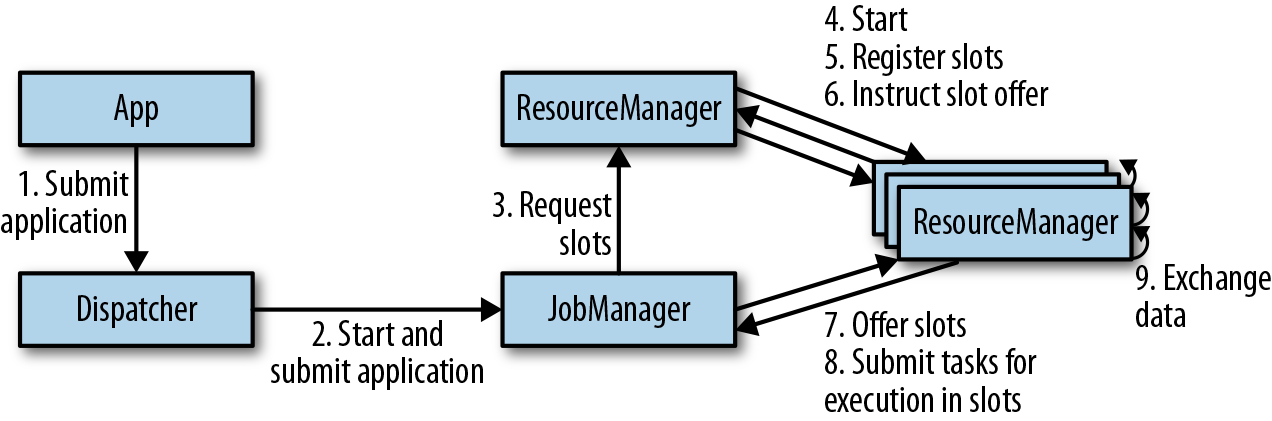
\includegraphics[width=0.7\textwidth]{images/spaf_0301.png}
    \caption{lambda架构}
\end{figure}

\begin{note}
    上图是从一个较为高层级的视角，来看应用中各组件的交互协作。如果部署的集群环境不同（例如YARN，Mesos，Kubernetes，standalone等），其中一些步骤可以被省略，或是有些组件会运行在同一个JVM进程中。
\end{note}

\subsection{应用部署}

Flink应用程序可以用以下两种不同的方式部署：

\textit{框架（Framework）方式}

在这个模式下，Flink应用被打包成一个Jar文件，并由客户端提交给一个运行服务（running service）。这个服务可以是一个Flink的Dispatcher，也可以是一个Flink的作业管理器，或是Yarn的ResourceManager。如果application被提交给一个作业管理器，则它会立即开始执行这个application。如果application被提交给了一个Dispatcher，或是Yarn ResourceManager，则它会启动一个作业管理器，然后将application交给它，再由作业管理器开始执行此应用。

\textit{库（Library）方式}

在这个模式下，Flink Application 会被打包在一个容器（container） 镜像里，例如一个Docker 镜像。此镜像包含了运行作业管理器和ResourceManager的代码。当一个容器从镜像启动后，它会自动启动ResourceManager和作业管理器，并提交打包好的应用。另一种方法是：将应用打包到镜像后，只用于部署TaskManager容器。从镜像启动的容器会自动启动一个TaskManager，然后连接ResourceManager并注册它的slots。这些镜像的启动以及失败重启，通常都会由一个外部的资源管理器管理（比如Kubernetes）。

框架模式遵循了传统的任务提交方式，从客户端提交到Flink运行服务。而在库模式下，没有运行的Flink服务。它是将Flink作为一个库，与应用程序一同打包到了一个容器镜像。这种部署方式在微服务架构中较为常见。我们会在“运行管理流式应用程序”一节对这个话题做详细讨论。

\subsection{任务执行}

一个TaskManager可以同时执行多个任务（tasks）。这些任务可以是同一个算子（operator）的子任务（数据并行），也可以是来自不同算子的（任务并行），甚至可以是另一个不同应用程序的（作业并行）。TaskManager提供了一定数量的处理插槽（processing slots），用于控制可以并行执行的任务数。一个slot可以执行应用的一个分片，也就是应用中每一个算子的一个并行任务。图3-2展示了TaskManagers，slots，tasks以及operators之间的关系：

\begin{figure}[htbp]
    \centering
    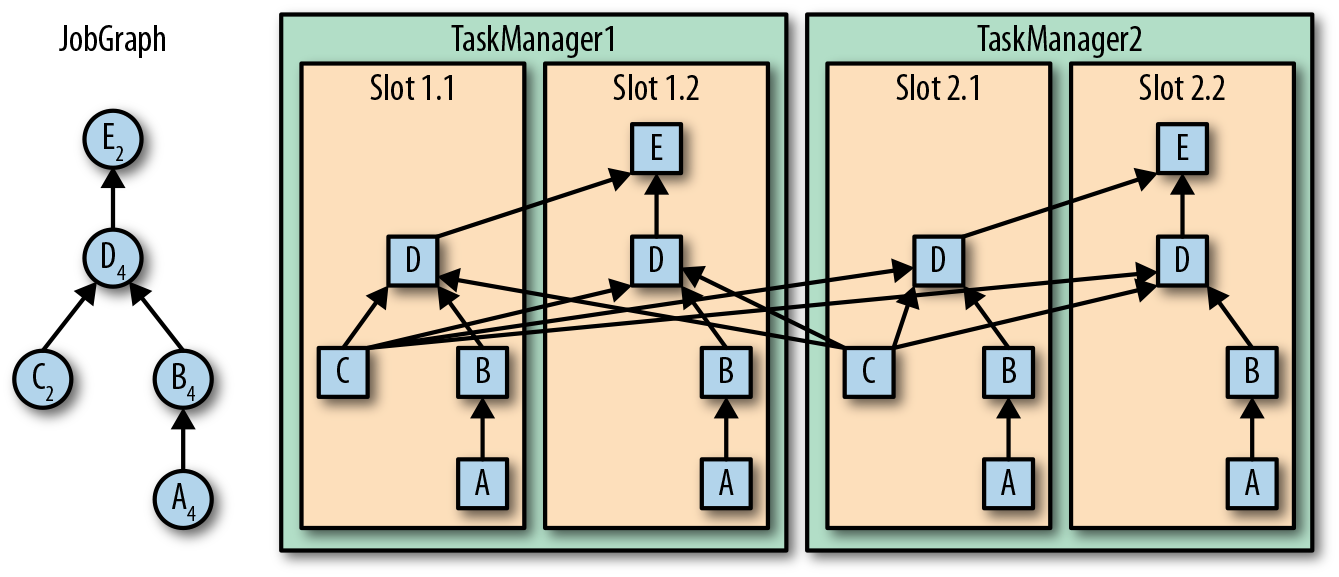
\includegraphics[width=0.7\textwidth]{images/spaf_0302.png}
    \caption{lambda架构}
\end{figure}

最左边是一个“作业图”（JobGraph），包含了5个算子——它是应用程序的非并行表示。其中算子A和C是数据源（source），E是输出端（sink）。C和E并行度为2，而其他的算子并行度为4。因为最高的并行度是4，所以应用需要至少四个slot来执行任务。现在有两个TaskManager，每个又各有两个slot，所以我们的需求是满足的。作业管理器将JobGraph转化为“执行图”（ExecutionGraph），并将任务分配到四个可用的slot上。对于有4个并行任务的算子，它的task会分配到每个slot上。而对于并行度为2的operator C和E，它们的任务被分配到slot 1.1、2.1 以及 slot 1.2、2.2。将tasks调度到slots上，可以让多个tasks跑在同一个TaskManager内，也就可以是的tasks之间的数据交换更高效。然而将太多任务调度到同一个TaskManager上会导致TaskManager过载，继而影响效率。之后我们会在“控制任务调度”一节继续讨论如何控制任务的调度。

TaskManager在同一个JVM中以多线程的方式执行任务。线程较进程会更轻量级，但是线程之间并没有对任务进行严格隔离。所以，单个任务的异常行为有可能会导致整个TaskManager进程挂掉，当然也同时包括运行在此进程上的所有任务。通过为每个TaskManager配置单独的slot，就可以将应用在TaskManager上相互隔离开来。TaskManager内部有多线程并行的机制，而且在一台主机上可以部署多个TaskManager，所以Flink在资源配置上非常灵活，在部署应用时可以充分权衡性能和资源的隔离。我们将会在第九章对Flink集群的配置和搭建继续做详细讨论。

\subsection{高可用配置}

流式应用程序一般被设计为7 x 24小时运行。所以很重要的一点是：即使出现了进程挂掉的情况，应用仍需要继续保持运行。为了从故障恢复，系统首先需要重启进程、然后重启应用并恢复它的状态。接下来，我们就来了解Flink如何重启失败的进程。

\textit{TaskManager故障}

如前所述，Flink需要足够数目的slot，来执行一个应用的所有任务。假设一个Flink环境有4个TaskManager，每个提供2个插槽，那么流应用程序执行的最高并行度为8。如果其中一个TaskManager挂掉了，那么可用的slots会降到6。在这种情况下，作业管理器会请求ResourceManager提供更多的slots。如果此请求无法满足——例如应用跑在一个独立集群——那么作业管理器在有足够的slots之前，无法重启应用。应用的重启策略决定了作业管理器的重启频率，以及两次重启尝试之间的时间间隔。

\textit{作业管理器故障}

比TaskManager故障更严重的问题是作业管理器故障。作业管理器控制整个流应用程序的执行，并维护执行中的元数据——例如指向已完成检查点的指针。若是对应的作业管理器挂掉，则流程序无法继续运行。所以这就导致在Flink应用中，作业管理器是单点故障。为了解决这个问题，Flink提供了高可用模式。在原先的作业管理器挂掉后，可以将一个作业的状态和元数据迁移到另一个作业管理器，并继续执行。

Flink的高可用模式基于Apache ZooKeeper，我们知道，ZooKeeper是用来管理需要协调和共识的分布式服务的系统。Flink主要利用ZooKeeper来进行领导者（leader）的选举，并把它作为一个高可用和持久化的数据存储。当在高可用模式下运行时，作业管理器会将JobGraph以及所有需要的元数据（例如应用程序的jar文件），写入到一个远程的持久化存储系统中。而且，作业管理器会将指向存储位置的指针，写入到ZooKeeper的数据存储中。在执行一个应用的过程中，作业管理器会接收每个独立任务检查点的状态句柄（也就是存储位置）。当一个检查点完成时（所有任务已经成功地将它们的状态写入到远程存储）， 作业管理器把状态句柄写入远程存储，并将指向这个远程存储的指针写入ZooKeeper。这样，一个作业管理器挂掉之后再恢复，所需要的所有数据信息已经都保存在了远程存储，而ZooKeeper里存有指向此存储位置的指针。图3-3描述了这个设计：

\begin{figure}[htbp]
    \centering
    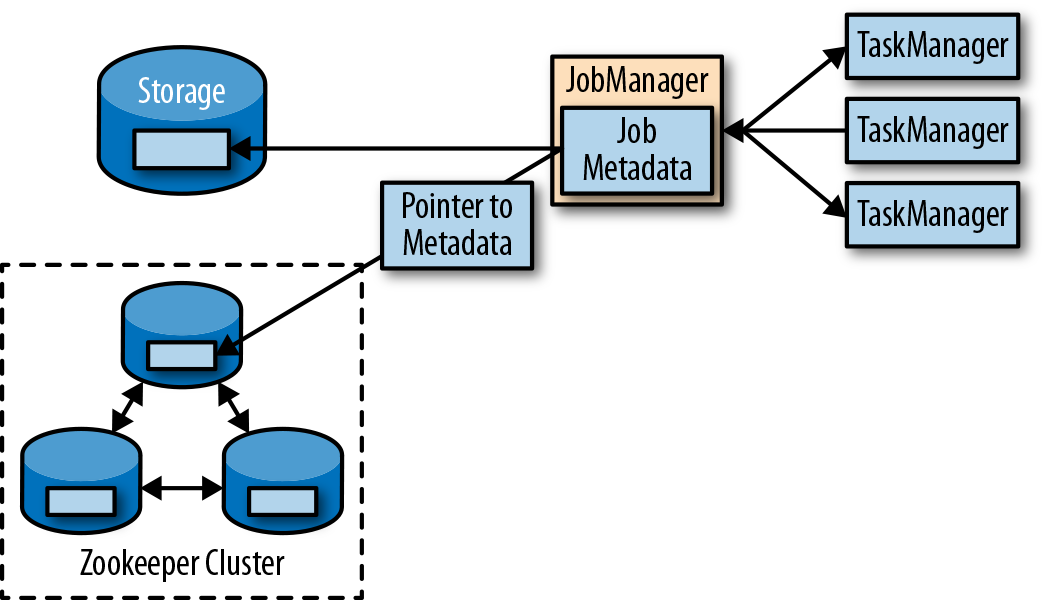
\includegraphics[width=0.7\textwidth]{images/spaf_0303.png}
    \caption{lambda架构}
\end{figure}

当一个作业管理器失败，所有属于这个应用的任务都会自动取消。一个新的作业管理器接管工作，会执行以下操作：

\begin{itemize}
    \item 从ZooKeeper请求存储位置（storage location），从远端存储获取JobGraph，Jar文件，以及应用最近一次检查点（checkpoint）的状态句柄（state handles）
    \item 从ResourceManager请求slots，用来继续运行应用
    \item 重启应用，并将所有任务的状态，重设为最近一次已完成的检查点
\end{itemize}

如果我们是在容器环境里运行应用（如Kubernetes），故障的作业管理器或TaskManager 容器通常会由容器服务自动重启。当运行在YARN或Mesos之上时，作业管理器或TaskManager进程会由Flink的保留进程自动触发重启。而在standalone模式下，Flink并未提供重启故障进程的工具。所以，此模式下我们可以增加备用（standby）的 作业管理器和TaskManager，用于接管故障的进程。我们将会在“高可用配置”一节中做进一步讨论。

\section{Flink中的数据传输}

\subsection{基于信任度的流控制}

通过网络连接来发送每条数据的效率很低，会导致很大的开销。为了充分利用网络连接的带宽，就需要进行缓冲了。在流处理的上下文中，缓冲的一个缺点是会增加延迟，因为数据需要在缓冲区中进行收集，而不是立即发送。

Flink实现了一个基于信任度的流量控制机制，其工作原理如下。接收任务授予发送任务一些“信任度”（credit），也就是为了接收其数据而保留的网络缓冲区数。当发送者收到一个信任度通知，它就会按照被授予的信任度，发送尽可能多的缓冲数据，并且同时发送目前积压数据的大小——也就是已填满并准备发送的网络缓冲的数量。接收者用保留的缓冲区处理发来的数据，并对发送者传来的积压量进行综合考量，为其所有连接的发送者确定下一个信用度授权的优先级。

基于信用度的流控制可以减少延迟，因为发送者可以在接收者有足够的资源接受数据时立即发送数据。此外，在数据倾斜的情况下，这样分配网络资源是一种很有效的机制，因为信用度是根据发送者积压数据量的规模授予的。因此，基于信用的流量控制是Flink实现高吞吐量和低延迟的重要组成部分。

\subsection{任务链}

Flink采用了一种称为任务链的优化技术，可以在特定条件下减少本地通信的开销。为了满足任务链的要求，必须将两个或多个算子设为相同的并行度，并通过本地转发（local forward）的方式进行连接。图3-5所示的算子管道满足这些要求。它由三个算子组成，这些算子的任务并行度都被设为2，并且通过本地转发方式相连接。

\begin{figure}[htbp]
    \centering
    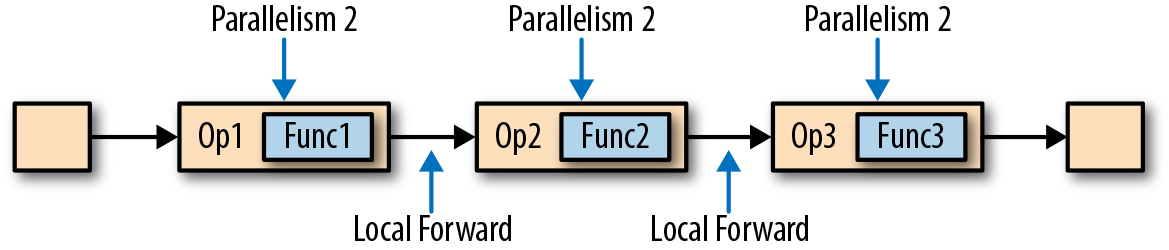
\includegraphics[width=0.7\textwidth]{images/spaf_0305.png}
    \caption{lambda架构}
\end{figure}

图3-6展示了管道以任务链方式运行的过程。算子的函数被融合成了一个单一的任务，由一个线程执行。由函数生成的数据通过一个简单的方法调用移交给下一个函数；这样在函数之间直接传递数据，基本上没有序列化和通信成本。

\begin{figure}[htbp]
    \centering
    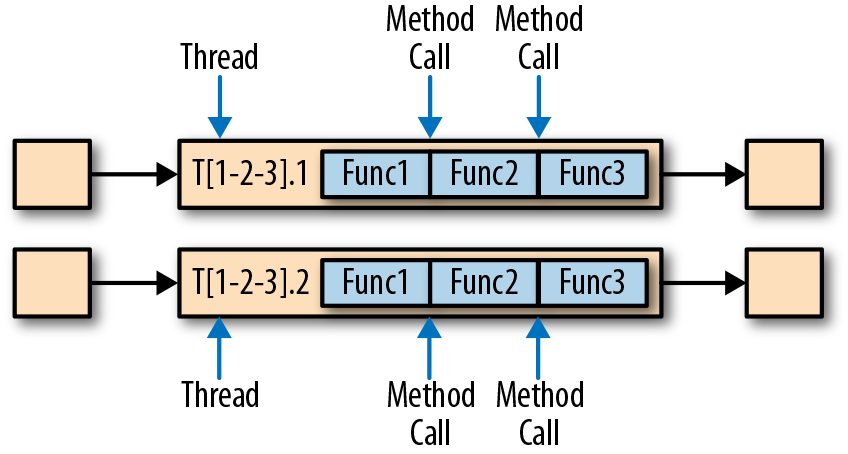
\includegraphics[width=0.7\textwidth]{images/spaf_0306.png}
    \caption{lambda架构}
\end{figure}

任务链可以显著降低本地任务之间的通信成本，但也有一些场景，在没有链接的情况下运行管道操作是有意义的。例如，如果任务链中某个函数执行的开销巨大，那就可以将一条长的任务链管道断开，或者将一条链断开为两个任务，从而可以将这个开销大的函数调度到不同的槽（slots）中。图3-7显示了在没有任务链的情况下相同管道操作的执行情况。所有函数都由独立的单个任务来评估，每个任务都在专有的线程中运行。

\begin{figure}[htbp]
    \centering
    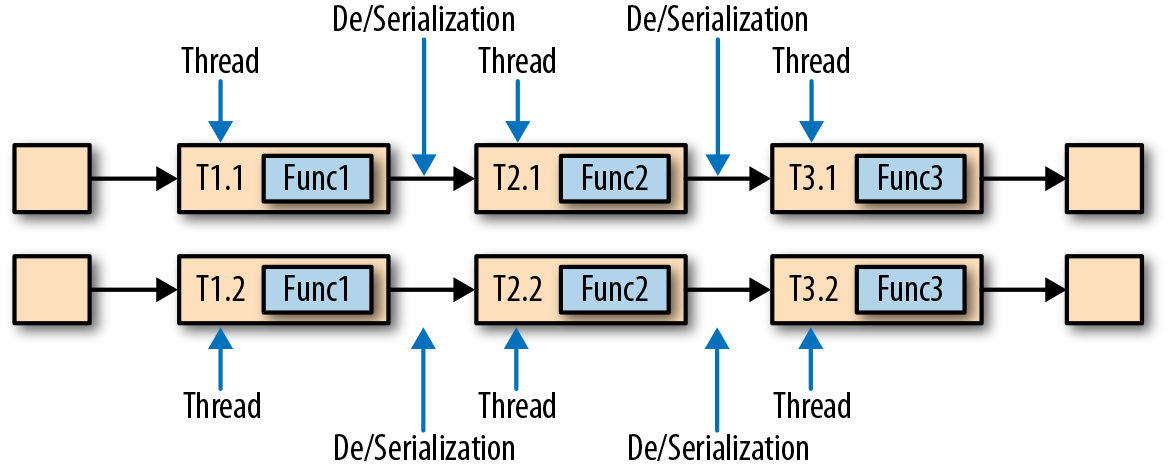
\includegraphics[width=0.7\textwidth]{images/spaf_0307.png}
    \caption{lambda架构}
\end{figure}

任务链在Flink中默认会启用。在“控制任务链”一节中，我们展示了如何禁用应用程序的任务链，以及如何控制各个算子的链接行为。

\section{事件时间处理}

在“时间语义”一节，我们重点强调了时间语义在流处理应用中的重要性，并且解释了处理时间（processing time）和事件时间（event time）的不同。处理时间比较好理解，因为它是基于处理器本地时间的；但同时，它会带来比较混乱、不一致、并且不可重现的结果。相比之下，事件时间语义能够产生可重现且一致的结果，这也是许多流处理场景希望解决的一大难题。但是，与处理时间应用程序相比，事件时间应用程序会更复杂，需要额外的配置。另外，支持事件时间的流处理器，也比纯粹在处理时间中运行的系统内部更为复杂。

Flink为常见的事件时间处理操作提供了直观且易于使用的原语，同时暴露了表达性很强的API，用户可以使用自定义算子实现更高级的事件时间应用程序。很好地理解Flink的内部时间处理，对于实现这样的高级应用程序会有很大帮助，有时也是必需的。上一章介绍了Flink利用两个概念来支持事件时间语义：记录时间戳（timestamps）和水位线（watermarks）。接下来，我们将描述Flink如何在内部实现并处理时间戳和水位线，进而支持具有事件时间语义的流式应用程序。

\subsection{时间戳}

由Flink事件时间流应用程序处理的所有记录都必须伴有时间戳。时间戳将数据与特定时间点相关联，通常就是数据所表示的事件发生的时间点。而只要时间戳大致跟数据流保持一致，基本上随着数据流的前进而增大，应用程序就可以自由选择时间戳的含义。不过正如“时间语义”一节中所讨论的，在现实场景中，时间戳基本上都是乱序的，所以采用“事件时间”而非“处理事件”往往会显得更为重要。

当Flink以事件时间模式处理数据流时，它会根据数据记录的时间戳来处理基于时间的算子。例如，时间窗口算子根据相关时间戳将数据分配给不同的时间窗口。Flink将时间戳编码为16字节的长整型值，并将其作为元数据附加到数据记录中。它的内置运算符会将这个长整型值解释为一个具有毫秒精度的Unix时间戳，也就是1970-01-01-00:00:00.000以来的毫秒数。当然，如果用户进行了自定义，那么运算符可以有自己的解释，例如，可以将精度调整到微秒。

\subsection{水位线}

除了时间戳，基于事件时间的Flink应用程序还必须支持水位线（watermark）。在基于事件时间的应用中，水位线用于生成每个任务的当前事件时间。基于时间的算子使用这个“当前事件时间”来触发计算和处理操作。例如，一个时间窗口任务（time-window task）会在任务的事件时间超出窗口的关闭边界时，完成窗口计算，并输出计算结果。

在Flink中，水位线被实现为一条特殊的数据记录，它里面以长整型值保存了一个时间戳。水位线在带有时间戳的数据流中，跟随着其它数据一起流动，如图3-8所示。

\begin{figure}[htbp]
    \centering
    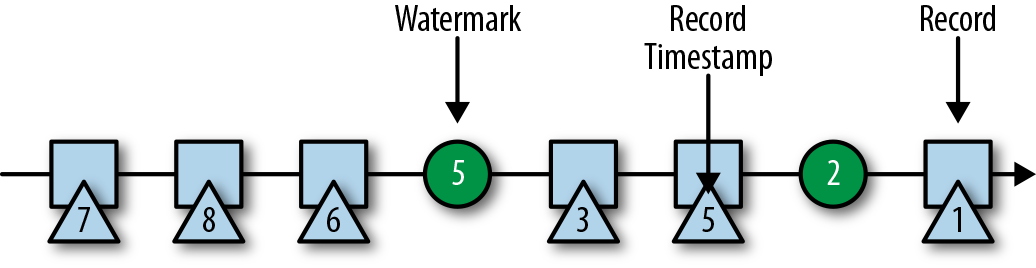
\includegraphics[width=0.7\textwidth]{images/spaf_0308.png}
    \caption{lambda架构}
\end{figure}

水位线有两个基本属性：

\begin{itemize}
    \item 必须单调递增，以确保任务的事件时间时钟在向前推进，而不是在后退。
    \item 它们与数据的时间戳相关。带有时间戳T的水位线表示，所有后续数据的时间戳都应该大于T。
\end{itemize}

上面的第二个属性用于处理带有乱序时间戳的数据流，比如图3-8中时间戳3和5的数据。基于时间的算子任务会收集和处理数据（这些数据可能具有乱序的时间戳），并在事件时间时钟到达某个时刻时完成计算。这个时刻就表示数据收集的截止，具有之前时间戳的数据应该都已经到达、不再需要了；而其中的事件时间时钟，正是由当前接收到的水位线来指示的。如果任务再接收到的数据违反了watermark的这一属性，也就是时间戳小于以前接收到的水位线时，它所属的那部分计算可能已经完成了。这种数据被称为延迟数据（late records）。Flink提供了处理延迟数据的不同方式，我们会在“处理延迟数据”一节中讨论。

水位线还有一个很有趣的特性，它允许应用程序自己来平衡结果的完整性和延迟。如果水位线与数据的时间戳非常接近，那么我们可以得到较低的处理延迟，因为任务在完成计算之前只会短暂地等待更多数据到达。而同时，结果的完整性可能会受到影响，因为相关数据可能因为迟到而被视为“延迟数据”，这样就不会包含在结果中。相反，非常保守的水位线提供了足够的时间去等待所有数据到达，这样会增加处理延迟，但提高了结果的完整性。

\subsection{watermark的传递和事件时间}

在本节中，我们将讨论算子如何处理水位线。Flink把watermark作为一条特殊的数据来实现，它也会由算子任务接收和发送。任务会有一个内部的时间服务，它会维护定时器，并在收到watermark时触发。任务可以在计时器服务中注册定时器，以便在将来特定的时间点执行计算。例如，窗口算子为每个活动窗口注册一个定时器，当事件时间超过窗口的结束时间时，该计时器将清除窗口的状态。

当任务收到watermark时，将执行以下操作：

\begin{itemize}
    \item 任务根据watermark的时间戳更新其内部事件时钟。
    \item 任务的时间服务会将所有过期的计时器标识出来，它们的时间小于当前的事件时间。对于每个过期的计时器，任务调用一个回调函数，该函数可以执行计算并发送结果。
    \item 任务会发出一个带有更新后的事件时间的watermark。
\end{itemize}

\begin{note}
    Flink限制通过DataStream API访问时间戳和watermark。函数不能读取或修改数据的时间戳和watermark，但底层的“处理函数”（process functions）除外，它们可以读取当前处理数据的时间戳、请求算子的当前事件时间，还可以注册定时器。通常的函数都不会暴露这些可以设置时间戳、操作任务事件时间时钟、或者发出水位线的API。而基于时间的数据流算子任务则会配置发送出的数据的时间戳，以确保它们能够与已到达的水位线平齐。例如，窗口计算完成后，时间窗口的算子任务会将窗口的结束时间作为时间戳附加到将要发送出的结果数据上，然后再使用触发窗口计算的时间戳发出watermark。
\end{note}

现在，让我们更详细地解释一下任务在接收到新的watermark时，如何继续发送watermark并更新其事件时钟。正如我们在“数据并发和任务并发”中所了解的，Flink将数据流拆分为多个分区，并通过单独的算子任务并行地处理每个分区。每个分区都是一个流，里面包含了带着时间戳的数据和watermark。一个算子与它前置或后续算子的连接方式有多种情况，所以它对应的任务可以从一个或多个“输入分区”接收数据和watermark，同时也可以将数据和watermark发送到一个或多个“输出分区”。接下来，我们将详细描述一个任务如何向多个输出任务发送watermark，以及如何通过接收到的watermark来驱动事件时间时钟前进。

任务为每个输入分区维护一个分区水位线（watermark）。当从一个分区接收到watermark时，它会比较新接收到的值和当前水位值，然后将相应的分区watermark更新为两者的最大值。然后，任务会比较所有分区watermark的大小，将其事件时钟更新为所有分区watermark的最小值。如果事件时间时钟前进了，任务就将处理所有被触发的定时器操作，并向所有连接的输出分区发送出相应的watermark，最终将新的事件时间广播给所有下游任务。

图3-9显示了具有四个输入分区和三个输出分区的任务如何接收watermark、更新分区watermark和事件时间时钟，以及向下游发出watermark。

\begin{figure}[htbp]
    \centering
    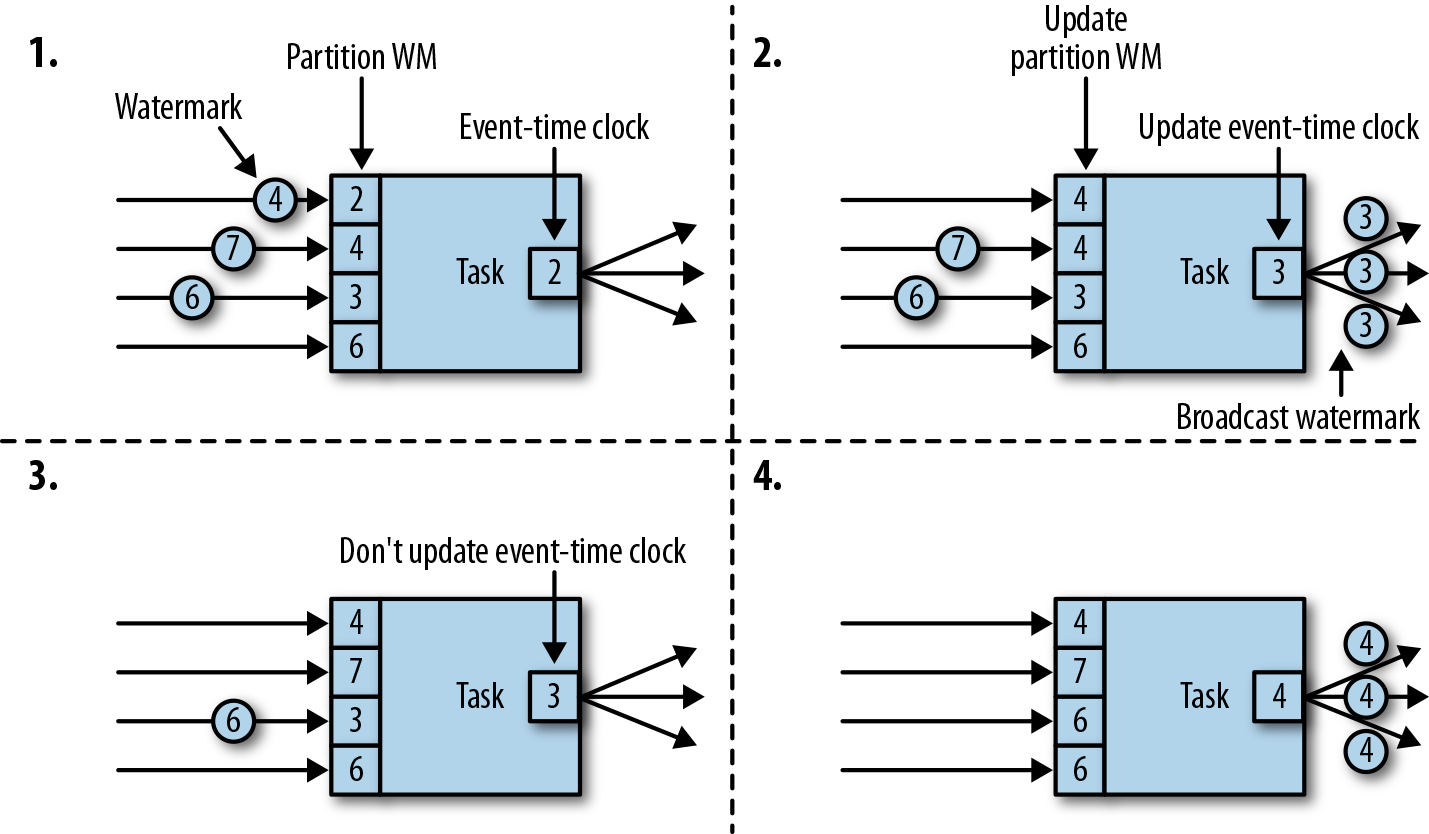
\includegraphics[width=0.7\textwidth]{images/spaf_0309.png}
    \caption{lambda架构}
\end{figure}

具有两个或多个输入流（如Union或CoFlatMap）的算子任务（参见“多流转换”一节）也会以所有分区watermark的最小值作为事件时间时钟。它们并不区分不同输入流的分区watermark，所以两个输入流的数据都是基于相同的事件时间时钟进行处理的。当然我们可以想到，如果应用程序的各个输入流的事件时间不一致，那么这种处理方式可能会导致问题。

Flink的水位处理和传递算法，确保了算子任务发出的时间戳和watermark是“对齐”的。不过它依赖一个条件，那就是所有分区都会提供不断增长的watermark。一旦一个分区不再推进水位线的上升，或者完全处于空闲状态、不再发送任何数据和watermark，任务的事件时间时钟就将停滞不前，任务的定时器也就无法触发了。对于基于时间的算子来说，它们需要依赖时钟的推进来执行计算和清除状态，这种情况显然就会有问题。如果任务没有定期从所有输入任务接收到新的watermark，那么基于时间的算子的处理延迟和状态空间的大小都会显著增加。

对于具有两个输入流而且watermark明显不同的算子，也会出现类似的情况。具有两个输入流的任务的事件时间时钟，将会同较慢的那条流的watermark保持一致，而通常较快流的数据或者中间结果会在state中缓冲，直到事件时间时钟达到这条流的watermark，才会允许处理它们。

\subsection{时间戳的分配和水位线的产生}

我们已经解释了什么是时间戳和水位线，以及它们是如何由Flink内部处理的；然而我们还没有讨论它们的产生。流应用程序接收到数据流时，通常就会先分配时间戳并生成水位线（watermark）。因为时间戳的选择是由不同的应用程序决定的，而且watermark取决于时间戳和流的特性，所以应用程序必须首先显式地分配时间戳并生成watermark。Flink流应用程序可以通过三种方式分配时间戳和生成watermark：

\begin{itemize}
    \item 在数据源（source）处分配：当数据流被摄入到应用程序中时，可以由“源函数”SourceFunction分配和生成时间戳和watermark。SourceFunction可以产生并发送一个数据流；数据会与相关的时间戳一起发送出去，而watermark可以作为一条特殊数据在任何时间点发出。如果SourceFunction（暂时）不再发出watermark，它可以声明自己处于“空闲”（idle）状态。Flink会在后续算子的水位计算中，把空闲的SourceFunction产生的流分区排除掉。source的这一空闲机制，可以用来解决前面提到的水位不再上升的问题。源函数（Source Function）在“实现自定义源函数”一节中进行了更详细的讨论。
    \item 定期分配：在Flink中，DataStream API提供一个名为AssignerWithPeriodicWatermarks的用户定义函数，它可以从每个数据中提取时间戳，并被定期调用以生成当前watermark。提取出的时间戳被分配给相应的数据，而生成的watermark也会添加到流中。这个函数将在“分配时间戳和生成水位线”一节中讨论。
    \item 间断分配：AssignerWithPunctuatedWatermarks是另一个用户定义的函数，它同样会从每个数据中提取一个时间戳。它可以用于生成特殊输入数据中的watermark。与AssignerWithPeriodicWatermarks相比，此函数可以（但不是必须）从每个记录中提取watermark。我们在“分配时间戳和生成水位线”一节中同样讨论了该函数。
\end{itemize}

用户定义的时间戳分配函数并没有严格的限制，通常会放在尽可能靠近source算子的位置，因为当经过一些算子处理后，数据及其时间戳的顺序就更加难以解释了。所以尽管我们可以在流应用程序的中段覆盖已有的时间戳和watermark——Flink通过用户定义的函数提供了这种灵活性，但这显然并不是推荐的做法。

\section{状态管理}

在第2章中，我们已经知道大多数流应用程序都是有状态的。许多算子会不断地读取和更新状态，例如在窗口中收集的数据、读取输入源的位置，或者像机器学习模型那样的用户定制化的算子状态。 Flink用同样的方式处理所有的状态，无论是内置的还是用户自定义的算子。本节我们将会讨论Flink支持的不同类型的状态，并解释“状态后端”是如何存储和维护状态的。

一般来说，由一个任务维护，并且用来计算某个结果的所有数据，都属于这个任务的状态。你可以认为状态就是一个本地变量，可以被任务的业务逻辑访问。图3-10显示了任务与其状态之间的交互。

\begin{figure}[htbp]
    \centering
    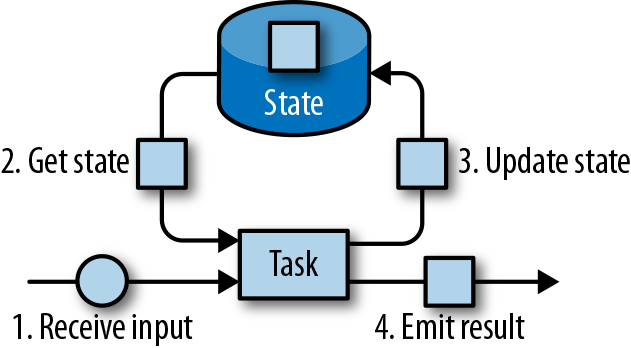
\includegraphics[width=0.7\textwidth]{images/spaf_0310.png}
    \caption{lambda架构}
\end{figure}

任务会接收一些输入数据。在处理数据时，任务可以读取和更新状态，并根据输入数据和状态计算结果。最简单的例子，就是统计接收到多少条数据的任务。当任务收到新数据时，它会访问状态以获取当前的计数，然后让计数递增，更新状态并发送出新的计数。

应用程序里，读取和写入状态的逻辑一般都很简单直接，而有效可靠的状态管理会复杂一些。这包括如何处理很大的状态——可能会超过内存，并且保证在发生故障时不会丢失任何状态。幸运的是，Flink会帮我们处理这相关的所有问题，包括状态一致性、故障处理以及高效存储和访问，以便开发人员可以专注于应用程序的逻辑。

在Flink中，状态始终与特定算子相关联。为了使运行时的Flink了解算子的状态，算子需要预先注册其状态。总的说来，有两种类型的状态：算子状态（operator state）和键控状态（keyed state），它们有着不同的范围访问，我们将在下面展开讨论。

\subsection{算子状态}

算子状态的作用范围限定为算子任务。这意味着由同一并行任务所处理的所有数据都可以访问到相同的状态，状态对于同一任务而言是共享的。算子状态不能由相同或不同算子的另一个任务访问。图3-11显示了任务如何访问算子状态。

\begin{figure}[htbp]
    \centering
    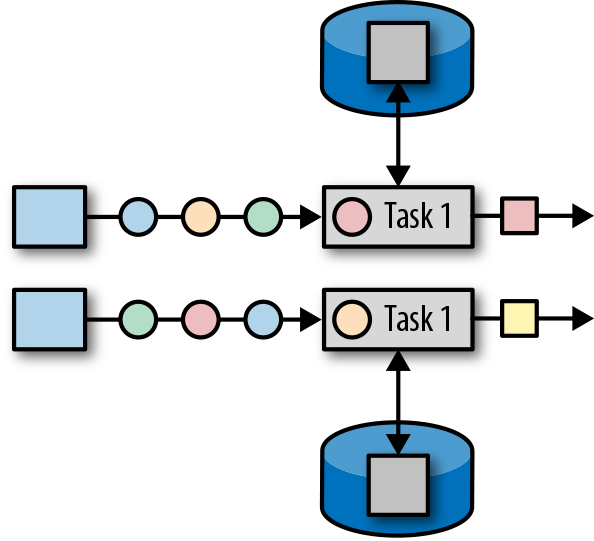
\includegraphics[width=0.7\textwidth]{images/spaf_0311.png}
    \caption{lambda架构}
\end{figure}

Flink为算子状态提供三种基本数据结构：

\begin{itemize}
    \item 列表状态：将状态表示为一组数据的列表。
    \item 联合列表状态：也将状态表示为数据的列表。它与常规列表状态的区别在于，在发生故障时，或者从保存点（savepoint）启动应用程序时如何恢复。我们将在后面继续讨论。
    \item 广播状态：如果一个算子有多项任务，而它的每项任务状态又都相同，那么这种特殊情况最适合应用广播状态。在保存检查点和重新调整算子并行度时，会用到这个特性。这两部分内容将在本章后面讨论。
\end{itemize}

\subsection{键控状态}

顾名思义，键控状态是根据输入数据流中定义的键（key）来维护和访问的。Flink为每个键值维护一个状态实例，并将具有相同键的所有数据，都分区到同一个算子任务中，这个任务会维护和处理这个key对应的状态。当任务处理一条数据时，它会自动将状态的访问范围限定为当前数据的key。因此，具有相同key的所有数据都会访问相同的状态。图3-12显示了任务如何与键控状态进行交互。

\begin{figure}[htbp]
    \centering
    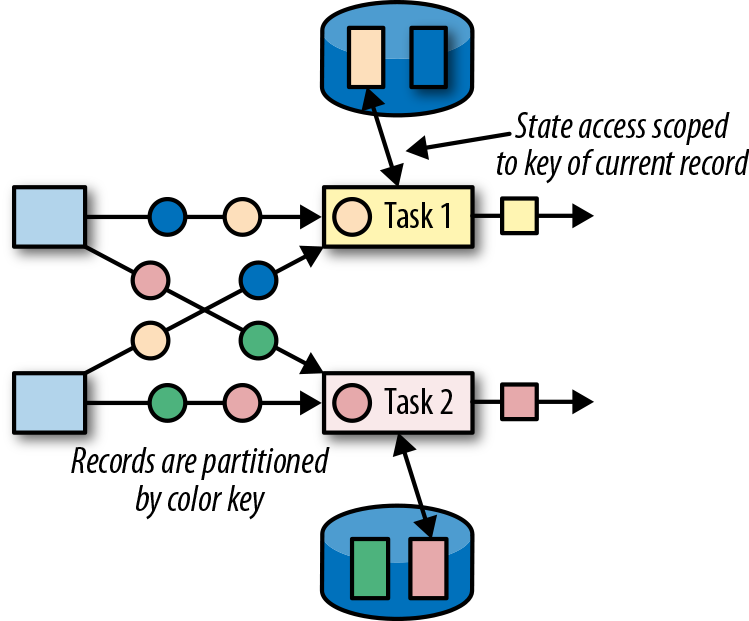
\includegraphics[width=0.7\textwidth]{images/spaf_0312.png}
    \caption{lambda架构}
\end{figure}

我们可以将键控状态看成是在算子所有并行任务上，对键进行分区（或分片）之后的一个键值映射（key-value map）。Flink为键控状态提供不同的数据结构，用于确定map中每个key存储的值的类型。我们简单了解一下最常见的键控状态。

\begin{itemize}
    \item 值状态：为每个键存储一个任意类型的单个值。复杂数据结构也可以存储为值状态。
    \item 列表状态：为每个键存储一个值的列表。列表里的每个数据可以是任意类型。
    \item 映射状态：为每个键存储一个键值映射（map）。map的key和value可以是任意类型。
\end{itemize}

状态的数据结构可以让Flink实现更有效的状态访问。我们将在“在运行时上下文（RuntimeContext）中声明键控状态”中做进一步讨论。

\subsection{状态后端}

每传入一条数据，有状态的算子任务都会读取和更新状态。由于有效的状态访问对于处理数据的低延迟至关重要，因此每个并行任务都会在本地维护其状态，以确保快速的状态访问。状态到底是如何被存储、访问以及维护的？这件事由一个可插入的组件决定，这个组件就叫做状态后端（state backend）。状态后端主要负责两件事：本地的状态管理，以及将检查点（checkpoint）状态写入远程存储。

对于本地状态管理，状态后端会存储所有键控状态，并确保所有的访问都被正确地限定在当前键范围。Flink提供了默认的状态后端，会将键控状态作为内存中的对象进行管理，将它们存储在JVM堆上。另一种状态后端则会把状态对象进行序列化，并将它们放入RocksDB中，然后写入本地硬盘。第一种方式可以提供非常快速的状态访问，但它受内存大小的限制；而访问RocksDB状态后端存储的状态速度会较慢，但其状态可以增长到非常大。

状态检查点的写入也非常重要，这是因为Flink是一个分布式系统，而状态只能在本地维护。TaskManager进程（所有任务在其上运行）可能在任何时间点挂掉。因此，它的本地存储只能被认为是不稳定的。状态后端负责将任务的状态检查点写入远程的持久存储。写入检查点的远程存储可以是分布式文件系统，也可以是数据库。不同的状态后端在状态检查点的写入机制方面有所不同。例如，RocksDB状态后端支持增量的检查点，这对于非常大的状态来说，可以显著减少状态检查点写入的开销。

我们将在“选择状态后端”一节中更详细地讨论不同的状态后端及其优缺点。

\subsection{调整有状态算子的并行度}

流应用程序的一个常见要求是，为了增大或较小输入数据的速率，需要灵活地调整算子的并行度。对于无状态算子而言，并行度的调整没有任何问题，但更改有状态算子的并行度显然就没那么简单了，因为它们的状态需要重新分区并分配给更多或更少的并行任务。
Flink支持四种模式来调整不同类型的状态。

具有键控状态的算子通过将键重新分区为更少或更多任务来缩放并行度。不过，并行度调整时任务之间会有一些必要的状态转移。为了提高效率，Flink并不会对单独的key做重新分配，而是用所谓的``键组''（key
group）把键管理起来。键组是key的分区形式，同时也是Flink为任务分配key的方式。图3-13显示了如何在键组中重新分配键控状态。

\begin{figure}[htbp]
    \centering
    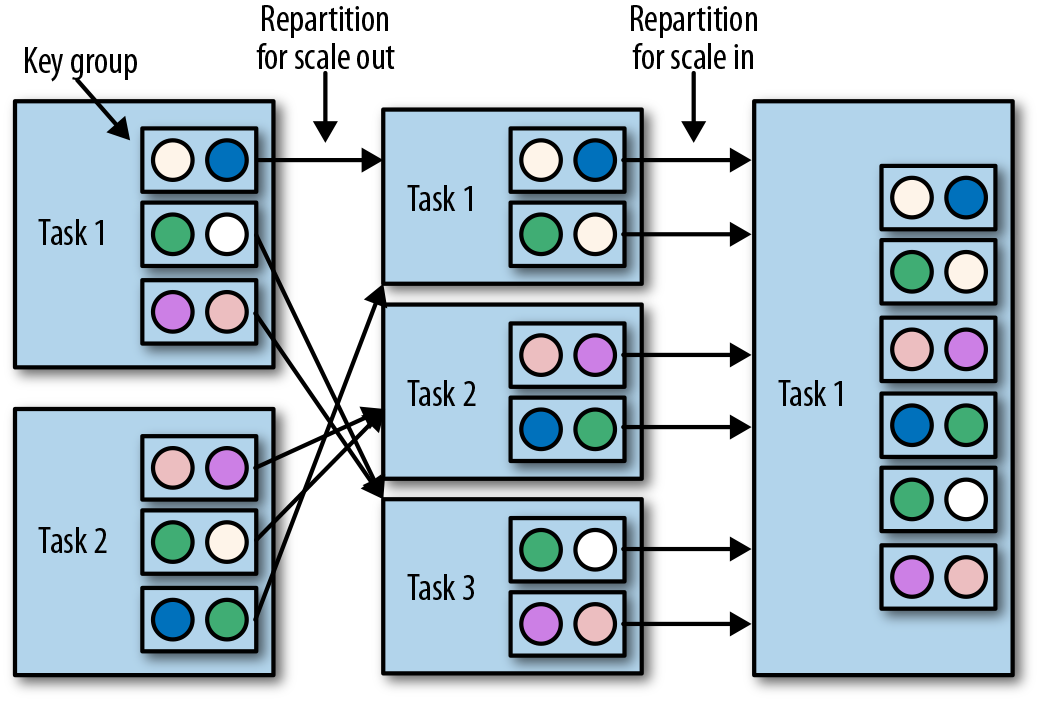
\includegraphics[width=0.7\textwidth]{images/spaf_0313.png}
    \caption{lambda架构}
\end{figure}

具有算子列表状态的算子，会通过重新分配列表中的数据项目来进行并行度缩放。从概念上讲，所有并行算子任务的列表项目会被收集起来，并将其均匀地重新分配给更少或更多的任务。如果列表条目少于算子的新并行度，则某些任务将以空状态开始。图3-14显示了算子列表状态的重新分配。

\begin{figure}[htbp]
    \centering
    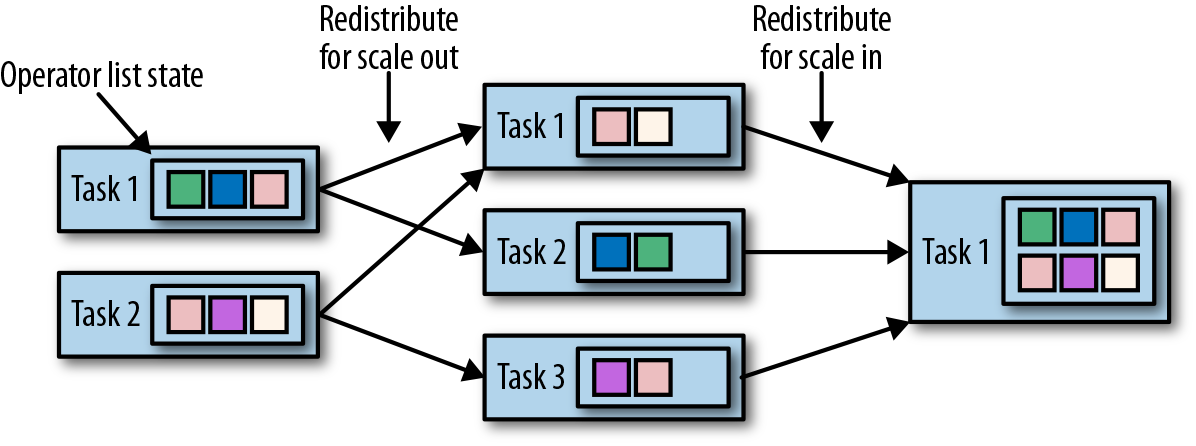
\includegraphics[width=0.7\textwidth]{images/spaf_0314.png}
    \caption{lambda架构}
\end{figure}

具有算子联合列表状态的算子，会通过向每个任务广播状态的完整列表，来进行并行度的缩放。然后，任务可以选择要使用的状态项和要丢弃的状态项。图3-15显示了如何重新分配算子联合列表状态。

\begin{figure}[htbp]
    \centering
    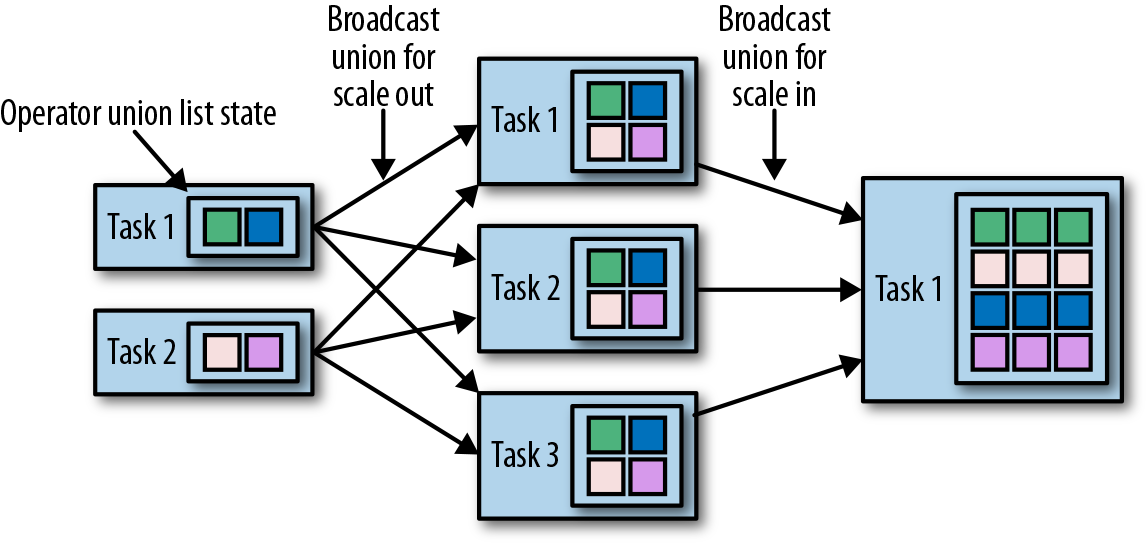
\includegraphics[width=0.7\textwidth]{images/spaf_0315.png}
    \caption{lambda架构}
\end{figure}

具有算子广播状态的算子，通过将状态复制到新任务，来增大任务的并行度。这是没问题的，因为广播状态保证了所有任务都具有相同的状态。而对于缩小并行度的情况，我们可以直接取消剩余任务，因为状态是相同的，已经被复制并且不会丢失。图3-16显示了算子广播状态的重新分配。

\begin{figure}[htbp]
    \centering
    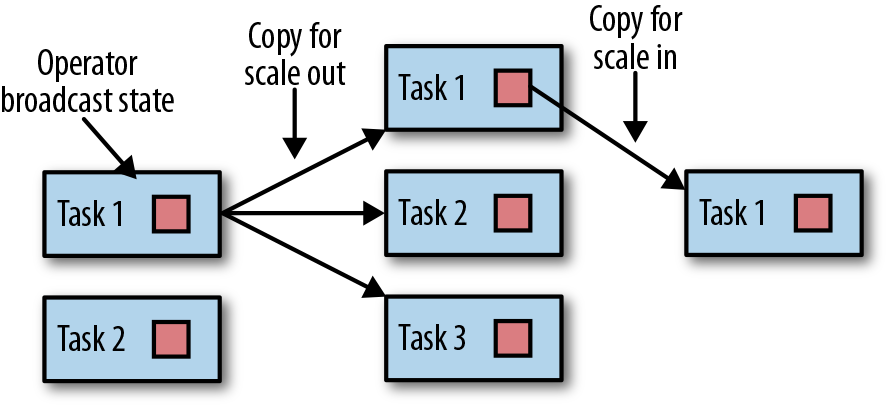
\includegraphics[width=0.7\textwidth]{images/spaf_0316.png}
    \caption{lambda架构}
\end{figure}

\section{检查点，保存点和状态恢复}

Flink是一个分布式数据处理系统，因此必须有一套机制处理各种故障，比如被杀掉的进程，故障的机器和中断的网络连接。任务都是在本地维护状态的，所以Flink必须确保状态不会丢失，并且在发生故障时能够保持一致。

在本节中，我们将介绍Flink的检查点（checkpoint）和恢复机制，这保证了“精确一次”（exactly-once）的状态一致性。我们还会讨论Flink独特的保存点（savepoint）功能，这是一个“瑞士军刀”式的工具，可以解决许多操作数据流时面对的问题。

\subsection{一致的检查点}

Flink的恢复机制的核心，就是应用状态的一致检查点。有状态流应用的一致检查点，其实就是所有任务状态在某个时间点的一份拷贝，而这个时间点应该是所有任务都恰好处理完一个相同的输入数据的时候。这个过程可以通过一致检查点的一个简单算法步骤来解释。这个算法的步骤是：

\begin{itemize}
\item 暂停所有输入流的摄取，也就是不再接收新数据的输入。
\item 等待所有正在处理的数据计算完毕，这意味着结束时，所有任务都已经处理了所有输入数据。
\item 通过将每个任务的状态复制到远程持久存储，来得到一个检查点。所有任务完成拷贝操作后，检查点就完成了。
\item 恢复所有输入流的摄取。
\end{itemize}

需要注意，Flink实现的并不是这种简单的机制。我们将在本节后面介绍Flink更精妙的检查点算法。

图3-17显示了一个简单应用中的一致检查点。

\begin{figure}[htbp]
    \centering
    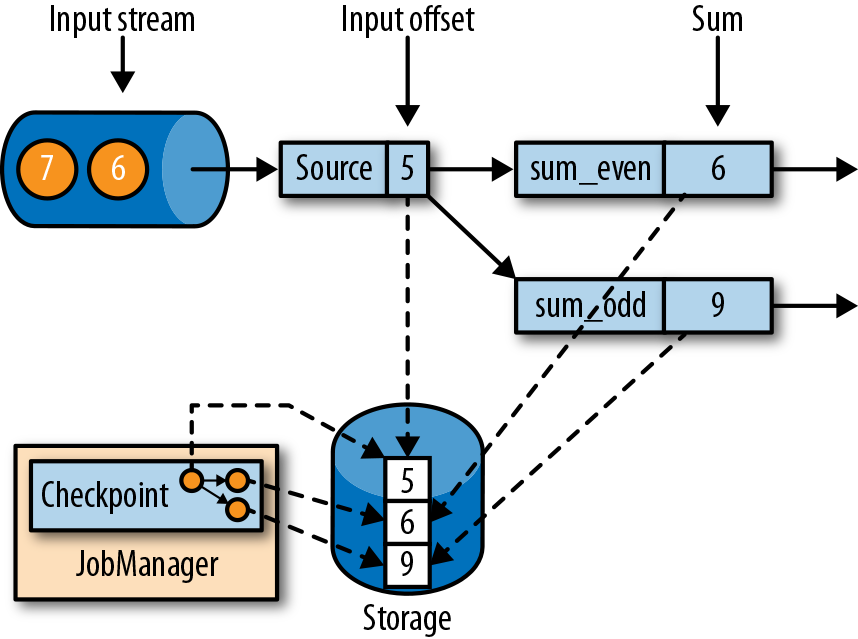
\includegraphics[width=0.7\textwidth]{images/spaf_0317.png}
    \caption{lambda架构}
\end{figure}

上面的应用程序中具有单一的输入源（source）任务，输入数据就是一组不断增长的数字的流------1,2,3等。数字流被划分为偶数流和奇数流。求和算子（sum）的两个任务会分别实时计算当前所有偶数和奇数的总和。源任务会将其输入流的当前偏移量存储为状态，而求和任务则将当前的总和值存储为状态。在图3-17中，Flink在输入偏移量为5时，将检查点写入了远程存储，当前的总和为6和9。

\subsection{从一致检查点中恢复状态}

在执行流应用程序期间，Flink会定期检查状态的一致检查点。如果发生故障，Flink将会使用最近的检查点来一致恢复应用程序的状态，并重新启动处理流程。图3-18显示了恢复过程。

\begin{figure}[htbp]
    \centering
    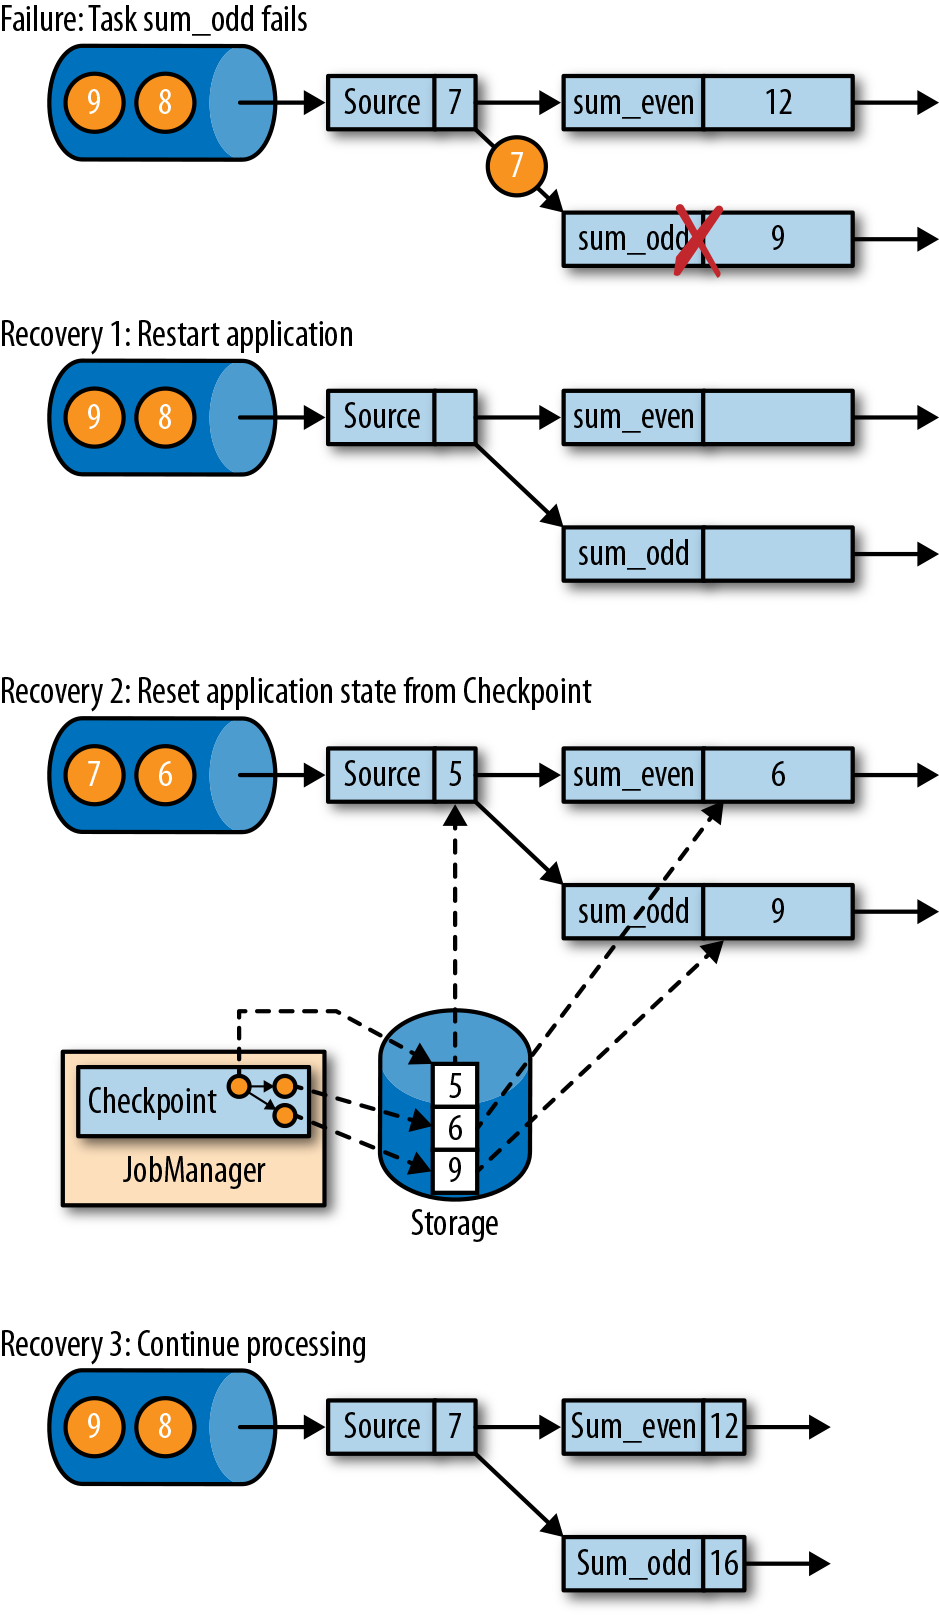
\includegraphics[width=0.7\textwidth]{images/spaf_0318.png}
    \caption{lambda架构}
\end{figure}

应用程序从检查点的恢复分为三步：

\begin{itemize}
\item 重新启动整个应用程序。
\item 将所有的有状态任务的状态重置为最近一次的检查点。
\item 恢复所有任务的处理。
\end{itemize}

这种检查点的保存和恢复机制可以为应用程序状态提供“精确一次”（exactly-once）的一致性，因为所有算子都会保存检查点并恢复其所有状态，这样一来所有的输入流就都会被重置到检查点完成时的位置。至于数据源是否可以重置它的输入流，这取决于其实现方式和消费流数据的外部接口。例如，像Apache Kafka这样的事件日志系统可以提供流上之前偏移位置的数据，所以我们可以将源重置到之前的偏移量，重新消费数据。而从套接字（socket）消费数据的流就不能被重置了，因为套接字的数据一旦被消费就会丢弃掉。因此，对于应用程序而言，只有当所有的输入流消费的都是可重置的数据源时，才能确保在“精确一次”的状态一致性下运行。

从检查点重新启动应用程序后，其内部状态与检查点完成时的状态完全相同。然后它就会开始消费并处理检查点和发生故障之间的所有数据。尽管这意味着Flink会对一些数据处理两次（在故障之前和之后），我们仍然可以说这个机制实现了精确一次的一致性语义，因为所有算子的状态都已被重置，而重置后的状态下还不曾看到这些数据。

我们必须指出，Flink的检查点保存和恢复机制仅仅可以重置流应用程序的内部状态。对于应用中的一些的输出（sink）算子，在恢复期间，某些结果数据可能会多次发送到下游系统，比如事件日志、文件系统或数据库。对于某些存储系统，Flink提供了具有精确一次输出功能的sink函数，比如，可以在检查点完成时提交发出的记录。另一种适用于许多存储系统的方法是幂等更新。在“应用程序一致性保证”一节中，我们还会详细讨论如何解决应用程序端到端的精确一次一致性问题。

\subsection{Flink的检查点算法}

Flink的恢复机制，基于它的一致性检查点。前面我们已经了解了从流应用中创建检查点的简单方法——先暂停应用，保存检查点，然后再恢复应用程序，这种方法很好理解，但它的理念是“停止一切”，这对于即使是中等延迟要求的应用程序而言也是不实用的。所以Flink没有这么简单粗暴，而是基于Chandy-Lamport算法实现了分布式快照的检查点保存。该算法并不会暂停整个应用程序，而是将检查点的保存与数据处理分离，这样就可以实现在其它任务做检查点状态保存状态时，让某些任务继续进行而不受影响。接下来我们将解释此算法的工作原理。

Flink的检查点算法用到了一种称为“检查点分界线”（checkpoint barrier）的特殊数据形式。与水位线（watermark）类似，检查点分界线由source算子注入到常规的数据流中，它的位置是限定好的，不能超过其他数据，也不能被后面的数据超过。检查点分界线带有检查点ID，用来标识它所属的检查点；这样，这个分界线就将一条流逻辑上分成了两部分。分界线之前到来的数据导致的状态更改，都会被包含在当前分界线所属的检查点中；而基于分界线之后的数据导致的所有更改，就会被包含在之后的检查点中。

我们用一个简单的流应用程序作为示例，来一步一步解释这个算法。该应用程序有两个源（source）任务，每个任务都消费一个增长的数字流。源任务的输出被划分为两部分：偶数和奇数的流。每个分区由一个任务处理，该任务计算所有收到的数字的总和，并将更新的总和转发给输出（sink）任务。这个应用程序的结构如图3-19所示。

\begin{figure}[htbp]
    \centering
    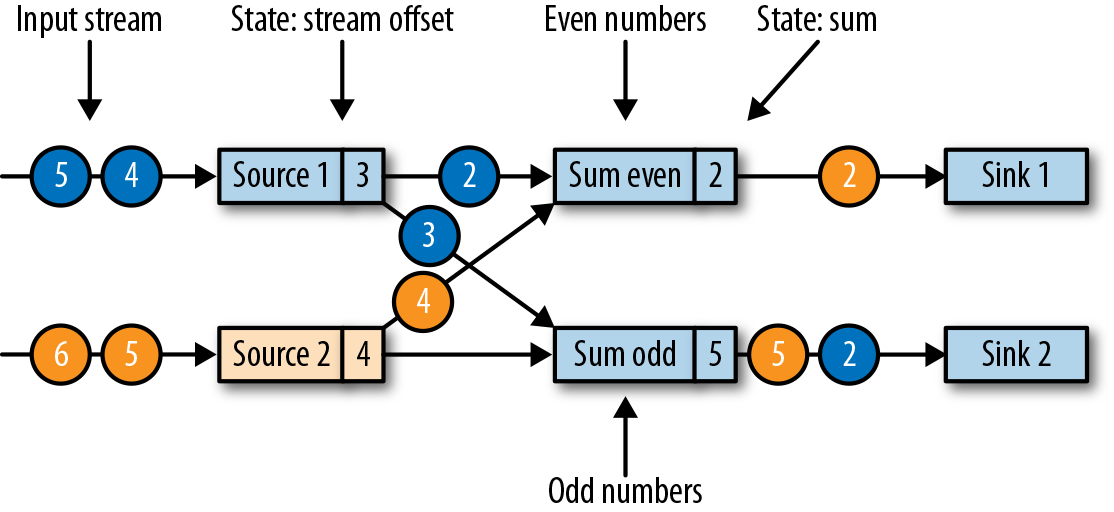
\includegraphics[width=0.7\textwidth]{images/spaf_0319.png}
    \caption{lambda架构}
\end{figure}

作业管理器会向每个数据源（source）任务发送一条带有新检查点ID的消息，通过这种方式来启动检查点，如图3-20所示。

\begin{figure}[htbp]
    \centering
    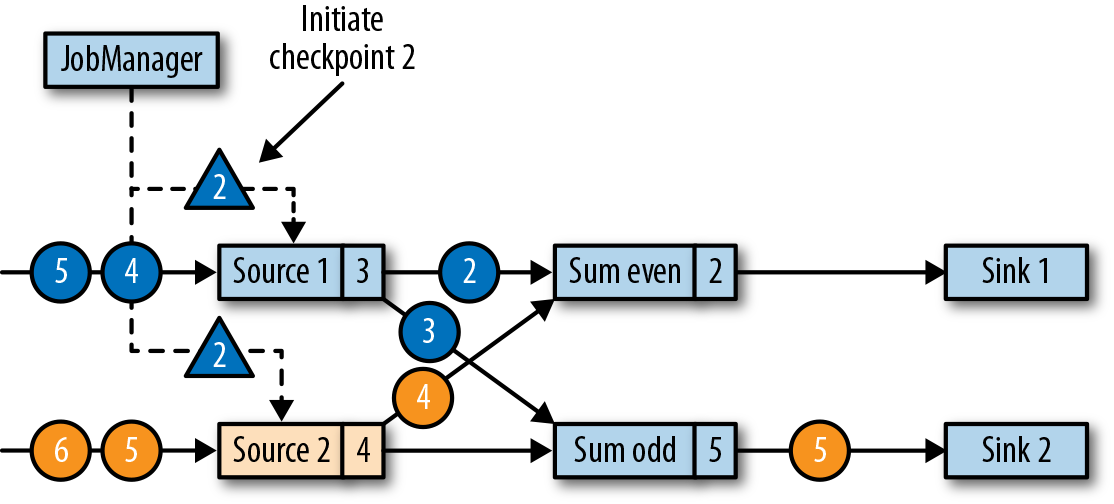
\includegraphics[width=0.7\textwidth]{images/spaf_0320.png}
    \caption{lambda架构}
\end{figure}

当source任务收到消息时，它会暂停发出新的数据，在状态后端触发本地状态的检查点保存，并向所有传出的流分区广播带着检查点ID的分界线（barriers）。状态后端在状态检查点完成后会通知任务，而任务会向作业管理器确认检查点完成。在发出所有分界线后，source任务就可以继续常规操作，发出新的数据了。通过将分界线注入到输出流中，源函数（source
function）定义了检查点在流中所处的位置。图3-21显示了两个源任务将本地状态保存到检查点，并发出检查点分界线之后的流应用程序。

\begin{figure}[htbp]
    \centering
    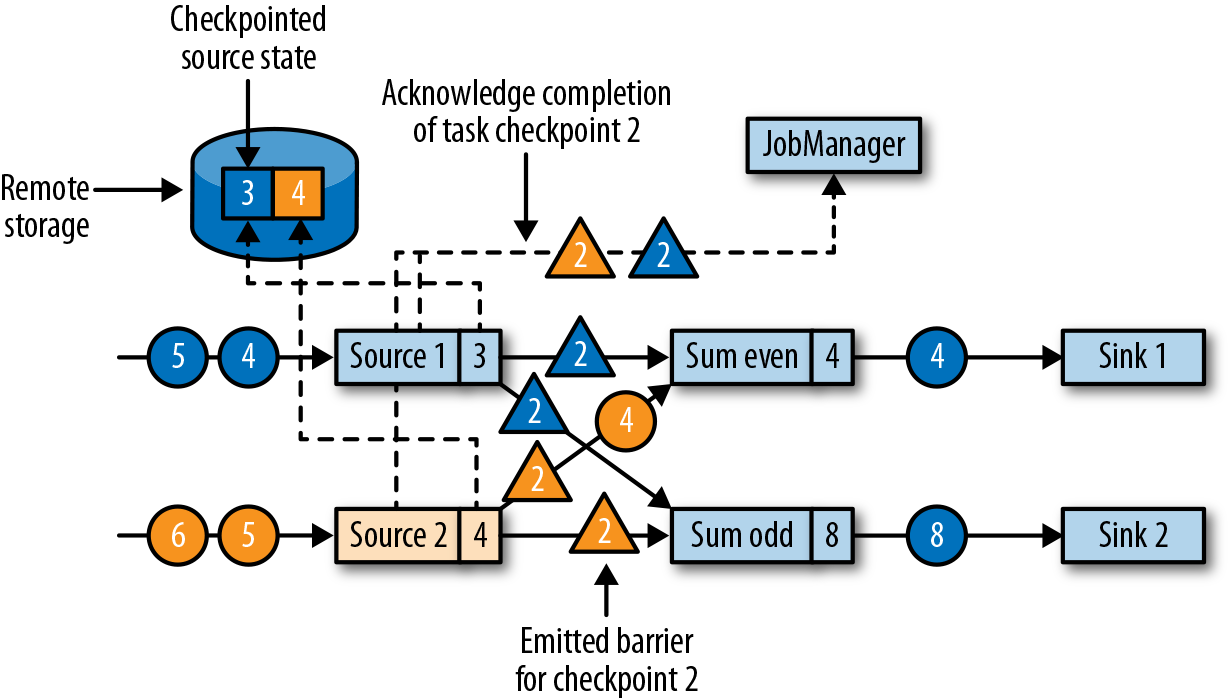
\includegraphics[width=0.7\textwidth]{images/spaf_0321.png}
    \caption{lambda架构}
\end{figure}

源任务发出的检查点分界线（barrier），将被传递给所连接的任务。与水位线（watermark）类似，barrier会被广播到所有连接的并行任务，以确保每个任务从它的每个输入流中都能接收到。当任务收到一个新检查点的barrier时，它会等待这个检查点的所有输入分区的barrier到达。在等待的过程中，任务并不会闲着，而是会继续处理尚未提供barrier的流分区中的数据。对于那些barrier已经到达的分区，如果继续有新的数据到达，它们就不会被立即处理，而是先缓存起来。这个等待所有分界线到达的过程，称为``分界线对齐''（barrier
alignment），如图3-22所示。

\begin{figure}[htbp]
    \centering
    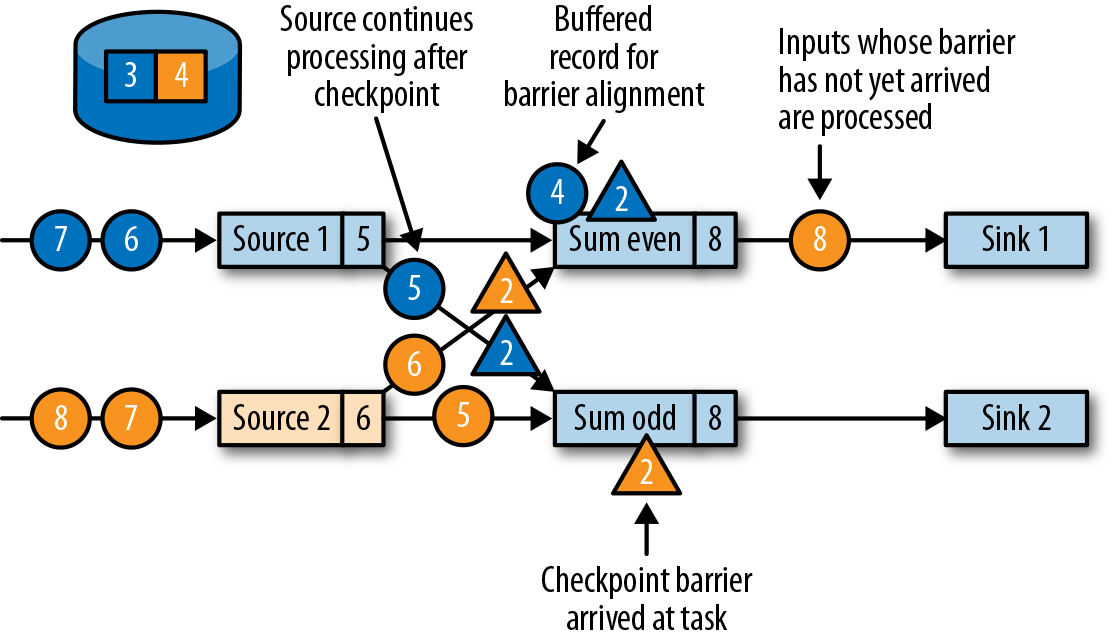
\includegraphics[width=0.7\textwidth]{images/spaf_0322.png}
    \caption{lambda架构}
\end{figure}

当任务从所有输入分区都收到barrier时，它就会在状态后端启动一个检查点的保存，并继续向所有下游连接的任务广播检查点分界线，如图3-23所示。

\begin{figure}[htbp]
    \centering
    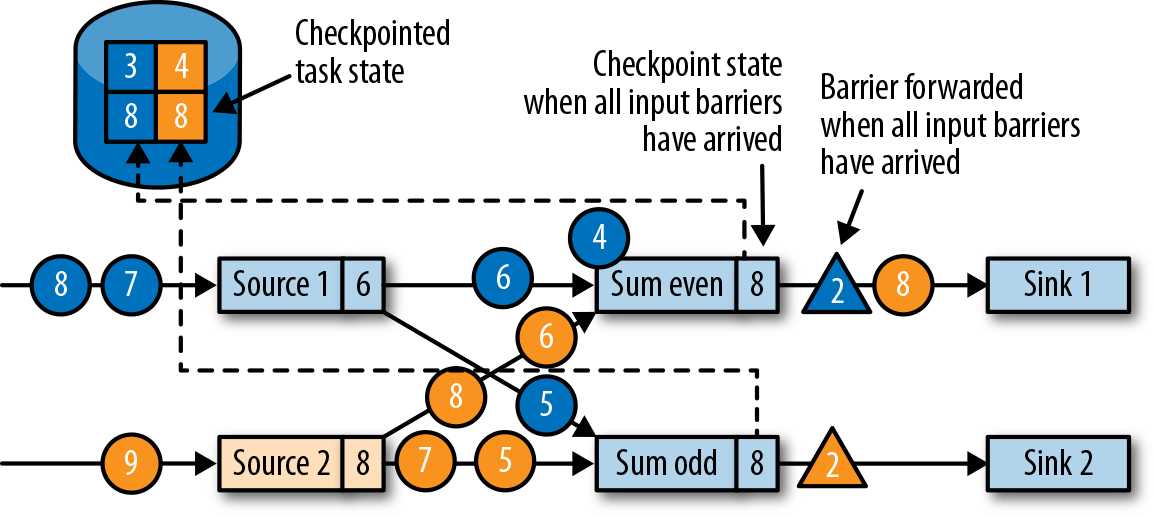
\includegraphics[width=0.7\textwidth]{images/spaf_0323.png}
    \caption{lambda架构}
\end{figure}

所有的检查点barrier都发出后，任务就开始处理之前缓冲的数据。在处理并发出所有缓冲数据之后，任务就可以继续正常处理输入流了。图3-24显示了此时的应用程序。

\begin{figure}[htbp]
    \centering
    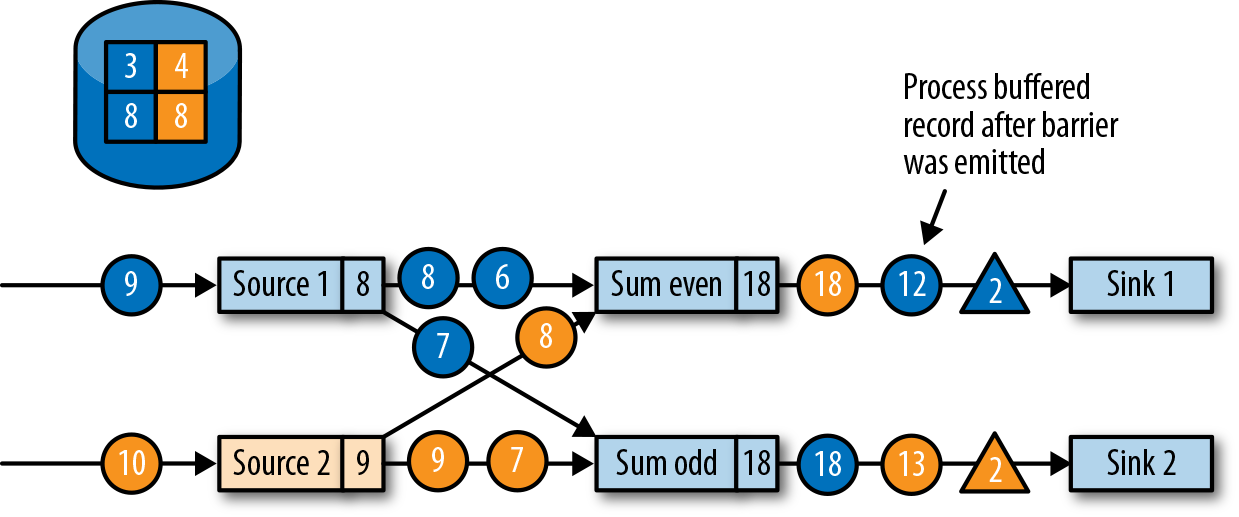
\includegraphics[width=0.7\textwidth]{images/spaf_0324.png}
    \caption{lambda架构}
\end{figure}

最终，检查点分界线会到达输出（sink）任务。当sink任务接收到barrier时，它也会先执行``分界线对齐''，然后将自己的状态保存到检查点，并向作业管理器确认已接收到barrier。一旦从应用程序的所有任务收到一个检查点的确认信息，作业管理器就会将这个检查点记录为已完成。图3-25显示了检查点算法的最后一步。这样，当发生故障时，我们就可以用已完成的检查点恢复应用程序了。

\begin{figure}[htbp]
    \centering
    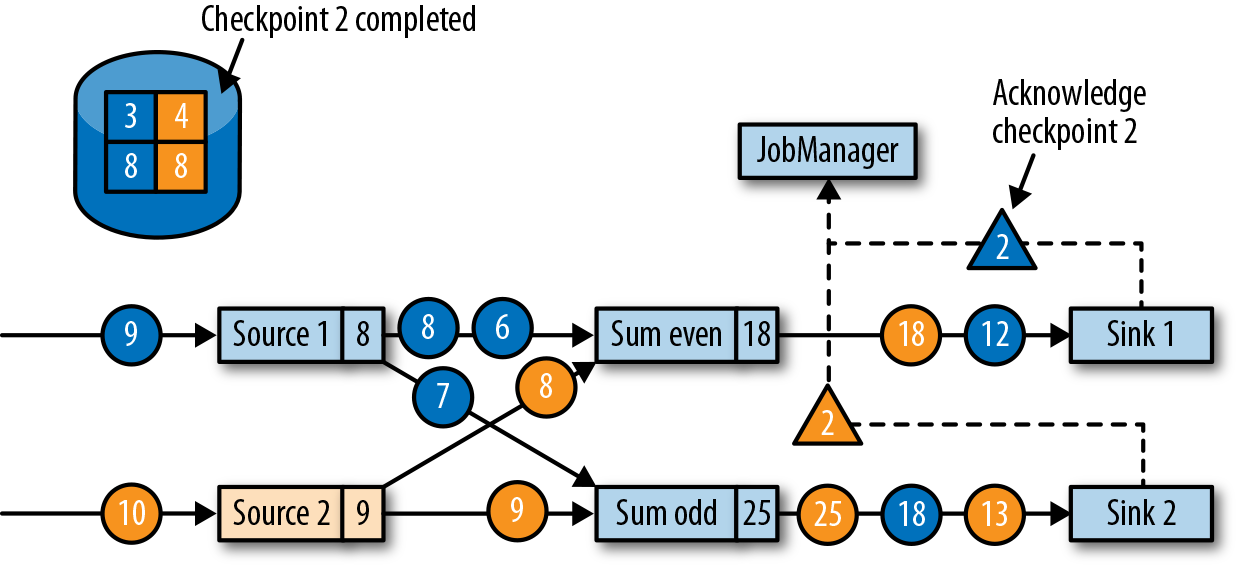
\includegraphics[width=0.7\textwidth]{images/spaf_0325.png}
    \caption{lambda架构}
\end{figure}

\subsection{检查点的性能影响}

Flink的检查点算法可以在不停止整个应用程序的情况下，生成一致的分布式检查点。但是，它可能会增加应用程序的处理延迟。Flink对此有一些调整措施，可以在某些场景下显得对性能的影响没那么大。

当任务将其状态保存到检查点时，它其实处于一个阻塞状态，而此时新的输入会被缓存起来。由于状态可能变得非常大，而且检查点需要通过网络将数据写入远程存储系统，检查点的写入很容易就会花费几秒到几分钟的时间——这对于要求低延迟的应用程序而言，显然是不可接受的。在Flink的设计中，真正负责执行检查点写入的，其实是状态后端。具体怎样复制任务的状态，取决于状态后端的实现方式。例如，文件系统（FileSystem）状态后端和RocksDB状态后端都支持了异步（asynchronous）检查点。触发检查点操作时，状态后端会先创建状态的本地副本。本地拷贝完成后，任务就将继续常规的数据处理，这往往并不会花费太多时间。一个后台线程会将本地快照异步复制到远程存储，并在完成检查点后再回来通知任务。异步检查点的机制，显著减少了任务继续处理数据之前的等待时间。此外，RocksDB状态后端还实现了增量的检查点，这样可以大大减少要传输的数据量。

为了减少检查点算法对处理延迟的影响，另一种技术是调整分界线对齐的步骤。对于需要非常低的延迟、并且可以容忍“至少一次”（at-least-once）状态保证的应用程序，Flink可以将检查点算法配置为，在等待barrier对齐期间处理所有到达的数据，而不是把barrier已经到达的那些分区的数据缓存起来。当检查点的所有barrier到达，算子任务就会将状态写入检查点——当然，现在的状态中，就可能包括了一些“提前”的更改，这些更改由本该属于下一个检查点的数据到来时触发。如果发生故障，从检查点恢复时，就将再次处理这些数据：这意味着检查点现在提供的是“至少一次”（at-least-once）而不是“精确一次”（exactly-once）的一致性保证。

\subsection{保存点}

Flink的恢复算法是基于状态检查点的。Flink根据可配置的策略，定期保存并自动丢弃检查点。检查点的目的是确保在发生故障时可以重新启动应用程序，所以当应用程序被显式地撤销（cancel）时，检查点会被删除掉。除此之外，应用程序状态的一致性快照还可用于除故障恢复之外的更多功能。

Flink中一个最有价值，也是最独特的功能是保存点（savepoints）。原则上，创建保存点使用的算法与检查点完全相同，因此保存点可以认为就是具有一些额外元数据的检查点。Flink不会自动创建保存点，因此用户（或者外部调度程序）必须明确地触发创建操作。同样，Flink也不会自动清理保存点。第10章将会具体介绍如何触发和处理保存点。

\textbf{使用保存点}

有了应用程序和与之兼容的保存点，我们就可以从保存点启动应用程序了。这会将应用程序的状态初始化为保存点的状态，并从保存点创建时的状态开始运行应用程序。虽然看起来这种行为似乎与用检查点从故障中恢复应用程序完全相同，但实际上故障恢复只是一种特殊情况，它只是在相同的集群上以相同的配置启动相同的应用程序。而从保存点启动应用程序会更加灵活，这就可以让我们做更多事情了。

\begin{itemize}
\item 可以从保存点启动不同但兼容的应用程序。这样一来，我们就可以及时修复应用程序中的逻辑bug，并让流式应用的源尽可能多地提供之前发生的事件，然后重新处理，以便修复之前的计算结果。修改后的应用程序还可用于运行A / B测试，或者具有不同业务逻辑的假设场景。这里要注意，应用程序和保存点必须兼容才可以这么做——也就是说，应用程序必须能够加载保存点的状态。
\item 可以使用不同的并行度来启动相同的应用程序，可以将应用程序的并行度增大或减小。
\item 可以在不同的集群上启动同样的应用程序。这非常有意义，意味着我们可以将应用程序迁移到较新的Flink版本或不同的集群上去。
\item 可以使用保存点暂停应用程序，稍后再恢复。这样做的意义在于，可以为更高优先级的应用程序释放集群资源，或者在输入数据不连续生成时释放集群资源。
\item 还可以将保存点设置为某一版本，并归档（archive）存储应用程序的状态。
\end{itemize}

保存点是非常强大的功能，所以许多用户会定期创建保存点以便能够及时退回之前的状态。我们见到的各种场景中，保存点一个最有趣的应用是不断将流应用程序迁移到更便宜的数据中心上去。

\textbf{从保存点启动应用程序}

前面提到的保存点的所有用例，都遵循相同的模式。那就是首先创建正在运行的应用程序的保存点，然后在一个新启动的应用程序中用它来恢复状态。之前我们已经知道，保存点的创建和检查点非常相似，而接下来我们就将介绍对于一个从保存点启动的应用程序，Flink如何初始化其状态。

应用程序由多个算子组成。每个算子可以定义一个或多个键控状态和算子状态。算子由一个或多个算子任务并行执行。因此，一个典型的应用程序会包含多个状态，这些状态分布在多个算子任务中，这些任务可以运行在不同的TaskManager进程上。

图3-26显示了一个具有三个算子的应用程序，每个算子执行两个算子任务。一个算子（OP-1）具有单一的算子状态（OS-1），而另一个算子（OP-2）具有两个键控状态（KS-1和KS-2）。当保存点创建时，会将所有任务的状态复制到持久化的存储位置。

保存点中的状态拷贝会以算子标识符（operator ID）和状态名称（state name）组织起来。算子ID和状态名称必须能够将保存点的状态数据，映射到一个正在启动的应用程序的算子状态。从保存点启动应用程序时，Flink会将保存点的数据重新分配给相应的算子任务。

\begin{note}
    请注意，保存点不包含有关算子任务的信息。这是因为当应用程序以不同的并行度启动时，任务数量可能会更改。
\end{note}

如果我们要从保存点启动一个修改过的应用程序，那么保存点中的状态只能映射到符合标准的应用程序——它里面的算子必须具有相应的ID和状态名称。默认情况下，Flink会自动分配唯一的算子ID。然而，一个算子的ID，是基于它之前算子的ID确定性地生成的。因此，算子的ID会在其前序算子改变时改变，比如，当我们添加了新的或移除掉一个算子时，前序算子ID改变，当前算子ID就会变化。所以对于具有默认算子ID的应用程序而言，如果想在不丢失状态的前提下升级，就会受到极大的限制。因此，我们强烈建议在程序中为算子手动分配唯一ID，而不是依靠Flink的默认分配。我们将在“指定唯一的算子标识符”一节中详细说明如何分配算子标识符。

\chapter{Flink DataStream API}

本章介绍了Flink DataStream API的基本知识。我们展示了典型的Flink流处理程序的结构和组成部分，还讨论了Flink的类型系统以及支持的数据类型，还展示了数据和分区转换操作。窗口操作符，基于时间语义的转换操作，有状态的操作符，以及和外部系统的连接器将在接下来的章节进行介绍。阅读完这一章后，我们将会知道如何去实现一个具有基本功能的流处理程序。我们的示例程序采用Scala语言，因为Scala语言相对比较简洁。但Java API也是十分类似的（特殊情况，我们将会指出）。在我们的Github仓库里，我们所写的应用程序具有Scala和Java两种版本。

\section{你好，Flink！}

让我们写一个简单的例子来获得使用DataStream API编写流处理应用程序的粗浅印象。我们将使用这个简单的示例来展示一个Flink程序的基本结构，以及介绍一些DataStream API的重要特性。我们的示例程序摄取了一条（来自多个传感器的）温度测量数据流。

首先让我们看一下表示传感器读数的数据结构：

\begin{minted}[linenos,breaklines,fontsize=\footnotesize]{java}
public class SensorReading {

    public String id;
    public long timestamp;
    public double temperature;

    public SensorReading() { }

    public SensorReading(String id, long timestamp, double temperature) {
        this.id = id;
        this.timestamp = timestamp;
        this.temperature = temperature;
    }

    public String toString() {
        return "(" + this.id + ", " + this.timestamp + ", " + this.temperature + ")";
    }
}
\end{minted}

示例程序将温度从华氏温度读数转换成摄氏温度读数，然后针对每一个传感器，每5秒钟计算一次平均温度纸。

\begin{minted}[linenos,breaklines,fontsize=\footnotesize]{java}
public class AverageSensorReadings {
  public static void main(String[] args) throws Exception {
    final StreamExecutionEnvironment env = StreamExecutionEnvironment.getExecutionEnvironment();
    env.setStreamTimeCharacteristic(TimeCharacteristic.EventTime);

    DataStream<SensorReading> sensorData = env.addSource(new SensorSource());

    DataStream<T> avgTemp = sensorData
      .map(r -> {
        Double celsius = (r.temperature - 32) * (5.0 / 9.0);
        return SensorReading(r.id, r.timestamp, celsius);
      })
      .keyBy(r -> r.id)
      .timeWindow(Time.seconds(5))
      .apply(new TemperatureAverager());

    avgTemp.print();

    env.execute("Compute average sensor temperature");
  }
}
\end{minted}

你可能已经注意到Flink程序的定义和提交执行使用的就是正常的Java的方法。大多数情况下，这些代码都写在一个静态main方法中。在我们的例子中，我们定义了AverageSensorReadings对象，然后将大多数的应用程序逻辑放在了main()中。

Flink流处理程序的结构如下：

\begin{enumerate}
    \item 创建Flink程序执行环境。
    \item 从数据源读取一条或者多条流数据
    \item 使用流转换算子实现业务逻辑
    \item 将计算结果输出到一个或者多个外部设备（可选）
    \item 执行程序
\end{enumerate}

接下来我们详细的学习一下这些部分。

\section{搭建执行环境}

编写Flink程序的第一件事情就是搭建执行环境。执行环境决定了程序是运行在单机上还是集群上。在DataStream API中，程序的执行环境是由StreamExecutionEnvironment设置的。在我们的例子中，我们通过调用静态getExecutionEnvironment()方法来获取执行环境。这个方法根据调用方法的上下文，返回一个本地的或者远程的环境。如果这个方法是一个客户端提交到远程集群的代码调用的，那么这个方法将会返回一个远程的执行环境。否则，将返回本地执行环境。

也可以用下面的方法来显式的创建本地或者远程执行环境：

\begin{minted}[linenos,breaklines,fontsize=\footnotesize]{java}
StreamExecutionEnvironment localEnv = StreamExecutionEnvironment
  .createLocalEnvironment();

StreamExecutionEnvironment remoteEnv = StreamExecutionEnvironment
  .createRemoteEnvironment(
    "host", // hostname of JobManager
    1234, // port of JobManager process
    "path/to/jarFile.jar"
  ); // JAR file to ship to the JobManager
\end{minted}

接下来，我们使用env.setStreamTimeCharacteristic(TimeCharacteristic.EventTime)来将我们程序的时间语义设置为事件时间。执行环境提供了很多配置选项，例如：设置程序的并行度和程序是否开启容错机制。

\section{读取输入流}

一旦执行环境设置好，就该写业务逻辑了。StreamExecutionEnvironment提供了创建数据源的方法，这些方法可以从数据流中将数据摄取到程序中。数据流可以来自消息队列或者文件系统，也可能是实时产生的（例如socket）。

在我们的例子里面，我们这样写：

\begin{minted}[linenos,breaklines,fontsize=\footnotesize]{java}
DataStream<SensorReading> sensorData = env
  .addSource(new SensorSource());
\end{minted}

这样就可以连接到传感器测量数据的数据源并创建一个类型为SensorReading的DataStream了。Flink支持很多数据类型，我们将在接下来的章节里面讲解。在我们的例子里面，我们的数据类型是一个定义好的Scala样例类。SensorReading样例类包含了传感器ID，数据的测量时间戳，以及测量温度值。assignTimestampsAndWatermarks(new SensorTimeAssigner)方法指定了如何设置事件时间语义的时间戳和水位线。有关SensorTimeAssigner我们后面再讲。

\section{转换算子的使用}

一旦我们有一条DataStream，我们就可以在这条数据流上面使用转换算子了。转换算子有很多种。一些转换算子可以产生一条新的DataStream，当然这个DataStream的类型可能是新类型。还有一些转换算子不会改变原有DataStream的数据，但会将数据流分区或者分组。业务逻辑就是由转换算子串起来组合而成的。

在我们的例子中，我们首先使用map()转换算子将传感器的温度值转换成了摄氏温度单位。然后，我们使用keyBy()转换算子将传感器读数流按照传感器ID进行分区。接下来，我们定义了一个timeWindow()转换算子，这个算子将每个传感器ID所对应的分区的传感器读数分配到了5秒钟的滚动窗口中。

\begin{minted}[linenos,breaklines,fontsize=\footnotesize]{java}
DataStream<T> avgTemp = sensorData
  .map(r -> {
    Double celsius = (r.temperature -32) * (5.0 / 9.0);
    return SensorReading(r.id, r.timestamp, celsius);
  })
  .keyBy(r -> r.id)
  .timeWindow(Time.seconds(5))
  .apply(new TemperatureAverager());
\end{minted}

窗口转换算子将在“窗口操作符”一章中讲解。最后，我们使用了一个UDF函数来计算每个窗口的温度的平均值。我们稍后将会讨论UDF函数的实现。

\section{输出结果}

流处理程序经常将它们的计算结果发送到一些外部系统中去，例如：Apache Kafka，文件系统，或者数据库中。Flink提供了一个维护的很好的sink算子的集合，这些sink算子可以用来将数据写入到不同的系统中去。我们也可以实现自己的sink算子。也有一些Flink程序并不会向第三方外部系统发送数据，而是将数据存储到Flink系统内部，然后可以使用Flink的可查询状态的特性来查询数据。

在我们的例子中，计算结果是一个DataStream<SensorReading>数据记录。每一条数据记录包含了一个传感器在5秒钟的周期里面的平均温度。计算结果组成的数据流将会调用print()将计算结果写到标准输出。

\begin{minted}[linenos,breaklines,fontsize=\footnotesize]{java}
avgTemp.print();
\end{minted}

\begin{note}
    要注意一点，流的Sink算子的选择将会影响应用程序端到端(end-to-end)的一致性，具体就是应用程序的计算提供的到底是at-least-once还是exactly-once的一致性语义。应用程序端到端的一致性依赖于所选择的流的Sink算子和Flink的检查点算法的集成使用。
\end{note}

\section{执行}

当应用程序完全写好时，我们可以调用StreamExecutionEnvironment.execute()来执行应用程序。在我们的例子中就是我们的最后一行调用：

\begin{minted}[linenos,breaklines,fontsize=\footnotesize]{java}
env.execute("Compute average sensor temperature");
\end{minted}

Flink程序是惰性执行的。也就是说创建数据源和转换算子的API调用并不会立刻触发任何数据处理逻辑。API调用仅仅是在执行环境中构建了一个执行计划，这个执行计划包含了执行环境创建的数据源和所有的将要用在数据源上的转换算子。只有当execute()被调用时，系统才会触发程序的执行。

构建好的执行计划将被翻译成一个JobGraph并提交到JobManager上面去执行。根据执行环境的种类，一个JobManager将会运行在一个本地线程中（如果是本地执行环境的化）或者JobGraph将会被发送到一个远程的JobManager上面去。如果JobManager远程运行，那么JobGraph必须和一个包含有所有类和应用程序的依赖的JAR包一起发送到远程JobManager。

\section{自定义产生传感器读数的数据源}

\begin{minted}[linenos,breaklines,fontsize=\footnotesize]{java}
public class SensorSource extends RichParallelSourceFunction<SensorReading> {

    private boolean running = true;

    @Override
    public void run(SourceContext<SensorReading> srcCtx) throws Exception {

        Random rand = new Random();

        String[] sensorIds = new String[10];
        double[] curFTemp = new double[10];
        for (int i = 0; i < 10; i++) {
            sensorIds[i] = "sensor_" + i;
            curFTemp[i] = 65 + (rand.nextGaussian() * 20);
        }

        while (running) {
            long curTime = Calendar.getInstance().getTimeInMillis();
            for (int i = 0; i < 10; i++) {
                curFTemp[i] += rand.nextGaussian() * 0.5;
                srcCtx.collect(new SensorReading(sensorIds[i], curTime, curFTemp[i]));
            }

            Thread.sleep(100);
        }
    }

    @Override
    public void cancel() {
        this.running = false;
    }
}
\end{minted}

使用方法

\begin{minted}[linenos,breaklines,fontsize=\footnotesize]{java}
DataStream<SensorReading> sensorData = env.addSource(new SensorSource());
\end{minted}

\section{转换算子}

在这一小节我们将大概看一下DataStream API的基本转换算子。与时间有关的操作符（例如窗口操作符和其他特殊的转换算子）将会在后面的章节叙述。一个流的转换操作将会应用在一个或者多个流上面，这些转换操作将流转换成一个或者多个输出流。编写一个DataStream API简单来说就是将这些转换算子组合在一起来构建一个数据流图，这个数据流图就实现了我们的业务逻辑。

大部分的流转换操作都基于用户自定义函数UDF。UDF函数打包了一些业务逻辑并定义了输入流的元素如何转换成输出流的元素。像MapFunction这样的函数，将会被定义为类，这个类实现了Flink针对特定的转换操作暴露出来的接口。

\begin{minted}[linenos,breaklines,fontsize=\footnotesize]{java}
DataStream<String> sensorIds = filteredReadings.map(r -> r.id);
\end{minted}

函数接口定义了需要由用户实现的转换方法，例如上面例子中的map()方法。

大部分函数接口被设计为Single Abstract Method（单独抽象方法）接口，并且接口可以使用Java 8匿名函数来实现。Scala DataStream API也内置了对匿名函数的支持。当讲解DataStream API的转换算子时，我们展示了针对所有函数类的接口，但为了简洁，大部分接口的实现使用匿名函数而不是函数类的方式。

DataStream API针对大多数数据转换操作提供了转换算子。如果你很熟悉批处理API、函数式编程语言或者SQL，那么你将会发现这些API很容易学习。我们会将DataStream API的转换算子分成四类：

\begin{itemize}
    \item 基本转换算子：将会作用在数据流中的每一条单独的数据上。
    \item KeyedStream转换算子：在数据有key的情况下，对数据应用转换算子。
    \item 多流转换算子：合并多条流为一条流或者将一条流分割为多条流。
    \item 分布式转换算子：将重新组织流里面的事件。
\end{itemize}

\subsection{基本转换算子}

基本转换算子会针对流中的每一个单独的事件做处理，也就是说每一个输入数据会产生一个输出数据。单值转换，数据的分割，数据的过滤，都是基本转换操作的典型例子。我们将解释这些算子的语义并提供示例代码。

\textit{MAP}

map算子通过调用DataStream.map()来指定。map算子的使用将会产生一条新的数据流。它会将每一个输入的事件传送到一个用户自定义的mapper，这个mapper只返回一个输出事件，这个输出事件和输入事件的类型可能不一样。图5-1展示了一个map算子，这个map将每一个正方形转化成了圆形。

\begin{figure}[htbp]
    \centering
    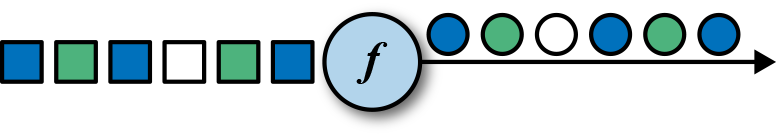
\includegraphics[width=0.7\textwidth]{images/spaf_0501.png}
    \caption{lambda架构}
\end{figure}

MapFunction的类型与输入事件和输出事件的类型相关，可以通过实现MapFunction接口来定义。接口包含map()函数，这个函数将一个输入事件恰好转换为一个输出事件。

\begin{minted}[linenos,breaklines,fontsize=\footnotesize]{java}
// T: the type of input elements
// O: the type of output elements
MapFunction[T, O]
    > map(T): O
\end{minted}

下面的代码实现了将SensorReading中的id字段抽取出来的功能。

\begin{minted}[linenos,breaklines,fontsize=\footnotesize]{java}
DataStream<SensorReading> readings = ...
DataStream<String> sensorIds = readings.map(new IdExtractor());

public static class IdExtractor implements MapFunction<SensorReading, String> {
    @Override
    public String map(SensorReading r) throws Exception {
        return r.id;
    }
}
\end{minted}

当然我们更推荐匿名函数的写法。

\begin{minted}[linenos,breaklines,fontsize=\footnotesize]{java}
DataStream<String> sensorIds = filteredReadings.map(r -> r.id);
\end{minted}

\textit{FILTER}

filter转换算子通过在每个输入事件上对一个布尔条件进行求值来过滤掉一些元素，然后将剩下的元素继续发送。一个true的求值结果将会把输入事件保留下来并发送到输出，而如果求值结果为false，则输入事件会被抛弃掉。我们通过调用DataStream.filter()来指定流的filter算子，filter操作将产生一条新的流，其类型和输入流中的事件类型是一样的。图5-2展示了只产生白色方框的filter操作。

\begin{figure}[htbp]
    \centering
    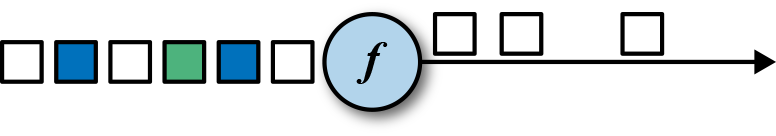
\includegraphics[width=0.7\textwidth]{images/spaf_0502.png}
    \caption{lambda架构}
\end{figure}

布尔条件可以使用函数、FilterFunction接口或者匿名函数来实现。FilterFunction中的泛型是输入事件的类型。定义的filter()方法会作用在每一个输入元素上面，并返回一个布尔值。

\begin{minted}[linenos,breaklines,fontsize=\footnotesize]{java}
// T: the type of elements
FilterFunction[T]
    > filter(T): Boolean
\end{minted}

下面的例子展示了如何使用filter来从传感器数据中过滤掉温度值小于25华氏温度的读数。

\begin{minted}[linenos,breaklines,fontsize=\footnotesize]{java}
DataStream<SensorReading> filteredReadings = readings.filter(r -> r.temperature >= 25);
\end{minted}

\textit{FLATMAP}

flatMap算子和map算子很类似，不同之处在于针对每一个输入事件flatMap可以生成0个、1个或者多个输出元素。事实上，flatMap转换算子是filter和map的泛化。所以flatMap可以实现map和filter算子的功能。图5-3展示了flatMap如何根据输入事件的颜色来做不同的处理。如果输入事件是白色方框，则直接输出。输入元素是黑框，则复制输入。灰色方框会被过滤掉。

\begin{figure}[htbp]
    \centering
    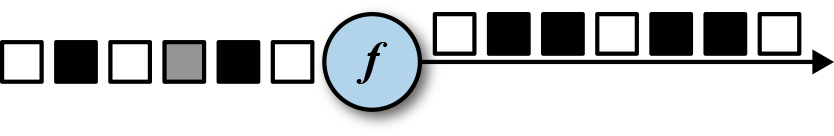
\includegraphics[width=0.7\textwidth]{images/spaf_0503.png}
    \caption{lambda架构}
\end{figure}

flatMap算子将会应用在每一个输入事件上面。对应的FlatMapFunction定义了flatMap()方法，这个方法返回0个、1个或者多个事件到一个Collector集合中，作为输出结果。

\begin{minted}[linenos,breaklines,fontsize=\footnotesize]{java}
// T: the type of input elements
// O: the type of output elements
FlatMapFunction[T, O]
    > flatMap(T, Collector[O]): Unit
\end{minted}

下面的例子展示了在数据分析教程中经常用到的例子，我们用flatMap来实现。使用\_来切割传感器ID，比如sensor\_1。

\begin{minted}[linenos,breaklines,fontsize=\footnotesize]{java}
public static class IdSplitter implements FlatMapFunction<String, String> {
    @Override
    public void flatMap(String id, Collector<String> out) {

        String[] splits = id.split("_");

        for (String split : splits) {
            out.collect(split);
        }
    }
}
\end{minted}

匿名函数写法：

\begin{minted}[linenos,breaklines,fontsize=\footnotesize]{java}
DataStream<String> splitIds = sensorIds
    .flatMap((FlatMapFunction<String, String>)
            (id, out) -> { for (String s: id.split("_")) { out.collect(s);}})
    // provide result type because Java cannot infer return type of lambda function
    // 提供结果的类型，因为Java无法推断匿名函数的返回值类型
    .returns(Types.STRING);
\end{minted}

\subsection{键控流转换算子}

很多流处理程序的一个基本要求就是要能对数据进行分组，分组后的数据共享某一个相同的属性。DataStream API提供了一个叫做KeyedStream的抽象，此抽象会从逻辑上对DataStream进行分区，分区后的数据拥有同样的Key值，分区后的流互不相关。

针对KeyedStream的状态转换操作可以读取数据或者写入数据到当前事件Key所对应的状态中。这表明拥有同样Key的所有事件都可以访问同样的状态，也就是说所以这些事件可以一起处理。

\begin{note}
    要小心使用状态转换操作和基于Key的聚合操作。如果Key的值越来越多，例如：Key是订单ID，我们必须及时清空Key所对应的状态，以免引起内存方面的问题。稍后我们会详细讲解。
\end{note}

KeyedStream可以使用map，flatMap和filter算子来处理。接下来我们会使用keyBy算子来将DataStream转换成KeyedStream，并讲解基于key的转换操作：滚动聚合和reduce算子。

\textit{KEYBY}

keyBy通过指定key来将DataStream转换成KeyedStream。基于不同的key，流中的事件将被分配到不同的分区中去。所有具有相同key的事件将会在接下来的操作符的同一个子任务槽中进行处理。拥有不同key的事件可以在同一个任务中处理。但是算子只能访问当前事件的key所对应的状态。

如图5-4所示，把输入事件的颜色作为key，黑色的事件输出到了一个分区，其他颜色输出到了另一个分区。

\begin{figure}[htbp]
    \centering
    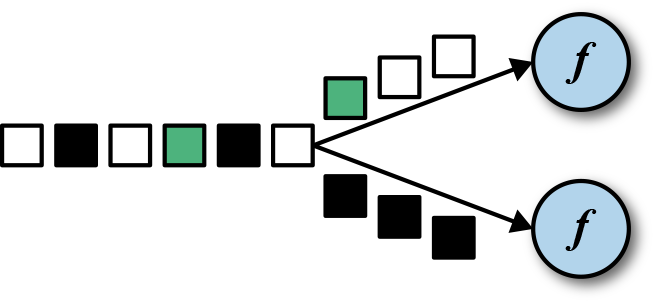
\includegraphics[width=0.7\textwidth]{images/spaf_0504.png}
    \caption{lambda架构}
\end{figure}

keyBy()方法接收一个参数，这个参数指定了key或者keys，有很多不同的方法来指定key。我们将在后面讲解。下面的代码声明了id这个字段为SensorReading流的key。

\begin{minted}[linenos,breaklines,fontsize=\footnotesize]{java}
KeyedStream<SensorReading, String> keyed = readings.keyBy(r -> r.id);
\end{minted}

匿名函数r -> r.id抽取了传感器读数SensorReading的id值。

\textit{滚动聚合}

滚动聚合算子由KeyedStream调用，并生成一个聚合以后的DataStream，例如：sum，minimum，maximum。一个滚动聚合算子会为每一个观察到的key保存一个聚合的值。针对每一个输入事件，算子将会更新保存的聚合结果，并发送一个带有更新后的值的事件到下游算子。滚动聚合不需要用户自定义函数，但需要接受一个参数，这个参数指定了在哪一个字段上面做聚合操作。DataStream API提供了以下滚动聚合方法。

\begin{note}
    滚动聚合算子只能用在滚动窗口，不能用在滑动窗口。
\end{note}

\begin{itemize}
    \item sum()：在输入流上对指定的字段做滚动相加操作。
    \item min()：在输入流上对指定的字段求最小值。
    \item max()：在输入流上对指定的字段求最大值。
    \item minBy()：在输入流上针对指定字段求最小值，并返回包含当前观察到的最小值的事件。
    \item maxBy()：在输入流上针对指定字段求最大值，并返回包含当前观察到的最大值的事件。
\end{itemize}

滚动聚合算子无法组合起来使用，每次计算只能使用一个单独的滚动聚合算子。

下面的例子根据第一个字段来对类型为Tuple3<Int, Int, Int>的流做分流操作，然后针对第二个字段做滚动求和操作。

\begin{minted}[linenos,breaklines,fontsize=\footnotesize]{java}
DataStream<Tuple3<Integer, Integer, Integer>> inputStream = env.fromElements(new Tuple3(1, 2, 2), new Tuple3(2, 3, 1), new Tuple3(2, 2, 4), new Tuple3(1, 5, 3));

DataStream<Tuple3<Integer, Integer, Integer>> resultStream = inputStream
  .keyBy(0) // key on first field of the tuple
  .sum(1);   // sum the second field of the tuple in place
\end{minted}

在这个例子里面，输入流根据第一个字段来分流，然后在第二个字段上做计算。对于key 1，输出结果是(1,2,2),(1,7,2)。对于key 2，输出结果是(2,3,1),(2,5,1)。第一个字段是key，第二个字段是求和的数值，第三个字段未定义。

\begin{note}
    滚动聚合操作会对每一个key都保存一个状态。因为状态从来不会被清空，所以我们在使用滚动聚合算子时只能使用在含有有限个key的流上面。
\end{note}

\textit{REDUCE}

reduce算子是滚动聚合的泛化实现。它将一个ReduceFunction应用到了一个KeyedStream上面去。reduce算子将会把每一个输入事件和当前已经reduce出来的值做聚合计算。reduce操作不会改变流的事件类型。输出流数据类型和输入流数据类型是一样的。

reduce函数可以通过实现接口ReduceFunction来创建一个类。ReduceFunction接口定义了reduce()方法，此方法接收两个输入事件，输入一个相同类型的事件。

\begin{minted}[linenos,breaklines,fontsize=\footnotesize]{java}
// T: the element type
ReduceFunction[T]
    > reduce(T, T): T
\end{minted}

下面的例子，流根据传感器ID分流，然后计算每个传感器的当前最大温度值。

\begin{minted}[linenos,breaklines,fontsize=\footnotesize]{java}
DataStream<SensorReading> maxTempPerSensor = keyed
        .reduce((r1, r2) -> {
            if (r1.temperature > r2.temperature) {
                return r1;
            } else {
                return r2;
            }
        });
\end{minted}

\begin{note}
    reduce作为滚动聚合的泛化实现，同样也要针对每一个key保存状态。因为状态从来不会清空，所以我们需要将reduce算子应用在一个有限key的流上。
\end{note}

\subsection{多流转换算子}

许多应用需要摄入多个流并将流合并处理，还可能需要将一条流分割成多条流然后针对每一条流应用不同的业务逻辑。接下来，我们将讨论DataStream API中提供的能够处理多条输入流或者发送多条输出流的操作算子。

\textit{UNION}

DataStream.union()方法将两条或者多条DataStream合并成一条具有与输入流相同类型的输出DataStream。接下来的转换算子将会处理输入流中的所有元素。图5-5展示了union操作符如何将黑色和白色的事件流合并成一个单一输出流。



















\chapter{Elegant\LaTeX{} 系列模板介绍}

Elegant\LaTeX{} 项目组致力于打造一系列美观、优雅、简便的模板方便用户使用。目前由 \href{https://github.com/ElegantLaTeX/ElegantNote}{ElegantNote}，\href{https://github.com/ElegantLaTeX/ElegantBook}{ElegantBook}，\href{https://github.com/ElegantLaTeX/ElegantPaper}{ElegantPaper} 组成，分别用于排版笔记，书籍和工作论文。强烈推荐使用最新正式版本！本文将介绍本模板的一些设置内容以及基本使用方法。如果您有其他问题，建议或者意见，欢迎在 GitHub 上给我们提交 \href{https://github.com/ElegantLaTeX/ElegantBook/issues}{issues} 或者邮件联系我们。

我们的联系方式如下，建议加入用户 QQ 群提问，这样能更快获得准确的反馈，加群时请备注 \LaTeX{} 或者 Elegant\LaTeX{} 相关内容。
\begin{itemize}
  \item 官网：\href{https://elegantlatex.org/}{https://elegantlatex.org/}
  \item GitHub 网址：\href{https://github.com/ElegantLaTeX/}{https://github.com/ElegantLaTeX/}
  \item CTAN 地址：\href{https://ctan.org/pkg/elegantbook}{https://ctan.org/pkg/elegantbook}
  \item 文档 Wiki：\href{https://github.com/ElegantLaTeX/ElegantBook/wiki}{https://github.com/ElegantLaTeX/ElegantBook/wiki}
  \item 下载地址：\href{https://github.com/ElegantLaTeX/ElegantBook/releases}{正式发行版}，\href{https://github.com/ElegantLaTeX/ElegantBook/archive/master.zip}{最新版}
  \item 微博：Elegant\LaTeX{}
  \item 微信公众号：Elegant\LaTeX{}
  \item 用户 QQ 群：692108391 
  \item 邮件：\email{elegantlatex2e@gmail.com}
\end{itemize}


\section{ElegantBook 更新说明}

此次为 3.x 最后一个版本，在 3.10 基础上，主要为了解决 \TeX{} Live 2020 中编译错误，具体内容有：

\begin{enumerate}
  \item \textbf{重要修正}：修复因为 \lstinline{gbt7714} 宏包更新导致的 \lstinline{natbib option clash} 错误；
  \item 由于 \lstinline{pgfornament} 宏包未被 \TeX Live 2020 收录，因此删除 base 相关的内容；
  \item 修复部分环境的空格问题；
  \item 增加了意大利语言选项 \lstinline{lang=it}。
\end{enumerate}

\begin{note}
如果你使用旧版本切换到新版本时，遇到问题时，请核对文档中是否有 \lstinline{pageanchor} 字样。如果有，请删除文档中的 \lstinline|\hypersetup{pageanchor=true}|，并且在 \lstinline{\maketitle} 和 \lstinline{\tableofcontents} 之间添加 \lstinline{\frontmatter}。2.x 版本的用户请仔细查看\href{https://github.com/ElegantLaTeX/ElegantBook/wiki/convert}{跨版本转换}。
\end{note}

\section{模板安装与更新}

你可以通过免安装的方式使用本模板，包括在线使用和本地（文件夹内）使用两种方式，也可以通过 \TeX{} 发行版安装使用。

\subsection{在线使用模板}

我们把三套模板全部上传到 \href{https://www.overleaf.com/}{Overleaf} 上了，网络便利的用户可以直接通过 Overleaf 在线使用我们的模板。使用 Overleaf 的好处是无需安装 \TeX{} Live 2020，可以随时随地访问自己的文件。查找模板，请在 Overleaf 模板库里面搜索 \lstinline{elegantlatex} 即可，你也可以直接访问\href{https://www.overleaf.com/latex/templates?addsearch=elegantlatex}{搜索结果}。选择适当的模板之后，将其 \lstinline{Open as Template}，即可把模板存到自己账户下，然后可以自由编辑以及与别人一起协作。更多关于 Overleaf 的介绍和使用，请参考 Overleaf 的\href{https://www.overleaf.com/learn}{官方文档}。

\begin{remark}
Overleaf 上，中文需要使用 \hologo{XeLaTeX} 进行编译，英文建议使用 \hologo{pdfLaTeX} 编译。
\end{remark}

\subsection{本地免安装使用}


\textbf{免安装}使用方法如下，从 GitHub 或者 CTAN 下载最新（正式）版文件，严格意义上只需要类文件 \lstinline{elegantbook.cls}。然后将模板文件放在你的工作目录下即可使用。这样使用的好处是，无需安装，简便；缺点是，当模板更新之后，你需要手动替换 \lstinline{cls} 文件。

\subsection{发行版安装使用}

如果你是 \TeX{} Live 2019 用户，我们推荐你直接进行安装和更新。你可以通过 \TeX{} Live 2019 自带的 \lstinline{tlshell}\footnote{也叫 \TeX{} Live Manager} 进行安装。安装非常简单，步骤如下，搜索并打开 \lstinline{tlshell}，然后通过 \lstinline{File -> Load Default Repository} 加载远程仓库，如果你不想使用默认的仓库，你可以通过 \lstinline{Options} 下的菜单设置远程仓库。设置好仓库之后，等待仓库加载完毕，你可以在下面的搜索栏搜索 \lstinline{elegantbook}，然后选择进行安装与更新。

\begin{figure}[htbp]
  \centering
  
\includegraphics[width=0.7\textwidth]{tlshell.png}
  \caption{使用 \TeX{} Live Shell 安装 ElegantBook 模板}
\end{figure}

\subsection{更新问题}

如果使用 \lstinline{tlshell} 无法更新模板，请使用命令行全部更新全部宏包或者使用免安装的方法使用本模板。

通过命令行（管理员权限）输入下面的命令对 tlmgr 自身和全部宏包进行更新。

\begin{lstlisting}
  tlmgr update --self 
  tlmgr update --all
\end{lstlisting}

更多的内容请参考 \href{https://tex.stackexchange.com/questions/55437/how-do-i-update-my-tex-distribution}{How do I update my \TeX{} distribution?}

\subsection{其他发行版本}

如果你是 \TeX{} Live 2018 的用户，由于 2018 难以更新到 2019，建议卸载 2018 重装 2019。如果嫌麻烦，你可以手动安装模板，将 \lstinline{elegantbook.cls} 复制到你的 \TeX{} Live 目录下，默认安装目录为 \lstinline|C:\texlive\2019\texmf-dist\tex\latex\elegantbook|，然后通过命令行（管理员权限），运行 \lstinline{texhash} 即可。

由于宏包版本问题，本模板不支持 C\TeX{} 套装。更多关于 \TeX{} Live 2019 的安装使用以及 C\TeX{} 与 \TeX{} Live 的兼容、系统路径问题，请参考官方文档以及啸行的\href{https://github.com/OsbertWang/install_latex/releases}{一份简短的安装 \LaTeX{} 的介绍}。


\section{用户作品计划}

Elegant\LaTeX{} 系列模板从创立至今已经有 9 年了，我们的模板也受到了很多用户的喜爱，在此，为了促进模板用户之间的交流，了解用户需求，完善本模板，我们将建立一个区域专门展示用户的文档，包括但不限于 GitHub 和官网等。如果你愿意将自己的作品展示出来，请邮件或者其他方式联系我们。如果自己代码已经传到 GitHub 或者 Gitee 等网站，可以提供对应网址。\href{https://github.com/ElegantLaTeX/Archive/tree/master/Collections}{用户文档中心}目前有下面一些作品：
\begin{enumerate}
\item 唐绍东：微积分笔记
\item 曲豆豆：超甜微积分习题集
\item 王世强：《化工数值计算与 MATLAB》复习指南
\item 李晨迪：Fluid Mechanics Notes
\item 肖明顺：地球物理勘查常用规范汇编
\item 白衣卿相：期末复习笔记-拓扑学摘要
\end{enumerate}

\section{关于提交}

出于某些因素的考虑，Elegant\LaTeX{} 项目自 2019 年 5 月 20 日开始，\textbf{不再接受任何非作者预约性质的提交}（pull request)！如果你想改进模板，你可以给我们提交 issues，或者可以在遵循协议（LPPL-1.3c）的情况下，克隆到自己仓库下进行修改。

\section{协作人员招募}

招募 Elegant\LaTeX{} 的协作人员（志愿者），没有报酬。工作内容：翻译 Elegant\LaTeX{} 系列模板文档，维护模板的维基，如果有公众号文稿写作经历的话，也可以帮忙写微信稿。本公告长期有效。目前 Elegant\LaTeX{} 共有 4 名协作人员，在此感谢他们无私的奉献！
\begin{itemize}
  \item 官方文档翻译: \href{https://github.com/peggy2006xzyz}{YPY};
  \item GitHub 维基维护: \href{https://github.com/izinngo}{Ingo Zinngo}、\href{https://github.com/xiaohao890809}{追寻原风景};
  \item QQ 群管理、FAQ 整理: \href{https://github.com/sikouhjw}{Sikouhjw}.
\end{itemize}

另外，也感谢 \href{https://github.com/stone-zeng}{Xiangdong Zeng}、\href{https://github.com/latexers}{逐鹿人}等人帮忙群管理。

\section{致谢}
2019 年 5 月 20 日，ElegantBook 模板在 GitHub 上的收藏数（star）达到了 100\footnote{截止 3.10 版本正式发布，star 数为 374。}。在此特别感谢 China\TeX{} 以及 \href{http://www.latexstudio.net/}{\LaTeX{} 工作室}对于本系列模板的大力宣传与推广。\LaTeX{} 工作室网站上有很多精彩的帖子和精致的模板，欢迎大家去挖掘里面的宝藏，这也是国内最全面的 \LaTeX{} 相关的网站。

如果你喜欢我们的模板，你可以在 GitHub 上收藏我们的模板。
%\begin{figure}[htbp]
%  \centering
%  \includegraphics[width=\textwidth]{star.png}
%  \caption{一键三连求赞}
%\end{figure}

\section{捐赠}

如果您非常喜爱我们的模板或者我，你还可以选择捐赠\footnote{最好在捐赠时备注信息。}以表达您对我们模板和我的支持。本模板自 3.08 版本发布了捐赠信息之后，收到了超过 1500 元的捐赠（四舍五入就是一个亿），非常感谢！

\begin{figure}[htbp]
\centering

\includegraphics[width=0.5\textwidth]{donate.jpg}
\end{figure}

\textbf{赞赏费用的使用解释权归 Elegant\LaTeX{} 所有，并且不接受监督，请自愿理性打赏}。10 元以上的赞赏，我们将列入捐赠榜，谢谢各位金主！

\begin{table}[!htb]
  \centering
  \caption{Elegant\LaTeX{} 系列模板捐赠榜}
    \begin{tabular}{*{4}{>{\scriptsize}c}|*{4}{>{\scriptsize}c}}
    \hline
    \textbf{捐赠者} & \textbf{金额} & \textbf{时间} & \textbf{渠道} & \textbf{捐赠者} & \textbf{金额} & \textbf{时间} & \textbf{渠道} \\
    \hline
    Lerh  & 10 RMB & 2019/05/15 & 微信    & 越过地平线 & 10 RMB & 2019/05/15 & 微信 \\
    银桑    & 20 RMB & 2019/05/27 & 微信    & *空    & 10 RMB & 2019/05/30 & 微信 \\
    latexstudio.net & 666 RMB & 2019/06/05 & 支付宝   & A*n   & 40 RMB & 2019/06/15 & 微信 \\
    * 夏   & 22 RMB & 2019/06/15 & 微信    & * 倩   & 21 RMB  & 2019/06/15 & 微信 \\
    Cassis & 11 RMB & 2019/06/30 & 微信    & *君    & 10 RMB & 2019/07/23 & 微信 \\
    P*u   & 50 RMB & 2019/07/30 & 微信    & *萌    & 19 RMB & 2019/08/28 & 微信 \\
    曲豆豆   & 10 RMB & 2019/08/28 & 微信    & 李博    & 100 RMB & 2019/10/06 & 微信 \\
    Njustsll & 10 RMB & 2019/10/11 & 微信    & 刘志阔   & 99.99 RMB & 2019/10/15 & 支付宝 \\
    * 韬   & 16 RMB & 2019/10/17 & 微信    & 赤霓    & 12 RMB & 2019/10/17 & 支付宝 \\
    追寻原风景 & 10 RMB & 2019/10/28 & 微信    & 郭德良   & 88 RMB & 2019/11/03 & 微信 \\
    自强不息  & 20 RMB & 2019/11/04 & 支付宝   & 读书之虫  & 20 RMB & 2019/11/18 & 微信 \\
    *等    & 10 RMB & 2019/11/18 & 微信    & *哲    & 20 RMB & 2019/11/18 & 微信 \\
    佚名    & 10 RMB & 2019/11/24 & 微信    & Jiye Qian & 66 RMB & 2019/12/04 & 微信 \\
    * 阳   & 20 RMB & 2019/12/05 & 微信    & Catcher & 11 RMB & 2019/12/08 & 支付宝 \\
    希尔波特门徒 & 10 RMB & 2019/12/09 & 支付宝   & * 伟   & 10 RMB & 2019/12/09 & 微信 \\
    Simon & 20 RMB & 2019/12/11 & 支付宝   & 流殇丶浅忆 & 66.60 RMB & 2019/12/18 & 支付宝 \\
    羽     & 10 RMB & 2019/12/20 & 支付宝   & * 琛   & 15 RMB & 2019/12/20 & 微信 \\
    随风    & 20 RMB & 2019/12/27 & 支付宝   & Ws    & 23.30 RMB & 2019/12/28 & 微信 \\
    初八    & 100 RMB  & 2020/01/02 & 支付宝   & p*e   & 20 RMB & 2020/01/03 & 微信 \\
    Shunmx & 100 RMB & 2020/01/03 & 微信    & hj    & 10 RMB & 2020/01/03 & 微信 \\
    F*5   & 10 RMB & 2020/01/03 & 微信    & S*m   & 20.20 RMB & 2020/01/03 & 微信 \\
    二代青雉  & 13 RMB & 2020/01/14 & 支付宝   & *?    & 66 RMB & 2020/01/15 & 微信 \\
    Mr. Xiong & 20 RMB & 2020/01/17 & 微信    & *博    & 15 RMB & 2020/01/18 & 微信 \\
    * 者  & 10 RMB & 2020/02/02 & 微信    & Jackie  &  88.80 RMB  &  2020/02/09 & 微信 \\
    Henry\_Sun、 & 50 RMB & 2020/02/14 & 支付宝 & * 桥  & 50 RMB & 2020/02/21 & 微信 \\
    昀琏 & 10 RMB & 2020/03/02 & 支付宝 & S*y  &  10 RMB  &  2020/03/15 & 微信 \\
    * 哥  & 66.66 RMB & 2020/03/17 & 微信    &   K*e & 30 RMB & 2020/03/30 & 微信\\
    * 阳  &  20 RMB  &  2020/04/02 & 微信 & 士*n  & 30 RMB & 2020/04/11 & 微信 \\
    \hline
    \end{tabular}%
  \label{tab:donation}%
\end{table}%

另外，为了表示感谢，我们制作了捐赠纪念证，欢迎大家来信告知邮箱以及姓名（艺名），我们将通过邮件发送电子版纪念证。

\begin{figure}[!htbp]
\centering
\includegraphics[width=0.6\textwidth]{cert.pdf}
\end{figure}

\chapter{ElegantBook 设置说明}

本模板基于基础的 book 文类，所以 book 的选项对于本模板也是有效的（纸张无效，因为模板有设备选项）。默认编码为 UTF-8，推荐使用 \TeX{} Live 编译。本文编写环境为 Win10 (64bit) + \TeX{} Live 2020，支持 \hologo{pdfLaTeX} 以及 \hologo{XeLaTeX} 编译。中文请尽量使用 \hologo{XeLaTeX} 编译。

\section{语言模式}
本模板内含三套语言环境 \lstinline{lang=cn}、\lstinline{lang=en} 以及 \lstinline{lang=it} \footnote{由 \href{https://github.com/VincentMVV}{VincentMVV} 提供意大利语翻译，具体的内容见\href{https://github.com/ElegantLaTeX/ElegantBook/issues/85}{Italian translation}。}，改变语言环境会改变图表标题的引导词（图，表），文章结构词（比如目录，参考文献等），以及定理环境中的引导词（比如定理，引理等）。不同语言模式的启用如下：
\begin{lstlisting}
\documentclass[cn]{elegantbook} 
\documentclass[lang=cn]{elegantbook}
\end{lstlisting}

\begin{remark}
只有中文环境（\lstinline{lang=cn}）才可以输入中文。另外如果抄录环境（\lstinline{lstlisting}）中有中文字符，请务必使用 \hologo{XeLaTeX} 编译。
\end{remark}

\section{设备选项}
最早我们在 ElegantNote 模板中加入了设备选项（\lstinline{device}），后来，我们觉得这个设备选项的设置可以应用到 ElegantBook 中\footnote{不过因为 ElegantBook 模板封面图片的存在，在修改页面设计时，需要对图片进行裁剪。}，而且 Book 一般内容比较多，如果在 iPad 上看无需切边，放大，那用户的阅读体验将会得到巨大提升。你可以使用下面的选项将版面设置为 iPad 设备模式\footnote{默认为 normal 模式，也即 A4 纸张大小。}
\begin{lstlisting}
\documentclass[pad]{elegantbook} %or
\documentclass[device=pad]{elegantbook}
\end{lstlisting}

\section{颜色主题}

本模板内置 5 组颜色主题，分别为 \textcolor{structure1}{\lstinline{green}}\footnote{为原先默认主题。}、\textcolor{structure2}{\lstinline{cyan}}、\textcolor{structure3}{\lstinline{blue}}（默认）、\textcolor{structure4}{\lstinline{gray}}、\textcolor{structure5}{\lstinline{black}}。另外还有一个自定义的选项  \lstinline{nocolor}。调用颜色主题 \lstinline{green} 的方法为 
\begin{lstlisting}
\documentclass[green]{elegantbook} %or
\documentclass[color=green]{elegantbook}
\end{lstlisting}

\begin{table}[htbp]
  \caption{ElegantBook 模板中的颜色主题\label{tab:color thm}}
  \centering
  \begin{tabular}{ccccccc}
  \toprule
              & \textcolor{structure1}{green} 
              & \textcolor{structure2}{cyan} 
              & \textcolor{structure3}{blue}
              & \textcolor{structure4}{gray} 
              & \textcolor{structure5}{black} 
              & 主要使用的环境\\
  \midrule
    structure & \ccr{structure1}
              & \ccr{structure2}
              & \ccr{structure3} 
              & \ccr{structure4} 
              & \ccr{structure5} 
              & chapter \ section \ subsection \\
    main      & \ccr{main1}
              & \ccr{main2}
              & \ccr{main3}
              & \ccr{main4}
              & \ccr{main5}
              & definition \ exercise \ problem \\
    second    & \ccr{second1}
              & \ccr{second2}
              & \ccr{second3}
              & \ccr{second4}
              & \ccr{second5}
              & theorem \ lemma \ corollary\\
    third     & \ccr{third1}
            & \ccr{third2}
            & \ccr{third3}
            & \ccr{third4}
            & \ccr{third5}
            & proposition\\
  \bottomrule
  \end{tabular}
\end{table}

如果需要自定义颜色的话请选择 \lstinline{nocolor} 选项或者使用 \lstinline{color=none}，然后在导言区定义 structurecolor、main、second、third 颜色，具体方法如下：
\begin{lstlisting}
\definecolor{structurecolor}{RGB}{0,0,0}
\definecolor{main}{RGB}{70,70,70}    
\definecolor{second}{RGB}{115,45,2}    
\definecolor{third}{RGB}{0,80,80}   
\end{lstlisting}

\section{封面}

\subsection{封面个性化}

从 3.10 版本开始，封面更加弹性化，用户可以自行选择输出的内容，包括 \lstinline{\title} 在内的所有封面元素都可为空。目前封面的元素有
\begin{itemize}
  \item 标题：\lstinline{\title}
  \item 副标题：\lstinline{\subtitle}
  \item 作者：\lstinline{\author}
  \item 机构：\lstinline{\institute}
  \item 日期：\lstinline{\date}
  \item 版本：\lstinline{\version}
  \item 箴言：\lstinline{\extrainfo}
  \item 封面图：\lstinline{\cover}
  \item 徽标：\lstinline{\logo}
\end{itemize}

另外，额外增加一个 \lstinline{\bioinfo} 命令，有两个选项，分别是信息标题以及信息内容。比如需要显示{\kaishu User Name：111520}，则可以使用 
\begin{lstlisting}
\bioinfo{User Name}{115520}
\end{lstlisting}

\subsection{封面图}

本模板使用的封面图片来源于 \href{https://pixabay.com/en/tea-time-poetry-coffee-reading-3240766/}{pixabay.com}\footnote{感谢 China\TeX{} 提供免费图源网站，另外还推荐 \href{https://www.pexels.com/}{pexels.com}。}，图片完全免费，可用于任何场景。封面图片的尺寸为 $1280 \times 1024$, 更换图片的时候请\textbf{严格}按照封面图片尺寸进行裁剪。推荐一个免费的在线图片裁剪网站 \href{https://www.fotor.com/cn}{fotor.com}。用户 QQ 群内有一些合适尺寸的封面，欢迎取用。

\subsection{徽标}

本文用到的 Logo 比例为 1:1，也即正方形图片，在更换图片的时候请选择合适的图片进行替换。

\subsection{自定义封面}

另外，如果需要使用自定义的封面，比如 Adobe illustrator 或者其他软件制作的 A4 PDF 文档，请把 \lstinline{\maketitle} 注释掉，然后借助 \lstinline{pdfpages} 宏包将自制封面插入即可。如果使用 \lstinline{titlepage} 环境，也是类似。如果需要 2.x 版本的封面，请参考 \href{https://github.com/EthanDeng/etitlepage}{etitlepage}。

\section{章标标题}

本模板内置 2 套\textit{章标题显示风格}，包含 \lstinline{hang}（默认）与 \lstinline{display} 两种风格，区别在于章标题单行显示（\lstinline{hang}）与双行显示（\lstinline{display}），本说明使用了 \lstinline{hang}。调用方式为
\begin{lstlisting}
\documentclass[hang]{elegantbook} %or
\documentclass[titlestyle=hang]{elegantbook}
\end{lstlisting}

在章标题内，章节编号默认是以数字显示，也即{\kaishu 第 1 章}，{\kaishu 第 2 章}等等，如果想要把数字改为中文，可以使用
\begin{lstlisting}
\documentclass[chinese]{elegantbook} %or
\documentclass[scheme=chinese]{elegantbook}
\end{lstlisting}

\section{数学环境简介}

在我们这个模板中，我们定义了两种不同的定理模式 \lstinline{mode}，包括简单模式（\lstinline{simple}）和炫彩模式（\lstinline{fancy}），默认为 \lstinline{fancy} 模式，不同模式的选择为
\begin{lstlisting}
\documentclass[simple]{elegantbook} %or
\documentclass[mode=simple]{elegantbook}
\end{lstlisting}

本模板定义了四大类环境

\begin{itemize}
  \item \textit{定理类环境}，包含标题和内容两部分，全部定理类环境的编号均以章节编号。根据格式的不同分为 3 种
    \begin{itemize}
      \item \textcolor{main}{\textbf{definition}} 环境，颜色为 \textcolor{main}{main}；
      \item \textcolor{second}{\textbf{theorem、lemma、corollary}} 环境，颜色为 \textcolor{second} {second}；
      \item \textcolor{third}{\textbf{proposition}} 环境，颜色为 \textcolor{third}{third}。
    \end{itemize}
  \item \textit{示例类环境}，有 \textbf{example、problem、exercise} 环境（对应于例、例题、练习），自动编号，编号以章节为单位，其中 \textbf{exercise} 有提示符。
  \item \textit{提示类环境}，有 \textbf{note} 环境，特点是：无编号，有引导符。
  \item \textit{结论类环境}，有 \textbf{conclusion、assumption、property、remark、solution} 环境\footnote{本模板还添加了一个 result 选项，用于隐藏 \lstinline{solution} 和 \lstinline{proof} 环境，默认为显示（\lstinline{result=answer}），隐藏使用 \lstinline{result=noanswer}。}，三者均以粗体的引导词为开头，和普通段落格式一致。
\end{itemize}

\subsection{定理类环境的使用}

由于本模板使用了 \lstinline{tcolorbox} 宏包来定制定理类环境，所以和普通的定理环境的使用有些许区别，定理的使用方法如下：
\begin{lstlisting}
\begin{theorem}{theorem name}{label}
The content of theorem.
\end{theorem}
\end{lstlisting}

第一个必选项 \lstinline{theorem name} 是定理的名字，第二个必选项 \lstinline{label} 是交叉引用时所用到的标签，交叉引用的方法为 \verb|\ref{thm:label}|。请注意，交叉引用时必须加上前缀 \lstinline{thm:}。

其他相同用法的定理类环境有：

\begin{table}[htbp]
   \centering
   \caption{定理类环境}
     \begin{tabular}{llll}
     \toprule
     环境名 & 标签名 & 前缀 & 交叉引用 \\
     \midrule
     definition & label & def   & \lstinline|\ref{def:label}| \\
     theorem & label & thm   & \lstinline|\ref{thm:label}| \\
     lemma & label & lem   & \lstinline|\ref{lem:label}| \\
     corollary & label & cor   & \lstinline|\ref{cor:label}| \\
     proposition & label & pro   & \lstinline|\ref{pro:label}| \\
     \bottomrule
     \end{tabular}%
   \label{tab:theorem-class}%
 \end{table}%
 

\subsection{其他环境的使用}

其他三种环境没有选项，可以直接使用，比如 \lstinline{example} 环境的使用方法与效果：
\begin{lstlisting}
\begin{example}
   This is the content of example environment.
\end{example}
\end{lstlisting}

这几个都是同一类环境，区别在于

\begin{itemize}
  \item 示例环境（example）、练习（exercise）与例题（problem）章节自动编号；
  \item 注意（note），练习（exercise）环境有提醒引导符；
  \item 结论（conclusion）等环境都是普通段落环境，引导词加粗。
\end{itemize}

\section{列表环境}
本模板借助于 \lstinline{tikz} 定制了 \lstinline{itemize} 和 \lstinline{enumerate} 环境，其中 \lstinline{itemize} 环境修改了 3 层嵌套，而 \lstinline{enumerate} 环境修改了 4 层嵌套（仅改变颜色）。示例如下\\[2ex]
\begin{minipage}[b]{0.49\textwidth}
  \begin{itemize}
    \item first item of nesti;
    \item second item of nesti;
      \begin{itemize}
        \item first item of nestii;
        \item second item of nestii;
        \begin{itemize}
          \item first item of nestiii;
          \item second item of nestiii.
        \end{itemize}   
      \end{itemize}
  \end{itemize}
\end{minipage}
\begin{minipage}[b]{0.49\textwidth}
  \begin{enumerate}
    \item first item of nesti;
    \item second item of nesti;
      \begin{enumerate}
        \item first item of nestii;
        \item second item of nestii;
        \begin{enumerate}
          \item first item of nestiii;
          \item second item of nestiii.
        \end{enumerate}   
      \end{enumerate}
  \end{enumerate}
\end{minipage}

\section{参考文献}

此模板使用了 \hologo{BibTeX} 来生成参考文献，在中文示例中，使用了 \lstinline{gbt7714} 宏包。参考文献示例：\cite{en1,en2,en3} 使用了中国一个大型的 P2P 平台（人人贷）的数据来检验男性投资者和女性投资者在投资表现上是否有显著差异。

你可以在谷歌学术，Mendeley，Endnote 中获得文献条目（bib item），然后把它们添加到 \lstinline{reference.bib} 中。在文中引用的时候，引用它们的键值（bib key）即可。注意需要在编译的过程中添加 \hologo{BibTeX} 编译。如果你想添加未引用的文献，可以使用
\begin{lstlisting}[frame=single]
\nocite{EINAV2010,Havrylchyk2018} %or include some bibitems
\nocite{*} %include all the bibitems
\end{lstlisting}

本模板还添加了 \lstinline{cite=numbers} 、\lstinline{cite=super} 和 \lstinline{cite=authoryear}  三个参考文献选项，用于设置参考文献格式的设置，默认为 \lstinline{numbers}。据我们所知，理工科类一般使用数字形式 \lstinline{numbers} 或者上标形式 \lstinline{super}，而文科类使用作者-年份 \lstinline{authoryear} 比较多，所以我们将 \lstinline{numbers} 作为默认格式。如果需要改为 \lstinline{cite=super}  或者  \lstinline{authoryear} ，可以使用
\begin{lstlisting}
\documentclass[cite=super]{elegantbook} % set super style ref style
\documentclass[super]{elegantbook}
\documentclass[cite=authoryear]{elegantbook} % set author year ref style
\documentclass[authoryear]{elegantbook}
\end{lstlisting}

为了方便文献样式修改，模板引入了 \lstinline{bibstyle} 选项，默认为 apalike，更多的选择可以参考 \href{https://www.overleaf.com/learn/latex/Bibtex_bibliography_styles}{\hologo{BibTeX} Bibliography Styles}。用法为
\begin{lstlisting}
  \documentclass[bibstyle=apalike]{elegantbook} 
\end{lstlisting}

\section{添加序章}

如果你想在第一章前面添序章，不改变原本章节序号，可以在第一章内容前面使用 
\begin{lstlisting}
\chapter*{Introduction}
\markboth{Introduction}{Introduction}
The content of introduction.
\end{lstlisting}

\section{目录选项与深度}
本模板添加了一个目录选项 \lstinline{toc}，可以设置目录为单栏（\lstinline{onecol}）和双栏（\lstinline{twocol}）显示，比如双栏显示可以使用
\begin{lstlisting}
\documentclass[twocol]{elegantbook}
\documentclass[toc=twocol]{elegantbook}
\end{lstlisting}

默认本模板目录深度为 1，你可以在导言区使用
\begin{lstlisting}
\setcounter{tocdepth}{2}
\end{lstlisting}
将其修改为 2 级目录（章与节）显示。


\section{章节摘要}
模板新增了一个章节摘要环境（introduction），使用示例
\begin{lstlisting}
\begin{introduction}
  \item Definition of Theorem
  \item Ask for help
  \item Optimization Problem
  \item Property of Cauchy Series
  \item Angle of Corner
\end{introduction}
\end{lstlisting}
效果如下：
\begin{introduction}
  \item Definition of Theorem
  \item Ask for help
  \item Optimization Problem
  \item Property of Cauchy Series
  \item Angle of Corner
\end{introduction}

环境的标题文字可以通过这个环境的可选参数进行修改，修改方法为：
\begin{lstlisting}
\begin{introduction}[Brief Introduction]
...
\end{introduction}
\end{lstlisting}

\section{章后习题}
前面我们介绍了例题和练习两个环境，这里我们再加一个，章后习题（\lstinline{problemset}）环境，用于在每一章结尾，显示本章的练习。使用方法如下

\begin{lstlisting}
\begin{problemset}
  \item exercise 1
  \item exercise 2
  \item exercise 3
\end{problemset}
\end{lstlisting}


效果如下：
\begin{problemset}
  \item exercise 1
  \item exercise 2
  \item exercise 3
  \item 测试数学公式
  \begin{equation}
    a^2+b^2=c_{2_{i}} (1,2) [1,23]
  \end{equation}
\end{problemset}

\begin{remark}
如果你想把 \lstinline{problemset} 环境的标题改为其他文字，你可以类似于 introduction 环境修改 problemset 的可选参数。另外，目前这个环境会自动出现在目录中，但是不会出现在页眉页脚信息中（待解决）。
\end{remark}

\begin{solution}
如果你想把 \lstinline{problemset} 环境的标题改为其他文字，你可以类似于 introduction 环境修改 problemset 的可选参数。另外，目前这个环境会自动出现在目录中，但是不会出现在页眉页脚信息中（待解决）。
\end{solution}

\section{旁注}

在 3.08 版本中，我们引入了 旁注设置选项 \lstinline{marginpar=margintrue} 以及测试命令 \lstinline{\elegantpar} ，但是由此带来一堆问题。我们决定在 3.09 版本中将其删除，并且，在旁注命令得到大幅度优化之前，不会将此命令再次引入书籍模板中。对此造成各位用户的不方便，非常抱歉！不过我们保留了 \lstinline{marginpar} 这个选项，你可以使用 \lstinline{marginpar=margintrue} 获得保留右侧旁注的版面设计。然后使用系统自带的 \lstinline{\marginpar} 或者 \lstinline{marginnote} 宏包的 \lstinline{\marginnote} 命令。

\begin{remark}
在使用旁注的时候，需要注意的是，文本和公式可以直接在旁注中使用。

\begin{lstlisting}
% text
\marginpar{margin paragraph text}

% equation
\marginpar{
  \begin{equation}
    a^2 + b^2 = c^2
  \end{equation}
}
\end{lstlisting}

但是浮动体（表格、图片）需要注意，不能用浮动体环境，需要使用直接插图命令或者表格命令环境。然后使用 \lstinline{\captionof} 为其设置标题。为了得到居中的图表，可以使用 \lstinline{\centerline} 命令或者 \lstinline{center} 环境。更多详情请参考：\href{https://tex.stackexchange.com/questions/5583/caption-of-figure-in-marginpar-and-caption-of-wrapfigure-in-margin}{Caption of Figure in Marginpar}。

\begin{lstlisting}
% graph with centerline command
\marginpar{
  \centerline{
    
\includegraphics[width=0.2\textwidth]{logo.png}
  }
  \captionof{figure}{your figure caption}
}

% graph with center environment
\marginpar{
  \begin{center}
    
\includegraphics[width=0.2\textwidth]{logo.png}
    \captionof{figure}{your figure caption}
  \end{center}
}
\end{lstlisting}

\end{remark}


\chapter{字体选项}
字体选项独立成章的原因是，我们希望本模板的用户关心模板使用的字体，知晓自己使用的字体以及遇到字体相关的问题能更加便捷地找到答案。

\textcolor{red}{\bfseries 重要提示}：从 3.10 版本更新之后，沿用至今的 newtx 系列字体被重新更改为 cm 字体。并且新增中文字体（\lstinline{chinesefont}）选项。

\section{数学字体选项}

本模板定义了一个数学字体选项（\lstinline{math}），可选项有三个：
\begin{enumerate}
  \item \lstinline{math=cm}（默认），使用 \LaTeX{} 默认数学字体（推荐，无需声明）；
  \item \lstinline{math=newtx}，使用 \lstinline{newtxmath} 设置数学字体（潜在问题比较多）。
  \item \lstinline{math=mtpro2}，使用 \lstinline{mtpro2} 宏包设置数学字体，要求用户已经成功安装此宏包。
\end{enumerate}

\section{使用 newtx 系列字体}

如果需要使用原先版本的 \lstinline{newtx} 系列字体，可以通过显示声明数学字体：

\begin{lstlisting}
\documentclass[math=newtx]{elegantbook}
\end{lstlisting}

\subsection{连字符}

如果使用 \lstinline{newtx} 系列字体宏包，需要注意下连字符的问题。
\begin{equation}
  \int_{R^q} f(x,y) dy.\emph{of\kern0pt f}
\end{equation}
的代码为
\begin{lstlisting}
\begin{equation}
  \int_{R^q} f(x,y) dy.\emph{of \kern0pt f}
\end{equation}
\end{lstlisting}

\subsection{宏包冲突}

另外在 3.08 版本中，有用户反馈模板在和 \lstinline{yhmath} 以及 \lstinline{esvect} 等宏包搭配使用的时候会出现报错：
\begin{lstlisting}
LaTeX Error:
   Too many symbol fonts declared.
\end{lstlisting}

原因是在使用 \lstinline{newtxmath} 宏包时，重新定义了数学字体用于大型操作符，达到了 {\heiti 最多 16 个数学字体} 的上限，在调用其他宏包的时候，无法新增数学字体。为了减少调用非常用宏包，在此给出如何调用 \lstinline{yhmath} 以及 \lstinline{esvect} 宏包的方法。

请在 \lstinline{elegantbook.cls} 内搜索 \lstinline{yhmath} 或者 \lstinline{esvect}，将你所需要的宏包加载语句\textit{取消注释}即可。
\begin{lstlisting}
%%% use yhmath pkg, uncomment following code
% \let\oldwidering\widering
% \let\widering\undefined
% \RequirePackage{yhmath}
% \let\widering\oldwidering

%%% use esvect pkg, uncomment following code
% \RequirePackage{esvect}
\end{lstlisting}

\section{中文字体选项}
模板从 3.10 版本提供中文字体选项 \lstinline{chinesefont}，可选项有
\begin{enumerate}
\item \lstinline{ctexfont}：默认选项，使用 \lstinline{ctex} 宏包根据系统自行选择字体，可能存在字体缺失的问题，更多内容参考 \lstinline{ctex} 宏包\href{https://ctan.org/pkg/ctex}{官方文档}\footnote{可以使用命令提示符，输入 \lstinline{texdoc ctex} 调出本地 \lstinline{ctex} 宏包文档}。
\item \lstinline{founder}：方正字体选项，调用 \lstinline{ctex} 宏包并且使用 \lstinline{fontset=none} 选项，然后设置字体为方正四款免费字体，方正字体下载注意事项见后文。
\item \lstinline{nofont}：调用 \lstinline{ctex} 宏包并且使用 \lstinline{fontset=none} 选项，不设定中文字体，用户可以自行设置中文字体，具体见后文。
\end{enumerate}

\begin{remark}
  使用 \lstinline{founder} 选项或者 \lstinline{nofont} 时，必须使用 \hologo{XeLaTeX} 进行编译。
\end{remark}

\subsection{方正字体选项}
由于使用 \lstinline{ctex} 宏包默认调用系统已有的字体，部分系统字体缺失严重，因此，用户希望能够使用其它字体，我们推荐使用方正字体。方正的{\songti 方正书宋}、{\heiti 方正黑体}、{\kaishu 方正楷体}、{\fangsong 方正仿宋}四款字体均可免费试用，且可用于商业用途。用户可以自行从\href{http://www.foundertype.com/}{方正字体官网}下载此四款字体，在下载的时候请\textbf{务必}注意选择 GBK 字符集，也可以使用 \href{https://www.latexstudio.net/}{\LaTeX{} 工作室}提供的\href{https://pan.baidu.com/s/1BgbQM7LoinY7m8yeP25Y7Q}{方正字体，提取码为：njy9} 进行安装。安装时，{\kaishu Win 10 用户请右键选择为全部用户安装，否则会找不到字体。}

\begin{figure}[!htb]
\centering

\includegraphics[width=0.9\textwidth]{founder.png}
\end{figure}

\subsection{其他中文字体}
如果你想完全自定义字体\footnote{这里仍然以方正字体为例。}，你可以选择 \lstinline{chinesefont=nofont}，然后在导言区设置
\begin{lstlisting}
\setCJKmainfont[BoldFont={FZHei-B01},ItalicFont={FZKai-Z03}]{FZShuSong-Z01}
\setCJKsansfont[BoldFont={FZHei-B01},ItalicFont={FZHei-B01}]{FZHei-B01}
\setCJKmonofont[BoldFont={FZHei-B01},ItalicFont={FZHei-B01}]{FZFangSong-Z02}
\setCJKfamilyfont{zhsong}{FZShuSong-Z01}
\setCJKfamilyfont{zhhei}{FZHei-B01}
\setCJKfamilyfont{zhkai}{FZKai-Z03}
\setCJKfamilyfont{zhfs}{FZFangSong-Z02}
\newcommand*{\songti}{\CJKfamily{zhsong}}
\newcommand*{\heiti}{\CJKfamily{zhhei}}
\newcommand*{\kaishu}{\CJKfamily{zhkai}}
\newcommand*{\fangsong}{\CJKfamily{zhfs}}
\end{lstlisting}

\chapter{ElegantBook 写作示例}

\begin{introduction}
  \item 积分定义~\ref{def:int}
  \item Fubini 定理~\ref{thm:fubi}
  \item 最优性原理~\ref{pro:max}
  \item 柯西列性质~\ref{property:cauchy}
  \item 韦达定理
\end{introduction}

\section{Lebesgue 积分}
在前面各章做了必要的准备后，本章开始介绍新的积分。在 Lebesgue 测度理论的基础上建立了 Lebesgue 积分，其被积函数和积分域更一般，可以对有界函数和无界函数统一处理。正是由于 Lebesgue 积分的这些特点，使得 Lebesgue 积分比 Riemann 积分具有在更一般条件下的极限定理和累次积分交换积分顺序的定理，这使得 Lebesgue 积分不仅在理论上更完善，而且在计算上更灵活有效。

Lebesgue 积分有几种不同的定义方式。我们将采用逐步定义非负简单函数，非负可测函数和一般可测函数积分的方式。

由于现代数学的许多分支如概率论、泛函分析、调和分析等常常用到一般空间上的测度与积分理论，在本章最后一节将介绍一般的测度空间上的积分。

\subsection{积分的定义}

我们将通过三个步骤定义可测函数的积分。首先定义非负简单函数的积分。以下设 $E$ 是 $\mathcal{R}^n$ 中的可测集。

\begin{definition}{可积性}{int} 
设 $ f(x)=\sum\limits_{i=1}^{k} a_i \chi_{A_i}(x)$ 是 $E$ 上的非负简单函数，其中 $\{A_1,A_2,\ldots,A_k\}$ 是 $E$ 上的一个可测分割，$a_1,a_2,\ldots,a_k$ 是非负实数。定义 $f$ 在 $E$ 上的积分为 $\int_{a}^b f(x)$
\begin{equation}
   \label{inter}
   \int_{E} f dx = \sum_{i=1}^k a_i m(A_i) \pi \alpha\beta\sigma\gamma\nu\xi\epsilon\varepsilon. \oint_{a}^b\ointop_{a}^b\prod_{i=1}^n
\end{equation}
一般情况下 $0 \leq \int_{E} f dx \leq \infty$。若 $\int_{E} f dx < \infty$，则称 $f$ 在 $E$ 上可积。
\end{definition}

一个自然的问题是，Lebesgue 积分与我们所熟悉的 Riemann 积分有什么联系和区别？在 4.4 在我们将详细讨论 Riemann 积分与 Lebesgue 积分的关系。这里只看一个简单的例子。设 $D(x)$ 是区间 $[0,1]$ 上的 Dirichlet 函数。即 $D(x)=\chi_{Q_0}(x)$，其中 $Q_0$ 表示 $[0,1]$ 中的有理数的全体。根据非负简单函数积分的定义，$D(x)$ 在 $[0,1]$ 上的 Lebesgue 积分为
\begin{equation}
   \label{inter2}
   \int_0^1 D(x)dx = \int_0^1 \chi_{Q_0} (x) dx = m(Q_0) = 0
\end{equation}
即 $D(x)$ 在 $[0,1]$ 上是 Lebesgue 可积的并且积分值为零。但 $D(x)$ 在 $[0,1]$ 上不是 Riemann 可积的。


有界变差函数是与单调函数有密切联系的一类函数。有界变差函数可以表示为两个单调递增函数之差。与单调函数一样，有界变差函数几乎处处可导。与单调函数不同，有界变差函数类对线性运算是封闭的，它们构成一线空间。练习题 \ref{exer:43} 是一个性质的证明。

\begin{exercise}\label{exer:43}
设 $f \notin\in L(\mathcal{R}^1)$，$g$ 是 $\mathcal{R}^1$ 上的有界可测函数。证明函数
\begin{equation}
   \label{ex:1}
   I(t) = \int_{\mathcal{R}^1} f(x+t)g(x)dx \quad t \in \mathcal{R}^1
\end{equation}
是 $\mathcal{R}^1$ 上的连续函数。
\end{exercise}

\begin{solution}
即 $D(x)$ 在 $[0,1]$ 上是 Lebesgue 可积的并且积分值为零。但 $D(x)$ 在 $[0,1]$ 上不是 Riemann 可积的。
\end{solution}

\begin{proof}
即 $D(x)$ 在 $[0,1]$ 上是 Lebesgue 可积的并且积分值为零。但 $D(x)$ 在 $[0,1]$ 上不是 Riemann 可积的。
\end{proof}

\begin{theorem}{Fubini 定理}{fubi} 
（1）若 $f(x,y)$ 是 $\mathcal{R}^p\times\mathcal{R}^q$ 上的非负可测函数，则对几乎处处的 $x\in \mathcal{R}^p$，$f(x,y)$ 作为 $y$ 的函数是 $\mathcal{R}^q$ 上的非负可测函数，$g(x)=\int_{\mathcal{R}^q}f(x,y) dy$ 是 $\mathcal{R}^p$ 上的非负可测函数。并且
\begin{equation}
   \label{eq:461}
   \int_{\mathcal{R}^p\times\mathcal{R}^q} f(x,y) dxdy=\int_{\mathcal{R}^p}\left(\int_{\mathcal{R}^q}f(x,y)dy\right)dx.
\end{equation}

（2）若 $f(x,y)$ 是 $\mathcal{R}^p\times\mathcal{R}^q$ 上的可积函数，则对几乎处处的 $x\in\mathcal{R}^p$，$f(x,y)$ 作为 $y$ 的函数是 $\mathcal{R}^q$ 上的可积函数，并且 $g(x)=\int_{\mathcal{R}^q}f(x,y) dy$ 是 $\mathcal{R}^p$ 上的可积函数。而且~\ref{eq:461} 成立。
\end{theorem}

\begin{note}
在本模板中，引理（lemma），推论（corollary）的样式和定理~\ref{thm:fubi} 的样式一致，包括颜色，仅仅只有计数器的设置不一样。
\end{note}

我们说一个实变或者复变量的实值或者复值函数是在区间上平方可积的，如果其绝对值的平方在该区间上的积分是有限的。所有在勒贝格积分意义下平方可积的可测函数构成一个希尔伯特空间，也就是所谓的 $L^2$ 空间，几乎处处相等的函数归为同一等价类。形式上，$L^2$ 是平方可积函数的空间和几乎处处为 0 的函数空间的商空间。

\begin{proposition}{最优性原理}{max}
如果 $u^*$ 在 $[s,T]$ 上为最优解，则 $u^*$ 在 $[s, T]$ 任意子区间都是最优解，假设区间为 $[t_0, t_1]$ 的最优解为 $u^*$ ，则 $u(t_0)=u^{*}(t_0)$，即初始条件必须还是在 $u^*$ 上。
\end{proposition}

我们知道最小二乘法可以用来处理一组数据，可以从一组测定的数据中寻求变量之间的依赖关系，这种函数关系称为经验公式。本课题将介绍最小二乘法的精确定义及如何寻求点与点之间近似成线性关系时的经验公式。假定实验测得变量之间的 $n$ 个数据，则在平面上，可以得到 $n$ 个点，这种图形称为 “散点图”，从图中可以粗略看出这些点大致散落在某直线近旁, 我们认为其近似为一线性函数，下面介绍求解步骤。

\begin{figure}[htbp]
  \centering
  \includegraphics[width=0.6\textwidth]{scatter.pdf}
  \caption{散点图示例 $\hat{y}=a+bx$ \label{fig:scatter}}
\end{figure}

以最简单的一元线性模型来解释最小二乘法。什么是一元线性模型呢？监督学习中，如果预测的变量是离散的，我们称其为分类（如决策树，支持向量机等），如果预测的变量是连续的，我们称其为回归。回归分析中，如果只包括一个自变量和一个因变量，且二者的关系可用一条直线近似表示，这种回归分析称为一元线性回归分析。如果回归分析中包括两个或两个以上的自变量，且因变量和自变量之间是线性关系，则称为多元线性回归分析。对于二维空间线性是一条直线；对于三维空间线性是一个平面，对于多维空间线性是一个超平面。

\begin{property}\label{property:cauchy}
柯西列的性质
\begin{enumerate}
\item $\{x_k\}$ 是柯西列，则其子列 $\{x_k^i\}$ 也是柯西列。
\item $x_k\in \mathcal{R}^n$，$\rho(x,y)$ 是欧几里得空间，则柯西列收敛，$(\mathcal{R}^n,\rho)$ 空间是完备的。
\end{enumerate}
\end{property}

\begin{conclusion}
回归分析（regression analysis) 是确定两种或两种以上变量间相互依赖的定量关系的一种统计分析方法。运用十分广泛，回归分析按照涉及的变量的多少，分为一元回归和多元回归分析；按照因变量的多少，可分为简单回归分析和多重回归分析；按照自变量和因变量之间的关系类型，可分为线性回归分析和非线性回归分析。
\end{conclusion}

\begin{problemset}
\item 设 $A$ 为数域 $K$ 上的 $n$ 级矩阵。证明：如果 $K^n$ 中任意非零列向量都是 $A$ 的特征向量，则 $A$ 一定是数量矩阵。
\item 证明：不为零矩阵的幂零矩阵不能对角化。
\item 设 $A = (a_{ij})$ 是数域 $K$ 上的一个 $n$ 级上三角矩阵，证明：如果 $a_{11} = a_{22} = \cdots = a_{nn}$，并且至少有一个 $a_{kl} \not = 0 (k < l)$，则 $A$ 一定不能对角化。
\end{problemset}

\chapter{常见问题集}

我们根据用户社区反馈整理了下面一些常见的问题，用户在遇到问题时，应当首先查阅本手册和本部分的常见的问题。

\begin{enumerate}[itemsep=1.5ex]
  \item \question{有没有办法章节用“第一章，第一节，（一）”这种？}
    见前文介绍，可以使用 \lstinline{scheme=chinese} 设置。
  \item \question{3.07 版本的 cls 的 natbib 加了numbers 编译完了没变化，群主设置了不可更改了？}
    之前在 3.07 版本中在引入 \lstinline{gbt7714} 宏包时，加入了 \lstinline{authoryear} 选项，这个使得 \lstinline{natbib} 设置了 \lstinline{numbers} 也无法生效。3.08 和 3.09 版本中，模板新增加了 \lstinline{numbers} 、\lstinline{super} 和 \lstinline{authoryear} 文献选项，你可以参考前文设置说明。
  \item \question{大佬，我想把正文字体改为亮色，背景色改为黑灰色。}
    页面颜色可以使用 \lstinline{\pagecolor} 命令设置，文本命令可以参考\href{https://tex.stackexchange.com/questions/278544/xcolor-what-is-the-equivalent-of-default-text-color}{这里}进行设置。
  \item \question{\lstinline[breaklines]{Package ctex Error: CTeX fontset `Mac' is unavailable.}}
    在 Mac 系统下，中文编译请使用 \hologo{XeLaTeX}。
  \item \question{\lstinline{! LaTeX Error: Unknown option `scheme=plain' for package `ctex'.}}
    你用的 C\TeX{} 套装吧？这个里面的 \lstinline{ctex} 宏包已经是已经是 10 年前的了，与本模板使用的 \lstinline{ctex} 宏集有很大区别。不建议 C\TeX{} 套装了，请卸载并安装 \TeX{} Live 2019。
  \item \question{我该使用什么版本？}
    请务必使用\href{https://github.com/ElegantLaTeX/ElegantBook/releases}{最新正式发行版}，发行版间不定期可能会有更新（修复 bug 或者改进之类），如果你在使用过程中没有遇到问题，不需要每次更新\href{https://github.com/ElegantLaTeX/ElegantBook/archive/master.zip}{最新版}，但是在发行版更新之后，请尽可能使用最新版（发行版）！最新发行版可以在 GitHub 或者 \TeX{} Live 2019 内获取。
  \item \question{我该使用什么编辑器？}
    你可以使用 \TeX{} Live 2019 自带的编辑器 \TeX{}works 或者使用 \TeX{}studio，\TeX works 的自动补全，你可以参考我们的总结 \href{https://github.com/EthanDeng/texworks-autocomplete}{\TeX works 自动补全}。推荐使用 \TeX{} Live 2019 + \TeX{}studio。我自己用 VS Code 和 Sublime Text，相关的配置说明，请参考 \href{https://github.com/EthanDeng/vscode-latex}{\LaTeX{} 编译环境配置：Visual Studio Code 配置简介} 和 \href{https://github.com/EthanDeng/sublime-text-latex}{Sublime Text 搭建 \LaTeX{} 编写环境}。
  \item \question{您好，我们想用您的 ElegantBook 模板写一本书。关于机器学习的教材，希望获得您的授权，谢谢您的宝贵时间。}
    模板的使用修改都是自由的，你们声明模板来源以及模板地址（GitHub 地址）即可，其他未尽事宜按照开源协议 LPPL-1.3c。做好之后，如果方便的话，可以给我们一个链接，我把你们的教材放在 Elegant\LaTeX{} 用户作品集里。
  \item \question{请问交叉引用是什么？}
    本群和本模板适合有一定 \LaTeX{} 基础的用户使用，新手请先学习 \LaTeX{} 的基础，理解各种概念，否则你将寸步难行。
  \item \question{定义等环境中无法使用加粗命令么？}
    是这样的，默认中文并没加粗命令，如果你想在定义等环境中使用加粗命令，请使用 \lstinline{\heiti} 等字体命令，而不要使用 \lstinline{\textbf}。或者，你可以将 \lstinline|\textbf| 重新定义为 \lstinline|\heiti|。英文模式不存在这个问题。
  \item \question{代码高亮环境能用其他语言吗？}
    可以的，ElegantBook 模板用的是 \lstinline{listings} 宏包，你可以在环境（\lstinline{lstlisting}）之后加上语言（比如 Python 使用 \lstinline{language=Python} 选项），全局语言修改请使用 \lstinline{lsset} 命令，更多信息请参考宏包文档。
  \item \question{群主，什么时候出 Beamer 的模板（主题），ElegantSlide 或者 ElegantBeamer？}
    由于 Beamer 中有一个很优秀的主题 \href{https://github.com/matze/mtheme}{Metropolis}。在找到非常好的创意之前不会发布正式的 Beamer 主题，如果你非常希望得到 Elegant\LaTeX{} “官方”的主题，请在用户 QQ 群内下载测试主题 PreElegantSlide。正式版制作计划在今年或者明年。
\end{enumerate}

\chapter{版本更新历史}

根据用户的反馈，我们不断修正和完善模板。截止到此次更新，ElegantBook 模板在 GitHub 上有将近 100 次提交，正式发行版本（release）有 16 次。由于 3.00 之前版本与现在版本差异非常大，在此不列出 3.00 之前的更新内容。

\datechange{2020/04/12}{版本 3.11 正式发布，\textcolor{red}{此版本为 3.x 最后版本。}}

\begin{change}
  \item \textbf{重要修正}：修复因为 \lstinline{gbt7714} 宏包更新导致的 \lstinline{natbib option clash} 错误；
  \item 由于 \lstinline{pgfornament} 宏包未被 \TeX{} Live 2020 收录，因此删除 base 相关的内容；
  \item 修复部分环境的空格问题；
  \item 增加了意大利语言选项 \lstinline{lang=it}。
\end{change}


\datechange{2020/02/10}{版本 3.10 正式发布}

\begin{change}
  \item 增加数学字体选项 \lstinline{math}，可选项为 \lstinline{newtx} 和 \lstinline{cm}。\\
  \textbf{重要提示}：原先通过 \lstinline{newtxmath} 宏包设置的数学字体改为 \LaTeX{} 默认数学字体，如果需要保持原来的字体，需要显式声明数学字体（\lstinline{math=newtx}）；
  \item 新增中文字体选项 \lstinline{chinesefont}，可选项为 \lstinline{ctexfont}、\lstinline{founder} 和 \lstinline{nofont}。
  \item 将封面作者信息设置为可选，并且增加自定义信息命令 \lstinline{\bioinfo}；
  \item 在说明文档中增加版本历史，新增 \lstinline{\datechange} 命令和 \lstinline{change} 环境；
  \item 增加汉化章节选项 \lstinline{scheme}，可选项为汉化 \lstinline{chinese}；
  \item 由于 \lstinline{\lvert} 问题已经修复，重新调整 \lstinline{ctex} 宏包和 \lstinline{amsmath} 宏包位置。
  \item 修改页眉设置，去除了 \lstinline{\lastpage} 以避免 page anchor 问题，加入 \lstinline{\frontmatter}。
  \item 修改参考文献选项 \lstinline{cite}，可选项为数字 \lstinline{numbers}、 作者-年份 \lstinline{authoryear} 以及上标 \lstinline{super}。
  \item 新增参考文献样式选项 \lstinline{bibstyle}，并将英文模式下参考文献样式 \lstinline{apalike} 设置为默认值，中文仍然使用 \lstinline{gbt7714} 宏包设置。
\end{change}

\datechange{2019/08/18}{版本 3.09 正式发布}

\begin{change}
  \item 由于 \lstinline{\elegantpar} 存在一些问题，暂时性删除 \lstinline{\elegantpar} 命令，并提示用户改用 \lstinline{\marginnote} 和 \lstinline{\marginpar} 旁注/边注命令。
  \item 积分操作符统一更改为 \lstinline{esint} 宏包设置；
  \item 新增目录选项 \lstinline{toc}，可选项为单栏 \lstinline{onecol} 和双栏 \lstinline{twocol}；
  \item 手动增加参考文献选项 \lstinline{cite}，可选项为上标形式 \lstinline{super}；
  \item 修正章节习题（\lstinline{problemset}）环境。
\end{change}

\datechange{2019/05/28}{版本 3.08 正式发布}

\begin{change}
  \item 修复 \lstinline{\part} 命令。
  \item 引入 Note 模板中的 \lstinline{pad} 选项 \lstinline{device=pad}。
  \item 数学字体加入 \lstinline{mtpro2} 可选项 \lstinline{math=mtpro2}，使用免费的 \lstinline{lite} 子集。
  \item 将参考文献默认显示方式 \lstinline{authoyear} 改为 \lstinline{numbers}。
  \item 引入旁注命令 \lstinline{\marginpar}（测试）。
  \item 新增章节摘要环境 \lstinline{introduction}。
  \item 新增章节习题环境 \lstinline{problemset}。
  \item 将 \lstinline{\equote} 重命名为 \lstinline{\extrainfo}。
  \item 完善说明文档，增加致谢部分。
\end{change}

\datechange{2019/04/15}{版本 3.07 正式发布}

\begin{change}
  \item 删除中英文自定义字体总设置。
  \item 新增颜色主题，并将原绿色默认主题设置为蓝色 \lstinline{color=blue}。
  \item 引入隐藏装饰图案选项 \lstinline{base}，可选项有显示 \lstinline{show} 和隐藏 \lstinline{hide}。
  \item 新增定理模式 \lstinline{mode}，可选项有简单模式 \lstinline{simple} 和炫彩模式 \lstinline{fancy}。
  \item 新增隐藏证明、答案等环境的选项 \lstinline{result=noanswer}。
\end{change}

\datechange{2019/02/25}{版本 3.06 正式发布}

\begin{change}
  \item 删除水印。
  \item 新封面，新装饰图案。
  \item 添加引言使用说明。
  \item 修复双面 \lstinline{twoside}。
  \item 美化列表环境。
  \item 增加 \lstinline{\subsubsection} 的设置。
  \item 将模板拆分成中英文语言模式。
  \item 使用 \lstinline{lstlisting} 添加代码高亮。
  \item 增加定理类环境使用说明。
\end{change}

\datechange{2019/01/22}{版本 3.05 正式发布}

\begin{change}
  \item 添加 \lstinline{xeCJK} 宏包中文支持方案。
  \item 修复模板之前对 Ti\textit{k}Z 单位的改动。
  \item 更新 logo 图。
\end{change}

\datechange{2019/01/15}{版本 3.04 正式发布}

\begin{change}
  \item 格式化模板代码。
  \item 增加 \lstinline{\equote} 命令。
  \item 修改 \lstinline{\date}。
\end{change}

\datechange{2019/01/08}{版本 3.03 正式发布}

\begin{change}
  \item 修复附录章节显示问题。
  \item 小幅优化封面代码。
\end{change}

\datechange{2018/12/31}{版本 3.02 正式发布}

\begin{change}
  \item 修复名字系列命令自定义格式时出现的空格问题，比如 \lstinline{\listfigurename}。
  \item 英文定理类名字改为中文名。
  \item 英文结构名改为中文。
\end{change}

\datechange{2018/12/16}{版本 3.01 正式发布}

\begin{change}
  \item 调整 \lstinline{ctex} 宏包。
  \item 说明文档增加更新内容。
\end{change}

\datechange{2018/12/06}{版本 3.00 正式发布}

\begin{change}
  \item 删除 \lstinline{mathpazo} 数学字体选项。
  \item 添加邮箱命令 \lstinline{\mailto}。
  \item 修改英文字体为 \lstinline{newtx} 系列，另外大型操作符号维持 cm 字体。
  \item 中文字体改用 \lstinline{ctex} 宏包自动设置。
  \item 删除 \lstinline{xeCJK} 字体设置，原因是不同系统字体不方便统一。
  \item 定理换用 \lstinline{tcolobox} 宏包定义，并基本维持原有的定理样式，优化显示效果，支持跨页；定理类名字重命名，如 etheorem 改为 theorem 等等。
  \item 删去自定义的缩进命令 \lstinline{\Eindent}。
  \item 添加参考文献宏包 \lstinline{natbib}。
  \item 颜色名字重命名。
\end{change}

\nocite{*} 
\bibliography{reference}
\appendix

\chapter{基本数学工具}


本附录包括了计量经济学中用到的一些基本数学，我们扼要论述了求和算子的各种性质，研究了线性和某些非线性方程的性质，并复习了比例和百分数。我们还介绍了一些在应用计量经济学中常见的特殊函数，包括二次函数和自然对数，前 4 节只要求基本的代数技巧，第 5 节则对微分学进行了简要回顾；虽然要理解本书的大部分内容，微积分并非必需，但在一些章末附录和第 3 篇某些高深专题中，我们还是用到了微积分。

\section{求和算子与描述统计量}

\textbf{求和算子} 是用以表达多个数求和运算的一个缩略符号，它在统计学和计量经济学分析中扮演着重要作用。如果 $\{x_i: i=1, 2, \ldots, n\}$ 表示 $n$ 个数的一个序列，那么我们就把这 $n$ 个数的和写为：

\begin{equation}
\sum_{i=1}^n x_i \equiv x_1 + x_2 +\cdots + x_n
\end{equation}



\end{document}
